\newcommand{\DoNotLoadEpstopdf}{}
\documentclass[11pt]{article}
\usepackage[a4paper,margin=29mm]{geometry}
\usepackage[T1]{fontenc}
\usepackage[utf8]{inputenc}
\usepackage{lmodern}
\input{glyphtounicode-cmex}
\usepackage{amsmath,amssymb,amsthm,mathtools}
\usepackage{microtype}
\usepackage{enumitem}
\usepackage{booktabs,longtable,array}
\usepackage{xcolor}
\usepackage{flafter}
\usepackage{tikz}
\usetikzlibrary{arrows.meta,positioning}
\usepackage{hyperref}
\hypersetup{colorlinks=true,linkcolor=blue!45!black,citecolor=blue!45!black,
 urlcolor=blue!45!black,
 pdftitle={Monochromatic finite sums and products in the positive integers},
 pdfauthor={OpenAI},
 pdfsubject={Hindman's finite sums and products conjecture}}
\urlstyle{same}
\setlength{\emergencystretch}{2em}
\setlist[enumerate]{leftmargin=*,itemsep=3pt,topsep=5pt}
\setlist[itemize]{leftmargin=*,itemsep=3pt,topsep=5pt}
\numberwithin{equation}{section}
\newtheorem{theorem}{Theorem}[section]
\newtheorem{lemma}[theorem]{Lemma}
\newtheorem{proposition}[theorem]{Proposition}
\newtheorem{corollary}[theorem]{Corollary}
\newtheorem{principle}[theorem]{Principle}
\theoremstyle{definition}
\newtheorem{definition}[theorem]{Definition}
\theoremstyle{remark}
\newtheorem{remark}[theorem]{Remark}
\newtheorem{example}[theorem]{Example}
\newcommand{\N}{\mathbb N}
\newcommand{\Z}{\mathbb Z}
\newcommand{\Q}{\mathbb Q}
\newcommand{\R}{\mathbb R}
\newcommand{\C}{\mathbb C}
\newcommand{\E}{\mathbb E}
\newcommand{\PP}{\mathbb P}
\newcommand{\1}{\mathbf 1}
\newcommand{\eps}{\varepsilon}
\DeclarePairedDelimiter{\abs}{\lvert}{\rvert}
\DeclarePairedDelimiter{\norm}{\lVert}{\rVert}
\DeclarePairedDelimiter{\ceil}{\lceil}{\rceil}
\DeclarePairedDelimiter{\floor}{\lfloor}{\rfloor}
\DeclareMathOperator{\FS}{FS}
\DeclareMathOperator{\FP}{FP}
\DeclareMathOperator{\HK}{HK}
\DeclareMathOperator{\Lip}{Lip}
\DeclareMathOperator{\TV}{TV}
\DeclareMathOperator{\supp}{supp}
\DeclareMathOperator{\dist}{dist}
\DeclareMathOperator{\lcm}{lcm}
\DeclareMathOperator{\rank}{rank}
\DeclareMathOperator{\Ad}{Ad}
\DeclareMathOperator{\Span}{span}
\title{Monochromatic finite sums and products\\in the positive integers}
\author{OpenAI}
\date{September 23, 2026}
\begin{document}
\maketitle
\begin{abstract}
We prove Hindman's finite sums and products conjecture: for every finite
coloring of the positive integers and every positive integer $k$, there is a
$k$-element set whose nonempty subset sums and nonempty subset products all
have the same color.
\end{abstract}
\tableofcontents
\section{Introduction}\label{sec:introduction}

Write $[n]=\{1,\ldots,n\}$ for a positive integer $n$.
For a finite set $A\subset\N=\{1,2,\ldots\}$, write
\[
 \FS(A)=\left\{\sum_{a\in B}a:\varnothing\ne B\subseteq A\right\},
 \qquad
 \FP(A)=\left\{\prod_{a\in B}a:\varnothing\ne B\subseteq A\right\}.
\]
Thus each element of $A$ may occur at most once in an individual sum
or product, and singleton subsets are included. We prove the following.

\begin{theorem}\label{thm:main}
Let $r,m\ge1$ be integers, and fix real numbers $R\ge2$ and $D\ge1$.
For every coloring $\chi:\N\to[r]$,
there are distinct positive integers $a_1<\cdots<a_m$ and a color
$c\in[r]$ such that
\[
 \chi\left(\sum_{j\in J}a_j\right)
 =\chi\left(\prod_{j\in J}a_j\right)=c
 \quad\text{for every }\varnothing\ne J\subseteq[m].
\]
Equivalently, $\FS(A)\cup\FP(A)$ is monochromatic for a set
$A\subset\N$ of cardinality $m$.
The elements can additionally be chosen to satisfy
\begin{equation}\label{eq:separated-elements}
 a_1>R,\qquad
 a_d>R\left(\sum_{k<d}a_k+\prod_{k<d}a_k\right)^D
 \quad(2\le d\le m).
\end{equation}
\end{theorem}

Theorem~\ref{thm:main} resolves Hindman's finite sums and products
conjecture positively. The same assertion for colorings of
$\N_0=\{0,1,2,\ldots\}$ follows by restriction to $\N$.
The separation in \eqref{eq:separated-elements} also eliminates every
collision between expressions except the shared singleton values.

\begin{corollary}\label{cor:distinct-expressions}
For every finite coloring of $\N$ and every $m\ge1$, there is an
$m$-element set $A\subset\N$ for which $\FS(A)\cup\FP(A)$ is
monochromatic and
\[
 |\FS(A)|=|\FP(A)|=2^m-1,\qquad \FS(A)\cap\FP(A)=A.
\]
In particular, the union has $2(2^m-1)-m$ distinct elements.
\end{corollary}

The proof of the corollary is elementary and appears at the end of
Section~\ref{sec:framework}. Both conclusions concern prescribed
finite sets; the separation does not assert the existence of an
infinite simultaneous sequence.

\subsection{History and significance}

The separate additive and multiplicative problems have classical answers.
Schur's theorem guarantees a monochromatic triple $\{x,y,x+y\}$ in every
finite coloring of $\N$ \cite{Schur}.
The finite sums theorem of Folkman--Rado--Sanders extends this to the
nonempty subset sums of arbitrarily large finite sets; Sanders's original
argument appears in \cite[Theorem~2 and Corollary~1.1]{Sanders}.
Hindman proved the infinite finite sums theorem \cite{Hindman}.
Applying an additive theorem to the coloring $n\mapsto\chi(2^n)$ gives
its multiplicative counterpart. The simultaneous question is different:
Hindman constructed a finite coloring of $\N$ with no infinite set whose terms,
pairwise sums and pairwise products all have one color
\cite{Hindman1980}.
His finite conjecture asks for arbitrarily large finite sets instead
\cite{Hindman1979}; see also
\cite[Question~17.18]{HindmanStrauss}.

For two variables, computer-assisted arguments of Graham and Hindman
already established the existence of a monochromatic quartet
$\{x,y,x+y,xy\}$ in every two-coloring of $\N$; see the historical
account in \cite[p.~82]{HindmanPhulara}.
Bowen gave a proof in which $x$ and $y$ are distinct and exceed any
prescribed bound, and more generally controlled the individual variables, their prefix
products and their total sum \cite[Theorem~1.1]{BowenTwoColors}.
For arbitrary finite colorings, Moreira proved the existence of
monochromatic triples $\{x,x+y,xy\}$ as part of a wider theorem on
prefix products and polynomial shifts \cite[Theorem~1.4 and
Corollary~1.5]{Moreira}.
Alweiss gave a polynomial proof of the mixed triple and related
polynomial-shift patterns \cite[Theorem~1.2]{AlweissPolynomials}.
More recently, Alweiss, Bowen and Sabok proved that every two-coloring
contains $\{x,y,xy,x+iy:1\le i\le k\}$ in one color for every prescribed
$k$ \cite[Theorem~1.2]{AlweissBowenSabok}.

Results over fields developed in parallel. Green and Sanders proved
the four-term result in sufficiently large prime fields
\cite[Theorem~1.2]{GreenSanders}, while Bergelson and Moreira developed
affine ergodic methods for mixed additive--multiplicative patterns
\cite{BergelsonMoreiraField,BergelsonMoreiraAffine}.
Bowen and Sabok established $\{x,y,x+y,xy\}$ over $\Q$
\cite[Theorem~1.1]{BowenSabok}, and Alweiss proved the full finite sums
and products theorem over $\Q$ \cite[Theorem~1.3]{Alweiss}.
Richter obtained integer density theorems for the mixed
pair $\{x+Q(y),xy\}$ using Fourier analysis, ergodic theory and
logarithmic averages over products of primes \cite[Theorems~1.5 and
1.7]{Richter}.

The passage from rational to integer configurations requires more than
clearing denominators. A common dilation scales a sum by one power of
the dilation and a product of $j$ entries by its $j$th power; an
arbitrary coloring need not respect these different changes.
The ordered-block selection in our proof follows the Ramsey and
finite-sums argument in \cite[Section~5]{Alweiss}.
Our Alignment argument also adapts the compensating scale updates in
\cite[Section~4]{Alweiss}, which fix the current target product while
retaining the requirements secured at earlier targets.
The additional task is to control the additive shifts arithmetically
while preserving all the required multiplicative colors.

\subsection{Proof strategy}

The finite combinatorial part of the argument uses ordered blocks of
widely separated integer variables. A Ramsey argument and the finite
sums theorem select block products whose nonempty products already
have one color. The remaining task is to ensure that their sums have
that same color. We do this by constructing bounded predictions for
the color indicators and then arranging that those predictions remain
positive at the required sums.

The proof separates these tasks into a Prediction Principle and an
Alignment Principle. Prediction replaces the color functions inside
the relevant counts by piecewise nilsequences (Lipschitz functions
evaluated along nilpotent orbits, separately on intervals and residue
classes), while retaining the multiplicative color masks.
It also ensures that a color occurring at
a center is unlikely to have a small predicted value there. Alignment
selects from a fixed finite list of rational scale vectors so that a
positive prediction at every center remains positive after all the
required additive shifts. Its success probability is bounded below
independently of the complexity of the nilsequence models. This
uniformity permits the final choice of small calibration errors.

Three constructions provide the analytic and arithmetic inputs.
\begin{enumerate}
\item \emph{Weights for the distribution of a block product.}
Each chosen element is a product of several raw variables, so its
distribution differs from that of a single variable at the same largest
scale. We encode divisibility by the earlier variables in nonnegative
weights and attach the same weight to every sum ending at that block.
Prime substitutions and weighted Cauchy--Schwarz remove the product-color
conditions and reduce the counting error to one-variable additive tests.

\item \emph{Predictions at two additive scales.}
The counting estimate tests short additive shifts, whereas Alignment
needs one model valid across a larger interval. We construct nilsequence
models on nested intervals and use Ramsey selection to make their
projections close. This supplies a common model for both requirements,
with nilpotence step depending only on the requested configuration size.

\item \emph{Realizing shifts through nilsequence states.}
Adding an earlier block product may require a noninteger change in the
largest-scale variable of that block. We first make an integer residue correction and then
realize the remaining displacement as a transformation of the
nilsequence model. Two separate arguments justify this transformation:
comparison of averages on arithmetic progressions, and a lifting theorem
that makes transformations for different models act on one common state.
These transformations generate a nilpotent group whose step is independent
of model complexity. Finite polynomial recurrence in this group gives
the required uniform alignment probability.
\end{enumerate}

The rough-step comparison and the passage from marginal cube symmetries
to joint lifts are stated separately in
Propositions~\ref{prop:rough-step} and~\ref{prop:face-lift}. Their
hypotheses make explicit the joint polynomial dependence and the
cube information needed to control otherwise unavailable shifts.
The proof uses the inverse theorem of Green, Tao and Ziegler
\cite{GTZ,GTZErratum}, the concatenation theorem of Tao and Ziegler
\cite{TaoZiegler}, quantitative polynomial equidistribution
\cite{GreenTao,GreenTaoErratum}, and nilpotent polynomial recurrence
\cite{ZorinKranich}. We state the required forms when they are used.
The intervening transference, progression-comparison and lifting
arguments are proved below.

Section~\ref{sec:framework} gives the two principles and derives
Theorem~\ref{thm:main} from them, including integrality and separation.
Sections~\ref{sec:arithmetic}--\ref{sec:prediction} develop Prediction;
Sections~\ref{sec:rough-progressions}--\ref{sec:alignment} develop Alignment.
The missing-corner Lemma~\ref{lem:cube-corner}, proved independently in
Section~\ref{sec:cube-limits}, is also used in Prediction. All parameters
are qualitative: their finiteness and order of choice are essential,
but no numerical bound for the smallest configuration is claimed.

\begin{figure}[htbp]
\centering
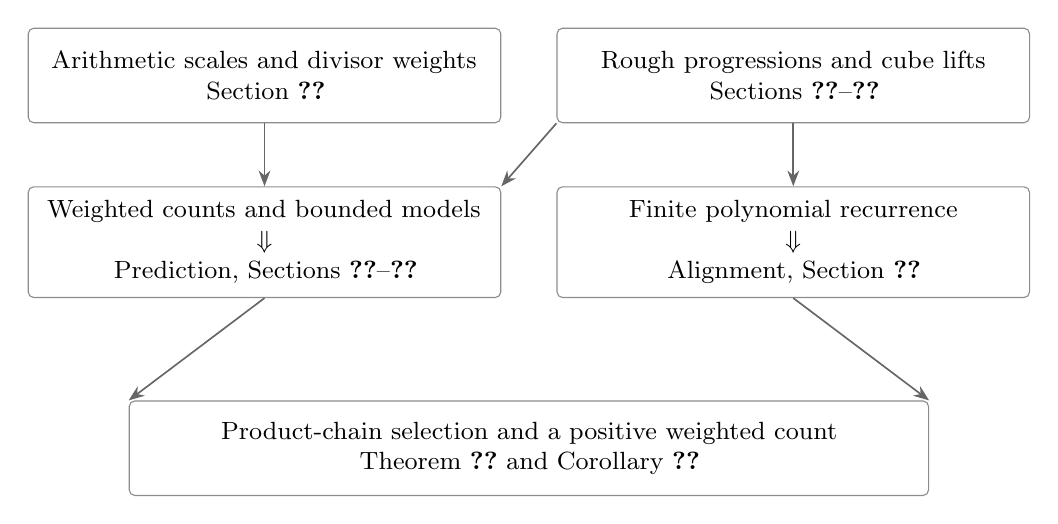
\begin{tikzpicture}[
 node distance=8mm and 7mm,
 box/.style={draw=black!45,rounded corners=2pt,align=center,
 text width=5.65cm,minimum height=12mm,inner sep=5pt,font=\small},
 result/.style={box,text width=9.8cm},
 arr/.style={-{Stealth[length=2mm]},semithick,draw=black!60}]
 \node[box] (weights) {Arithmetic scales and divisor weights\\
   Section~\ref{sec:arithmetic}};
 \node[box,right=of weights] (geometry) {Rough progressions and cube lifts\\
   Sections~\ref{sec:rough-progressions}--\ref{sec:cube-limits}};
 \node[box,below=of weights] (prediction) {Weighted counts and bounded models\\
   $\Downarrow$\\Prediction, Sections~\ref{sec:correlation}--\ref{sec:prediction}};
 \node[box,below=of geometry] (alignment) {Finite polynomial recurrence\\
   $\Downarrow$\\Alignment, Section~\ref{sec:alignment}};
 \path (prediction.south) -- (alignment.south)
   node[midway,below=13mm,result] (deduction)
   {Product-chain selection and a positive weighted count\\
    Theorem~\ref{thm:main} and Corollary~\ref{cor:distinct-expressions}};
 \draw[arr] (weights) -- (prediction);
 \draw[arr] (geometry) -- (alignment);
 \draw[arr] (geometry.south west) -- (prediction.north east);
 \draw[arr] (prediction.south) -- (deduction.north west);
 \draw[arr] (alignment.south) -- (deduction.north east);
\end{tikzpicture}
\caption{The main analytic routes meet in the combinatorial deduction.
The diagonal arrow records the shared missing-corner reconstruction
from Lemma~\ref{lem:cube-corner}.
Alignment fixes a positive mass before Prediction fixes model complexity;
this order permits the counting error to be made small enough.}
\label{fig:proof-map}
\end{figure}

\section{Two principles and the combinatorial deduction}
\label{sec:framework}

We first state the two analytic principles in the precise forms used to
prove Theorem~\ref{thm:main}. This also fixes the order of all parameters.
The proof of the Prediction Principle occupies
Sections~\ref{sec:arithmetic}--\ref{sec:prediction}, with the independent
missing-corner Lemma~\ref{lem:cube-corner} proved in
Section~\ref{sec:cube-limits}.
Sections~\ref{sec:rough-progressions} and~\ref{sec:cube-limits} develop the
nilsequence tools for the Alignment Principle, proved in
Section~\ref{sec:alignment}.

\subsection{Ordered blocks and admissible scales}

For nonempty subsets $A,B\subseteq[n]$,
$A<B$ means $\max A<\min B$; we write $A<i$ for $A<\{i\}$.
For a list of multiplicative quantities $u_1,\ldots,u_n$, put
$u_A=\prod_{j\in A}u_j$. In particular this convention applies to
$t_A,h_A,b_A$, and $x_A$. Empty products, when they occur, equal one.

A \emph{block} is a set $B=T\cup\{i\}$ with $\varnothing\ne T<i$.
We call $i$ its \emph{pivot} and $T$ its \emph{tail}. For such a block let
\begin{equation}\label{eq:adding-blocks}
 \mathcal E_B=
 \bigl\{P\cup\{j\}:\varnothing\ne P<T<j<i\bigr\}.
\end{equation}
These are the blocks whose values will be added at the anchor $B$.
A \emph{chain of length $m$} is a list
$B_d=T_d\cup\{i_d\}$, $d\in[m]$, satisfying
\begin{equation}\label{eq:block-chain}
 \varnothing\ne T_1<T_2<\cdots<T_m<i_1<\cdots<i_m.
\end{equation}
All blocks in a chain are disjoint. Moreover, if $k<d$, then
$B_k\in\mathcal E_{B_d}$. This last property is why we use this particular
ordering of tails and pivots.

All asymptotic parameters below are indexed by positive integers
$w\to\infty$, and
\[
 W=W(w)=\prod_{p\le w}p,
\]
where the product is over primes. An integer is \emph{$w$-smooth} if all
its prime factors are at most $w$. We say that a positive quantity $A$
\emph{dominates powers} of a quantity $B\ge2$ if
$A/B^C\to\infty$ for every fixed $C>0$. Every finite index set,
complexity bound and tolerance is held fixed in this convention unless
additional uniformity is stated. Sampling an interval always means
sampling its integer points.

Fix once and for all a nonprincipal ultrafilter $\mathcal U$ on the
positive integers $w$, and write $\lim_{\mathcal U}$ for its limit.
Every bounded real sequence has such a limit, and it agrees with the
ordinary limit when that exists. Every set belonging to $\mathcal U$
meets every sufficiently late range of $w$. These are the limit and
extraction properties used below.

\begin{definition}[Admissible parameters]\label{def:admissible}
For a fixed $n$, an admissible family consists of positive integers
$M,h_1,\ldots,h_n,H_1,\ldots,H_n$, positive powers of two
$X_1,\ldots,X_n$, and independent random variables $t_1,\ldots,t_n$,
all depending on $w$, with the following properties.
\begin{enumerate}
\item $M$ and each $h_i$ are $w$-smooth multiples of $W^w$.
For every block $B$, and also for every singleton $\{i\}$,
$h_B\le M$. For every $A\in\mathcal E_B$, the ratio $h_A/h_B$
is an integer multiple of $W^w$.
\item Each $H_i$ is a multiple of $M$ and dominates powers of
$2+M+\prod_{\ell<i}X_\ell$. The quantity $\log X_i$ dominates powers
of $H_i$.
\item The law of $t_i$ is the harmonic $W$-unit probability measure
\begin{equation}\label{eq:harmonic-law}
 \mu_i(y)=\frac{\1_{X_i\le y<X_i^2}\1_{(y,W)=1}}{Z_i y},
 \qquad
 Z_i=\sum_{\substack{X_i\le y<X_i^2\\(y,W)=1}}\frac1y.
\end{equation}
\end{enumerate}
\end{definition}

Fixed positive rational factors have only finitely many denominator
primes and fixed denominator valuations. Consequently they can be
absorbed by $W^w$ for all sufficiently large $w$. In particular, every
color argument used below is eventually a positive integer. For a chain
and fixed positive rational $a_1,\ldots,a_m$, the ratios
$h_{B_k}a_k/(h_{B_d}a_d)$, $k<d$, are eventually positive integers:
the pair belongs to \eqref{eq:adding-blocks}. These facts allow us to
use rational scale lists without ever evaluating the coloring on a
noninteger.

\subsection{Piecewise nilsequence models}

A \emph{nilsequence of step at most $s$} is a sequence
\begin{equation}\label{eq:nilsequence-definition}
 k\longmapsto F(g^k x),\qquad k\in\Z,
\end{equation}
where $G$ is a connected simply connected nilpotent Lie group of step
at most $s$, $\Gamma\subset G$ is a lattice, $x\in G/\Gamma$, $g\in G$,
and $F$ is a Lipschitz function on $G/\Gamma$.
Throughout this paper a family has \emph{bounded complexity} if its
nilmanifolds belong to a fixed finite list and its observables have
uniformly bounded supremum and Lipschitz norms for fixed smooth metrics.
No bound is imposed on the translating elements $g$ or the points $x$.
Constants are included. Products and Lipschitz combinations of any
fixed finite number of such families remain bounded-complexity
nilsequences of the same maximal step, by taking product nilmanifolds.

\begin{definition}[Piecewise models]\label{def:piecewise-model}
Fix finite sets $\mathcal A\subset\Q_{>0}$ and $[r]$, and an admissible
family. A system of step-at-most-$s$ models consists of functions
$S_{B,a,c}:\Z\to[0,1]$, one for each block $B$, $a\in\mathcal A$,
and $c\in[r]$. If $i=\max B$, then on each interval
$[kH_i,(k+1)H_i)$ and each residue class modulo $M$, the function is a
nilsequence in the progression index. The complexity is bounded
uniformly over $w$, all pieces, and all model indices. The representing
observables may be, and are, chosen $[0,1]$-valued on their entire
nilmanifolds.
\end{definition}

The sequence and its nilmanifold may change from piece to piece within
the fixed finite list. This freedom is necessary in the inverse-theorem
argument. Real parts followed by clipping to $[0,1]$ justify the final
sentence of Definition~\ref{def:piecewise-model} without increasing the
nilpotence step.

For a block $B=T\cup\{i\}$ define its divisor weight on all of $\Z$ by
\begin{equation}\label{eq:divisor-weight}
 \nu_B(y)=\E_{\sigma=t_T}\sigma\1_{\sigma\mid y}.
\end{equation}
The expectation uses the raw laws of the tail variables only.
For a fixed tail product $\sigma$, we have $(\sigma,W)=1$, so
the conditional mass of $\sigma t_i$ at $y$ is
\[
 \frac{\sigma\1_{\sigma\mid y}\1_{(y,W)=1}}{Z_i y}
 \quad\text{on }[\sigma X_i,\sigma X_i^2).
\]
Thus $\nu_B$ averages the divisibility factor inserted by multiplication
by the tail. Corollary~\ref{cor:product-law} controls the change of
endpoints back to $[X_i,X_i^2)$ and shows that the sum of the absolute
differences between the masses of $\operatorname{Law}(t_B)$ and
$\nu_B\mu_i$ tends to zero.
Whenever several copies of a weight are expanded, they receive
independent divisor samples. In particular, two occurrences of
$\nu_B$ do not share a sample unless this is expressly stated.

\subsection{Prediction and alignment}

We use finite lists $\mathcal B\subset\Q_{>0}^n$ and
$\mathcal A\subset\Q_{>0}$ satisfying
\begin{equation}\label{eq:scale-list-closure}
 b_B\in\mathcal A\quad\text{for all }b\in\mathcal B
 \text{ and all blocks }B.
\end{equation}
The coloring is a map $\chi:\N\to[r]$.

\begin{principle}[Prediction]\label{pr:prediction}
For every $m\ge2$ there is an integer $s=s(m)$ with the following
property. Given $n,r,\chi$, finite lists satisfying
\eqref{eq:scale-list-closure}, and tolerances
$0<\tau<1/4$, $\eta>0$, there are admissible parameters and
step-at-most-$s$ models such that the following conclusions hold along
the fixed ultrafilter $\mathcal U$ in $w$.
\begin{enumerate}
\item For each $B,a,c$,
\begin{equation}\label{eq:prediction-calibration}
 \lim_{\mathcal U}\PP\bigl(
 \chi(h_Bat_B)=c,\ S_{B,a,c}(t_B)\le2\tau\bigr)
 \le3\tau+\eta.
\end{equation}
\item Fix a chain $B_1,\ldots,B_m$, $b\in\mathcal B$ and a color
$c\in[r]$. Put
\[
 c_d=h_{B_d}b_{B_d},\qquad
 f_d(y)=\1_{\chi(c_dy)=c},\qquad
 \nu_d=\nu_{B_d},\qquad S_d=S_{B_d,b_{B_d},c}.
\]
Here $f_d$ is defined on positive integers and may be extended by zero
elsewhere. For $\varnothing\ne J\subseteq[m]$ write $d(J)=\max J$ and
\begin{align}
 L_J(z)&=\sum_{k\in J}\frac{c_k}{c_{d(J)}}z_k,
 \label{eq:sum-forms}\\
 U(z)&=\prod_{\varnothing\ne J\subseteq[m]}
 \1_{\chi(\prod_{k\in J}c_kz_k)=c}.
 \label{eq:product-mask}
\end{align}
Then the nonnegative weighted count
\begin{equation}\label{eq:weighted-count}
 \mathcal I_{b,c,\mathbf B}=
 \E_{z\sim\bigotimes_{d=1}^m\mu_{i_d}}
 U(z)\prod_{d=1}^m\nu_d(z_d)
 \prod_{\substack{J\subseteq[m]\\|J|\ge2}}
 (f_{d(J)}\nu_{d(J)})(L_J(z))
\end{equation}
satisfies, for $z(t)_d=t_{B_d}$,
\begin{equation}\label{eq:prediction-counting}
 \lim_{\mathcal U}
 \abs*{\mathcal I_{b,c,\mathbf B}
 -\E_t U(z(t))
 \prod_{\substack{J\subseteq[m]\\|J|\ge2}}
 S_{d(J)}(L_J(z(t)))}\le\eta.
\end{equation}
\end{enumerate}
\end{principle}

The step bound depends only on the requested chain length $m$.
The complexity bound may depend on all the fixed data and tolerances.
The extra weights on the sum forms in \eqref{eq:weighted-count} are
deliberate: they put the function at each sum under the same majorant
as the function at its last summand. Positivity of this weighted count
still gives an actual monochromatic configuration.

\begin{principle}[Alignment]\label{pr:alignment}
For every $n,r,s$ there are finite lists $\mathcal B,\mathcal A$
satisfying \eqref{eq:scale-list-closure} and a constant $\delta>0$,
depending only on $n,r,s$, such that the following holds.
For any admissible family, any system of step-at-most-$s$ models, and
any fixed $\tau>0$, define $\mathsf A_w$ to be the event that some
$b\in\mathcal B$ satisfies, simultaneously for every block $B$, color
$c\in[r]$, and subset $D\subseteq\mathcal E_B$,
\begin{equation}\label{eq:alignment-implication}
 \begin{split}
 S_{B,b_B,c}(t_B)>2\tau\quad\Longrightarrow\quad
 S_{B,b_B,c}\left(
 t_B+\sum_{A\in D}\frac{h_Ab_A}{h_Bb_B}t_A\right)>\tau.
 \end{split}
\end{equation}
Then
\begin{equation}\label{eq:alignment-probability}
 \liminf_{w\to\infty}\PP(\mathsf A_w)\ge\delta.
\end{equation}
In particular, $\delta$ is independent of $\tau$ and of the model
complexity bound.
\end{principle}

There is no assertion of a convergence rate uniform over all
complexities in \eqref{eq:alignment-probability}. Its positive lower
bound is uniform. This distinction allows us to choose the small
calibration tolerance before constructing the models.

\subsection{A finite combinatorial selection}

We use the finite sums theorem in its following finite form: for every
$m,r$ there is $F=F(m,r)$ such that every coloring of $[F]$ with $r$
colors contains positive integers $u_1,\ldots,u_m$ whose nonempty subset
sums all lie in $[F]$ and have one color. This is the finite sums theorem
of Folkman--Rado--Sanders \cite[Theorem~2 and Corollary~1.1]{Sanders};
it also follows from Hindman's finite sums theorem and compactness
\cite{Hindman,HindmanStrauss}. Indeed, if the finite form failed,
the finitely branching tree of bad finite colorings, ordered by restriction,
would have an infinite branch. Its limiting coloring of $\N$ would
contradict the finite sums theorem. We require no distinctness of
the auxiliary $u_d$ here.

The following selection uses the Ramsey-by-cardinality and finite-sums
argument of \cite[Section~5, Steps~II--IV]{Alweiss}; the ordered tails
and pivots are chosen to match the additive shifts in
\eqref{eq:adding-blocks}.

\begin{lemma}[Selection of a product chain]\label{lem:chain-selection}
For every $m,r$ there is $n=n(m,r)$ such that, for every coloring
$\chi:\N\to[r]$ and every list $x_1,\ldots,x_n\in\N$, a chain
$B_1,\ldots,B_m$ has all nonempty products of
$x_{B_1},\ldots,x_{B_m}$ in a single color class.
\end{lemma}

\begin{proof}
Choose $F$ as above and put $n_0=2F$. Repeated finite Ramsey gives
an $n$ such that every coloring of the nonempty index subsets of
$[n]$ has an $n_0$-element subset on which the color depends only on
cardinality, when the number of colors is $r$. More precisely, apply
the finite Ramsey theorem successively to the subset sizes
$1,\ldots,n_0$, choosing the successive ambient bounds backward.
Apply this to the coloring $A\mapsto\chi(x_A)$, and call the
resulting cardinality color $\kappa(q)$, $1\le q\le n_0$.

Color $a\in[F]$ by $\kappa(2a)$. Choose $u_1,\ldots,u_m$ by the
finite sums theorem and put $q_d=2u_d$. Then $q_d\ge2$,
$\sum_dq_d\le n_0$, and all nonempty subset sums of the $q_d$ have
the same $\kappa$-color. In the homogeneous ordered index set,
choose successive groups of $q_1-1,\ldots,q_m-1$ indices for
$T_1,\ldots,T_m$, followed by $m$ indices for the pivots
$i_1<\cdots<i_m$. This uses $\sum_dq_d$ indices and satisfies
\eqref{eq:block-chain}. A product of the corresponding block
products is $x_{\bigcup_{d\in J}B_d}$, whose index-set size is
$\sum_{d\in J}q_d$. All these sizes have the chosen color.
\end{proof}

\subsection{Deduction of the main theorem}

\begin{proof}[Proof of Theorem~\ref{thm:main}, assuming the two principles]
The case $m=1$ follows by choosing any integer $a_1>R$.
For $m\ge2$, fix $s=s(m)$ from
Principle~\ref{pr:prediction} and $n=n(m,r)$ from
Lemma~\ref{lem:chain-selection}. Apply Principle~\ref{pr:alignment}
to fix $\mathcal B,\mathcal A$ and $\delta>0$.
Let $C$ be the number of triples $(B,a,c)$ indexing calibration
events, and let $K$ be the number of triples consisting of a scale
vector, a chain of length $m$, and a color. These are fixed finite
numbers depending on data already chosen.

Choose $0<\tau<1/4$ and then $\eta>0$ so that
\begin{equation}\label{eq:outer-tolerances}
 3C\tau<\frac\delta4,\qquad
 C\eta<\frac\delta4,\qquad
 K\eta<\frac{\delta\tau^{2^m}}4.
\end{equation}
Now apply Principle~\ref{pr:prediction}. Define $\mathsf G_w$ to
be the event that none of its calibration failures occurs. The
union bound and \eqref{eq:prediction-calibration} give
\[
 \lim_{\mathcal U}\PP(\mathsf G_w^c)
 \le C(3\tau+\eta)<\frac\delta2.
\]
Since an ordinary lower limit bounds every ultrafilter limit,
\eqref{eq:alignment-probability} yields
\begin{equation}\label{eq:good-alignment-mass}
 \lim_{\mathcal U}\PP(\mathsf A_w\cap\mathsf G_w)
 \ge\frac\delta2.
\end{equation}

On this intersection choose a witnessing $b\in\mathcal B$ and
apply Lemma~\ref{lem:chain-selection} to
$x_i=h_ib_it_i$, which are positive integers for all sufficiently
large $w$. It supplies a chain and a color $c$ for which
$U(z(t))=1$. In particular, the singleton product masks say
$\chi(h_{B_d}b_{B_d}t_{B_d})=c$ for every $d$. Because
$\mathsf G_w$ holds, all centers $S_d(t_{B_d})$ exceed $2\tau$.

For a nonsingleton $J\subseteq[m]$, let $d=\max J$. Each
$B_k$, $k\in J\setminus\{d\}$, belongs to $\mathcal E_{B_d}$.
The corresponding instance of \eqref{eq:alignment-implication}
therefore gives
\[
 S_d\bigl(L_J(z(t))\bigr)>\tau.
\]
There are $q=2^m-m-1$ such factors. Thus at least one of the $K$
nonnegative model integrands in \eqref{eq:prediction-counting}
is greater than $\tau^q\ge\tau^{2^m}$ on
$\mathsf A_w\cap\mathsf G_w$. Summing expectations and using
\eqref{eq:good-alignment-mass} shows that their sum has ultrafilter
limit at least $\delta\tau^{2^m}/2$. It follows from
\eqref{eq:prediction-counting} and \eqref{eq:outer-tolerances} that
\begin{equation}\label{eq:positive-total-count}
 \lim_{\mathcal U}
 \sum_{b,c,\mathbf B}\mathcal I_{b,c,\mathbf B}>0.
\end{equation}
In particular, the finite sum is bounded below by a positive number
on a set belonging to $\mathcal U$. We did not need a fixed
choice of witnessing chain across different samples or values of $w$.

For some sufficiently large $w$, one weighted count is positive.
Since it is a finite nonnegative average, there is an actual tuple
$z$ in its support for which every factor is positive. Put
$a_d=c_dz_d$. The product mask gives every nonempty product of
the $a_d$ in color $c$, including their singleton values.
For every nonsingleton $J$, positivity of its color factor gives
\[
 \chi\left(c_{d(J)}L_J(z)\right)
 =\chi\left(\sum_{k\in J}a_k\right)=c.
\]
The extra divisor factors cannot create a false positive; they only
restrict which tuples can contribute to the count.

It remains to obtain the prescribed separation. The finite rational scale lists
give a constant $C_0$ such that $c_d\le C_0M$ for all these counts,
and $c_d\ge1$ once it is a positive integer. If $d<e$, then
\[
 a_d<C_0M X_{i_d}^2,\qquad a_e\ge X_{i_e}.
\]
For $e\ge2$, put $V_e=2+M+\prod_{j<i_e}X_j$.
There is a constant $C_1$, depending only on the fixed finite data,
such that every support tuple satisfies
\[
 \sum_{d<e}a_d+\prod_{d<e}a_d\le C_1 V_e^{3m}.
\]
Indeed each preceding $a_d$ is at most $C_0V_e^3$, and there are
at most $m-1$ such terms. Admissibility makes $X_{i_e}$ dominate
every fixed power of $V_e$. Therefore, for the prescribed $R,D$,
all support tuples at sufficiently large $w$ satisfy
\eqref{eq:separated-elements}; the first element exceeds $R$ since
$a_1\ge X_{i_1}\to\infty$. The positive-count set in
\eqref{eq:positive-total-count} belongs to the nonprincipal
ultrafilter and hence meets every sufficiently late range of $w$.
Choose $w$ in that intersection. This proves both monochromaticity
and separation, and completes Theorem~\ref{thm:main}.
\end{proof}

\begin{proof}[Proof of Corollary~\ref{cor:distinct-expressions}]
Apply Theorem~\ref{thm:main} with $R=2$ and $D=1$.
Every $a_j$ exceeds the sum and the product of all its predecessors,
and every element is at least two. If two subset sums were equal,
cancel their common terms. The greatest remaining index on either
side would exceed the sum on the other side, a contradiction.
For products, cancel common factors and compare the greatest
remaining factor with the product of all preceding factors.
An empty side after cancellation equals one, which is also smaller
than every remaining factor. Thus both subset maps are injective.

To compare a subset sum with a subset product, first compare their
greatest indices. If these differ, the expression with the larger
index exceeds the other expression. If both have greatest index $j$,
the sum lies in $[a_j,2a_j)$, whereas a nonsingleton product is at
least $2a_j$. A singleton product equals $a_j$, which equals a sum
with greatest index $j$ only for the singleton sum. Hence the
intersection is exactly $A$, giving the stated cardinalities.
\end{proof}

\begin{corollary}[Finite interval form with prescribed divisibility]
\label{cor:finite-interval}
Fix integers $r,m,q\ge1$ and real numbers $R\ge2$, $D\ge1$.
There exists $N$ such that every $r$-coloring of $[N]$ admits
$A=\{a_1<\cdots<a_m\}\subset q\N$ with
$\FS(A)\cup\FP(A)\subseteq[N]$ monochromatic and
\[
 a_1>R,\qquad
 a_d>R\left(\sum_{k<d}a_k+\prod_{k<d}a_k\right)^D
 \quad(2\le d\le m).
\]
The subset sums and products have the distinctness properties of
Corollary~\ref{cor:distinct-expressions}.
\end{corollary}

\begin{proof}
First color all of $\N$, refining the given color by the residue
modulo $q$. Apply Theorem~\ref{thm:main} to this finite coloring
with $\max(m,2)$ elements. Their common residue $v$ also equals
the residue of the sum of the first two elements, so $v=2v$
modulo $q$ and $v=0$. Retain the first $m$ elements. The
separation and monochromaticity persist, and the preceding proof
gives the distinctness assertions.

If no $N$ worked, the finite colorings avoiding such a configuration
would form a finitely branching tree, closed under restriction and
with a node at every depth. An infinite branch would color $\N$
without the configuration just proved to exist. Indeed each finite
configuration and all its sums and products lie in some initial
interval. This contradiction proves the finite interval assertion.
\end{proof}

This compactness argument gives a finite bound, but the proof does
not supply a numerical estimate for $N$.

\section{Arithmetic scales and divisor weights}\label{sec:arithmetic}

Prediction compares a count sampled at the pivots with a count sampled
at the block products.  For a block \(B=T\cup\{i\}\), conditioning on
\(\sigma=t_T\) changes the harmonic density of \(t_i\) to
\(\sigma\1_{\sigma\mid y}/(Z_i y)\) on
\([\sigma X_i,\sigma X_i^2)\), with the same \(W\)-unit restriction.
Averaging the divisibility factor gives \(\nu_B\).  We first show that
returning the endpoints to \([X_i,X_i^2)\) has negligible total mass.

We then construct scales and prime parameters for the correlation
argument.  The prime laws have enough harmonic mass to permit prime
insertion, and their residue uniformity makes products of divisor
weights have mean one on the required linear systems.  A separate
coprimality estimate for independent polynomial values will allow
Section~\ref{sec:prediction} to combine cube tests with different
prime-dependent step sizes.

We use \emph{rough} to mean coprime to \(W=\prod_{p\le w}p\), and put
\[
 |a|_{>w}=\prod_{p>w}p^{v_p(a)}\qquad(a\in\Z\setminus\{0\}).
\]
All finite templates in this Section are fixed before the limit
\(w\to\infty\).  A template specifies numbers of variables and rows,
block sizes, and integer polynomials, but no color functions.

\subsection{Harmonic sampling identities}

We give explicit total-mass bounds to distinguish multiplication of
an argument from conditioning on divisibility.  For a signed measure
on \(\Z\), write \(\|\xi\|_1=\sum_{n\in\Z}|\xi(n)|\).
Thus probability total variation is one half of this norm.

\begin{lemma}[Sampling and changes of variables]\label{lem:sampling}
Let \(X\ge2\) be an integer, set
\[
 \vartheta_W=\frac{\phi(W)}W,\quad L_X=\log X,\quad
 Z_X=\sum_{\substack{X\le n<X^2\\(n,W)=1}}\frac1n,\quad
 \mu_X(n)=\frac{\1_{[X,X^2)}(n)\1_{(n,W)=1}}{nZ_X},
\]
and suppose \(L_X>W/X\).  Let \(Y\) have law \(\mu_X\).
\begin{enumerate}
\item For \((k,W)=1\), every residue \(a\pmod k\), and
\(0<A<B\),
\begin{equation}\label{eq:periodic-harmonic}
 \left|\sum_{\substack{A\le n<B\\(n,W)=1\\n\equiv a\ (k)}}\frac1n
  -\frac{\vartheta_W}{k}\log\frac BA\right|
 \le\frac{\phi(W)}A.
\end{equation}
In particular \(|Z_X-\vartheta_WL_X|\le\phi(W)/X\), and
\begin{equation}\label{eq:harmonic-residue-error}
 \left|k\PP(Y\equiv a\pmod k)-1\right|
 \le E_X(k):=\frac{W(k+1)}{X(L_X-W/X)}.
\end{equation}
The total-mass distance of the residue law from uniform measure is
also at most \(E_X(k)\).
\item If \(h\in W\Z\), then
\begin{equation}\label{eq:harmonic-translation}
 \|\operatorname{Law}(Y+h)-\mu_X\|_1
 \le \min\left(2,\frac{2|h|}{X(L_X-W/X)}\right).
\end{equation}
\item If \(1\le k\le X\) and \((k,W)=1\), let
\(\eta_k(n)=k\1_{k\mid n}\mu_X(n)\), an unnormalized positive
measure.  Then
\begin{equation}\label{eq:harmonic-dilation}
 \|\operatorname{Law}(kY)-\eta_k\|_1
 \le\frac{2\log k+(Wk/X)(1+1/X)}{L_X-W/X},
\end{equation}
and \(|\eta_k(\Z)-1|\le E_X(k)\).
\end{enumerate}
For the asymptotic conclusions, let \(K,H,V\ge1\) be auxiliary
quantities depending on \(w\).  Each residue and translation error is
\(o(V^{-C})\), for every fixed \(C\), uniformly for
\(k\le K\) and \(|h|\le H\), if \(X\) dominates every fixed
power of \(2+W+K+H+V\).  The dilation error has the same conclusion
if \(\log X\) dominates every fixed power of \(2+W+K+V\).
These conclusions still hold in expectations of functions bounded
by any fixed power of \(V\).
\end{lemma}

\begin{proof}
The indicator in \eqref{eq:periodic-harmonic} is periodic modulo
\(Wk\) and occupies exactly \(\phi(W)\) residue classes.  On any
interval, its counting function differs from
\(\vartheta_W/k\) times length by at most \(\phi(W)\): apply
the discrepancy bound of one to each occupied class.  Partial
summation against \(1/t\) gives \eqref{eq:periodic-harmonic}.
Apply it with \(k=1\) to obtain the bound on \(Z_X\).
For a general class the error in its unnormalized mass is at most
\(\phi(W)/X\); subtracting \(Z_X/k\) and using
\(Z_X\ge\vartheta_W(L_X-W/X)\) proves
\eqref{eq:harmonic-residue-error}.  Sum the absolute class errors
to obtain the total-mass assertion.

For translation put \(H=|h|\).  Translation invariance of the norm
reduces to \(h=H\ge0\).  On the overlap of the supports,
\(1/(n-H)\ge1/n\), and \(W\mid H\) preserves the unit
condition.  The negative part of
\(\operatorname{Law}(Y+H)-\mu_X\) is therefore precisely the
original mass on \([X,\min(X+H,X^2))\).  Both measures have
mass one, so the norm is twice that mass.  If
\(H\le X^2-X\), the interval \([X,X+H)\) has exactly
\(\vartheta_WH\) units modulo \(W\), since its integer length
is a multiple of \(W\); its harmonic mass is at most
\(\vartheta_WH/X\).  If \(H>X^2-X\), the norm is at most two,
and the second bound in \eqref{eq:harmonic-translation} is already
at least two.  This proves the translation estimate.

For dilation, at a multiple \(n\) of \(k\) the pushed-forward
mass is \(k/(nZ_X)\), supported on \([kX,kX^2)\) and on
\((n,W)=1\).  Thus it agrees exactly with \(\eta_k\) on the
overlap.  Changing variables \(n=ku\) in the two boundary pieces,
and using \(k\le X\), gives the exact formula
\begin{align*}
 \|\operatorname{Law}(kY)-\eta_k\|_1
 =\frac1{Z_X}\bigg(
  \sum_{\substack{X/k\le u<X\\(u,W)=1}}\frac1u
  +\sum_{\substack{X^2/k\le u<X^2\\(u,W)=1}}\frac1u
 \bigg).
\end{align*}
Each main term in \eqref{eq:periodic-harmonic} is
\(\vartheta_W\log k\), and the two errors are at most
\(\phi(W)k/X\) and \(\phi(W)k/X^2\), respectively.
Dividing by the lower bound for \(Z_X\) proves
\eqref{eq:harmonic-dilation}.  Its mass assertion follows from
\eqref{eq:harmonic-residue-error} with \(a=0\).
Finally, integration against a function of supremum norm \(B\)
costs at most \(B\) times the total-mass error.  The stated growth
conditions absorb every fixed choice of \(B=V^{O(1)}\).
\end{proof}

For later use, uniform sampling on an integer interval of length
\(T\) has residue law modulo \(k\) at total-mass distance at most
\(2k/T\) from uniform measure.  Each residue occurs either
\(\lfloor T/k\rfloor\) or \(\lceil T/k\rceil\) times, up to
the harmless endpoint convention.  The same bound is uniform in
the interval's location.  Translating the interval by an integer
\(u\) changes its probability law in total-mass norm by at most
\(2\min(1,|u|/T)\).  Product laws incur the sum of the coordinate
errors, by telescoping their tensor products.  These facts and
Lemma~\ref{lem:sampling} apply conditionally when the interval
endpoints, dilations, or translations have been fixed by outside
variables and the displayed bounds hold uniformly in those variables.

\subsection{Recovering the product sampling law}

The next Corollary identifies the center weights in
\eqref{eq:weighted-count} with the actual block-product sampling.
Once the shifted factors have bounded models, this identity will remove
the remaining weights from the count.

\begin{corollary}[Product law]\label{cor:product-law}
Let \(B=T\cup\{i\}\) be a block, and let \(t_j\) be the
independent harmonic samples at its raw cutoffs.  Let \(V=V(w)\ge1\)
be an auxiliary scale, and put
\(K_T=\prod_{j\in T}X_j^2\).  If \(\log X_i\) dominates
every fixed power of \(2+W+K_T+V\), then
\begin{equation}\label{eq:block-product-law}
 \left\|\operatorname{Law}(t_B)-
                  \nu_B\mu_i\right\|_1=o(V^{-C})
 \qquad\text{for every fixed }C>0.
\end{equation}
For any fixed family of disjoint blocks the corresponding joint
law differs in the same sense from the product of their weighted
pivot measures, when these hypotheses hold at each pivot.
\end{corollary}

\begin{proof}
Condition on \(\sigma=t_T\).  It is coprime to \(W\),
independent of \(t_i\), and bounded by \(K_T\).  Apply
\eqref{eq:harmonic-dilation} with \(k=\sigma\), uniformly in
this range, and average.  The comparison measure is exactly
\[
 \mu_i(y)\E_{\sigma}\sigma\1_{\sigma\mid y}
     =\mu_i(y)\nu_B(y),
\]
proving \eqref{eq:block-product-law}.  In particular its mass is
\(1+o(V^{-C})\).  Disjoint blocks use disjoint raw variables, so
their original laws are independent.  Telescoping a fixed tensor
product bounds its total-mass error by the sum of the individual
errors times the masses of the other factors, all of which are
\(1+o(1)\).  This proves the joint assertion.
\end{proof}

\subsection{A sequential construction of the master scales}

We now work on a master index set \([N]\). Here \(R_l\) are auxiliary gap
lengths and \(X_j\) are cutoffs for the raw variables.
Section~\ref{sec:prediction} will select the final \(n\) indices and choose
each \(H_i\) from these gap lengths.
The smooth factors \(h_j\) make all required shifts integral.  The prime
pools supply the harmonic mass and residue uniformity described above;
the gap lengths absorb the finitely many polynomial divisibilities
needed by the subsequent changes of variables.  The raw cutoffs are
chosen last in each gap so that the preceding sampling estimates apply.

\begin{lemma}[Master scales]\label{lem:master-scales}
Fix \(N\), a bound on block sizes, a finite set
\(\mathcal A\subset\Q_{>0}\), and a finite list \(\mathcal D\) of
nonzero integer polynomials in finitely many prime-parameter slots.
There are choices of \(h_j,M,X_j,R_l,P_l^-,P_l^+\), for
\(1\le j,l\le N\), with the following properties.
\begin{enumerate}
\item
\(h_j=W^{w2^{N-j}}\), and \(M\) is a power of \(W\), divisible by
\(W^w\), with \(h_j\le M\) for every index and \(h_B\le M\)
for every block under consideration.
Every permitted adding pair satisfies
\(h_A/h_B\in W^w\N\).  For a master chain and
\(c_d=h_{B_d}a_d\), \(a_d\in\mathcal A\), all \(c_d\) are integers
and \(c_u/c_d\in W\N\) when \(u<d\), for sufficiently large \(w\).
\item
There is an integer \(e_0=e_0(w)\) such that, for independent uniform
units in the slots modulo \(W^{e_0}\),
\begin{equation}\label{eq:small-prime-exception}
 \PP\bigl(p^{e_0}\mid D(\boldsymbol u)
       \text{ for some }p\le w,\ D\in\mathcal D\bigr)=o(1).
\end{equation}
Moreover \(W^{e_0+1}c_d\mid M\) for every possible \(c_d\).
\item
Writing
\[
 V_l=2+M+\prod_{j<l}X_j^2,
 \qquad
 Q_l=W^{e_0}\prod_{w<p\le V_l}p,
\]
the pool \(\mathcal P_l\) consists of all primes in a finite union of
consecutive complete dyadic intervals
\([P_l^-,P_l^+)\).  Its law and harmonic mass are
\begin{equation}\label{eq:prime-pool-law}
 H_l^{\rm pr}=\sum_{p\in\mathcal P_l}\frac1p,
 \qquad \lambda_l(p)=\frac1{pH_l^{\rm pr}}.
\end{equation}
Both \(P_l^-\) and \(H_l^{\rm pr}\) dominate every fixed power of
\(V_l\).  The residue law of a sample modulo \(Q_l\) differs from
uniform measure on \((\Z/Q_l\Z)^\times\) by
\(o(V_l^{-C})\) in total variation, for every fixed \(C\).
All slots are sampled independently, including slots in different gaps.
\item
\(R_l\) dominates every fixed power of \(P_l^++V_l\).  It is divisible
by \(M\), by every earlier \(R_j\), and by
\(M|D(\boldsymbol p)|\) for all the nonzero values required for
divisibility in gap \(l\), with these polynomial slots drawn from
that gap's pool.  The integer \(X_l\) is a power of two, and \(\log X_l\)
dominates every fixed power of \(R_l\).
\end{enumerate}
One can include any prescribed finite family of polynomial nonvanishing
conditions in \(\mathcal D\).  Repeated entries and zero values then
have probability \(o(V_l^{-C})\) for every fixed \(C\), whereas the
small-prime exceptions in \eqref{eq:small-prime-exception} have
probability \(o(1)\).
\end{lemma}

\begin{proof}
Set \(e_j=2^{N-j}\).  The strict inequality
\(e_j>\sum_{k>j}e_k\) shows that the sign of
\(\sum_{j\in A}e_j-\sum_{j\in B}e_j\), for distinct subsets, is
determined by the smallest index in their symmetric difference.
For an adding pair that index belongs to \(A\); for two chained
blocks it belongs to the earlier block.  The positive difference is
an integer, so the corresponding ratio of \(h\)-products is divisible
by \(W^w\).  Fixed rational multipliers have bounded valuations and
only finitely many denominator primes.  Consequently they are absorbed
by these powers for all sufficiently large \(w\), leaving at least
one factor of every prime dividing \(W\) in each required ratio of
the \(c_d\)'s.

For completeness, a nonzero polynomial over \(\Q_p\) has a null zero
set in a product of \(p\)-adic unit groups.  In one variable it has
only finitely many roots.  In several variables, expand in a variable
on which it depends and choose a nonzero coefficient polynomial.
By induction, the set on which that coefficient vanishes has measure
zero; off that set, each fiber has finitely many roots.  Fubini's
Theorem proves the assertion.  The decreasing events
\(p^e\mid D\) therefore have probabilities tending to zero as
\(e\to\infty\).  At any fixed \(w\), the list of polynomials and
primes is finite.  Choose a common \(e_0\) making their union
probability at most \(1/w\).  Reduction of uniform units modulo
\(W^{e_0}\) has exactly the required distribution modulo
\(p^{e_0}\).  We can now choose the power \(M\) large enough for
all the finitely many stated smooth divisibilities and bounds.

Proceed in increasing order of \(l\).  At this stage \(Q_l\) is a
fixed integer.  The prime number theorem in each reduced arithmetic
progression modulo \(Q_l\) \cite[Equation~(1.1)]{SelbergAP}, followed by partial summation, says that
the harmonic prime law on \([Y,2Y)\) tends to the uniform law on
its unit classes as \(Y\to\infty\).  Since there are finitely many
classes, choose a dyadic lower endpoint so large that the total
variation error is at most \(V_l^{-w}\) on every subsequent dyadic
interval, and also \(P_l^-\ge wV_l^w\).  Increasing the upper
endpoint gives \(H_l^{\rm pr}\ge wV_l^w\), since the harmonic prime
series diverges.  A mixture of measures having the same error bound
has that error bound.  Thus this finite pool has the asserted
residue distribution, however long the union of intervals is.

Only finitely many polynomial values occur in a finite pool.  Take
their nonzero absolute values, the earlier gap lengths, and \(M\),
form the required least common multiple, and choose a multiple
\(R_l\) at least \(w(P_l^++V_l)^w\).  Finally choose a power of two
\(X_l\) with \(\log X_l\ge wR_l^w\).  There is no upper bound in
any of these choices, and no later requirement changes an earlier
choice.

Here is the elementary zero-value estimate used for the final
assertion.  If independent variables each have maximum atom at most
\(a\), a nonzero polynomial of total degree \(d\) vanishes with
probability at most \(da\).  Expand in its last relevant variable:
outside the zero set of its leading coefficient there are at most
as many roots as its degree in that variable, and induction bounds
the leading-coefficient exception by its degree times \(a\).
For our pool, \(a\le1/(P_l^-H_l^{\rm pr})\); the same estimate for
\(x_i-x_j\) handles repeats.  These bounds are smaller than every
fixed inverse power of \(V_l\). Finally, the residue-law approximation
modulo \(Q_l\), together with the Chinese remainder theorem (CRT),
transfers \eqref{eq:small-prime-exception} to the actual prime slots.
\end{proof}

For a block \(B=T\cup\{i\}\) at these scales, its tail bound
\(K_T\) and \(W\) are at most \(V_i\).  Since \(\log X_i\)
dominates every fixed power of \(V_i\),
Corollary~\ref{cor:product-law} applies with \(V=V_i\).
In particular, the joint law comparison holds for every chain and
hence for bounded expectations of all its block variables.

\begin{remark}[Countably many fixed tests]\label{rem:arithmetic-diagonal}
Later, a fixed test may be raised to any fixed moment or combined
with any fixed number of other tests.  This does not require a
moment order growing inside an estimate.  Enumerate the resulting
integer-polynomial templates and positive integer auxiliary parameters.
At stage \(j\) impose the requirements for the first \(j\) templates.
Each stage has finitely many requirements, so the preceding proof
applies.  Choose increasing thresholds \(w_j\) so that the finitely
many error bounds at that stage, including constants in the estimates
below, are at most \(1/j\) once \(w\ge w_j\).  At a given \(w\)
use stage \(\max\{j:w_j\le w\}\), with the growth exponents also
tending to infinity.  Every fixed finite test family then satisfies
all the conclusions eventually.  This diagonal choice can be made
before the functions to be tested are chosen, because its templates
depend only on their algebraic forms.  All moment limits below mean
first \(w\to\infty\) at a fixed moment order.
\end{remark}

\subsection{Coprimality beyond the CRT cutoff}

The next estimate treats prime factors larger than \(V_l\), as well
as those controlled by the residue distribution of a pool.  The
linear-forms estimate below uses residue uniformity separately.
Coprimality has a different purpose: in a cyclic group, the subgroups
of multiples of two coprime integers together generate the whole group.
Section~\ref{sec:prediction} applies this fact to combine cube tests
with different step sizes.

\begin{lemma}[Rough coprimality]\label{lem:rough-coprimality}
Let \(F\) and \(G\) be fixed nonzero integer polynomials in disjoint
tuples of independent prime variables.  Each variable is sampled with
probability proportional to \(1/p\) in a dyadic interval \([Y,2Y)\).
Let \(L\) be the smallest of these lower endpoints.  For all
sufficiently large \(w,L\),
\begin{align}
 \PP(FG=0)&\ll_{F,G}\frac{\log L}{L},\label{eq:polynomial-zero-bound}\\
 \PP\bigl(FG\ne0,\ \gcd(|F|_{>w},|G|_{>w})>1\bigr)
 &\ll_{F,G}\frac1w+\frac{\log L}{\sqrt L}.
 \label{eq:rough-coprimality-bound}
\end{align}
The constants are independent of the ratios between the dyadic
endpoints.  Consequently two independent tuples from any of the
constructed pools have coprime rough polynomial values with
probability \(1-o(1)\).  The same assertion holds after restricting
each tuple to a prime-only event of probability \(1-o(1)\).
\end{lemma}

\begin{proof}
The prime number theorem gives a maximum atom
\(O(\log Y/Y)\) in the harmonic prime law on \([Y,2Y)\).
The polynomial zero estimate in the proof of
Lemma~\ref{lem:master-scales} proves
\eqref{eq:polynomial-zero-bound}, uniformly in the endpoints.

We shall also use the following consequence of the interval
Brun--Titchmarsh inequality.  If \(p\le\sqrt Y\) is prime, a
harmonically sampled prime in \([Y,2Y)\) belongs to any prescribed
nonzero class modulo \(p\) with probability \(O(1/p)\).
Indeed Theorem~2 of \cite{Yamada}, together with
\(\log(Y/p)\ge\tfrac12\log Y\), bounds the number of primes in a
reduced class in that interval by \(O(Y/(p\log Y))\).
Divide by the prime count \(\gg Y/\log Y\).
Harmonic and uniform sampling on that interval
have densities within a factor of two.  The zero class contains no
prime in \([Y,2Y)\) when \(p\le\sqrt Y\).

Remove variables on which the polynomials do not depend, and argue
by induction on the total number of remaining variables.  A fixed
nonzero constant has no prime factors larger than \(w\) once \(w\)
is large, so it gives the base case.  In each nonconstant polynomial
choose as its main variable one whose interval has largest lower
endpoint in that tuple.  Denote those endpoints by \(Y_F,Y_G\),
and the corresponding nonzero leading-coefficient polynomials by
\(A,B\).  The events \(A=0\) or \(B=0\) cost
\(O_{F,G}(\log L/L)\).  If a common prime divisor of \(F,G\)
also divides \(A\), apply the induction hypothesis to \(A,G\);
if it divides \(B\), apply it to \(F,B\).  The two tuples in each
application remain disjoint, and their total number of variables
strictly decreases.  It remains to consider common primes dividing
neither leading coefficient.

Put \(Y_0=\min(Y_F,Y_G)\).  For \(w<p\le\sqrt{Y_0}\), condition
on all variables except the two main variables.  When the respective
leading coefficient is nonzero modulo \(p\), each polynomial has at
most its fixed degree many roots modulo \(p\).  The preceding
Brun--Titchmarsh consequence bounds the two independent tests by
\(O_{F,G}(p^{-2})\).  Their sum is \(O_{F,G}(1/w)\).

For the remaining primes, expose the entire tuple whose main endpoint
is \(Y_0\), say the \(F\)-tuple.  Every variable in that tuple is
at most \(2Y_0\), so, when \(F\ne0\),
\(1\le |F|\le C_FY_0^{\deg F}\).  It follows that \(F\) has
only \(O_F(1)\) distinct prime divisors exceeding \(\sqrt{Y_0}\).
Test each such prime \(p\) against the independent \(G\)-tuple,
whose main endpoint \(Y=Y_G\) satisfies \(Y\ge Y_0\).  If
\(p\le\sqrt Y\), the cost is \(O_G(1/p)=O_G(Y_0^{-1/2})\),
again excluding the already treated event \(p\mid B\).  If
\(p>\sqrt Y\), each of the boundedly many root classes contains
at most \(Y/p+1\) integers of the interval.  Dividing by
\(\gg Y/\log Y\) gives
\[
 O_G\left(\frac{\log Y}{\sqrt Y}\right)
 =O_G\left(\frac{\log Y_0}{\sqrt{Y_0}}\right).
\]
The last inequality holds for all sufficiently large \(Y_0\), since
\(\log Y/\sqrt Y\) is then decreasing.  Summing over the bounded
number of large prime factors proves the induction and
\eqref{eq:rough-coprimality-bound}.

Conditioning pool samples on their individual dyadic intervals leaves
independent harmonic prime laws.  The established bounds are uniform
over these choices, so averaging proves the pool assertion.
Restricting to events of probabilities \(1-o(1)\) changes any
probability by \(o(1)\).
\end{proof}

The prime pools now have both residue uniformity and rough coprimality.
We turn to the mean-one estimate that permits repeated
Cauchy--Schwarz with divisor weights.

\subsection{The weighted linear-forms estimate}

Recall that for a block \(B=T\cup\{i\}\) and independent tail
product \(\sigma=t_T\), the divisor weight is
\begin{equation}\label{eq:arithmetic-divisor-weight}
 \nu_B(y)=\E_{\sigma}\sigma\1_{\sigma\mid y}.
\end{equation}
In expanding a product of weights, every occurrence of a weight
receives a fresh independent draw, even when its block label repeats.
The next Proposition records precisely the row hypotheses needed
below.  In particular, restrictions on prime parameters are permitted.

The mean-one linear-forms estimate below plays the role of the
pseudorandomness conditions in Green and Tao's transference method
\cite[Definition~3.1 and Section~5]{GreenTaoPrimes}.
We prove the estimate for the present divisor weights and
prime-dependent forms.

\begin{proposition}[Weighted linear forms]\label{prop:linear-forms}
Fix the number \(q\) of rows, the number \(d\) of base variables,
and a bound \(b\) on the number of raw factors in each divisor.
For each \(u\in[q]\), let \(\sigma_u\) be a product of at most
\(b\) independent harmonic \(W\)-unit variables at the master
cutoffs of Lemma~\ref{lem:master-scales}, and write
\(\nu_u(y)=\E\sigma_u\1_{\sigma_u\mid y}\).
All these raw draws are independent across occurrences.  Suppose
\(\sigma_u\le V\) surely, where \(V\ge M\to\infty\).
Let \(\boldsymbol p\) consist of independent prime slots from
finitely many gaps, each having \(V_l\ge V\).  These slots are
independent of all divisor draws.

Let \(\mathcal G\) be a domain depending only on
\(\boldsymbol p\), and let
\(\ell_u(\boldsymbol x;\boldsymbol p)\) be homogeneous linear
rows.  On \(\mathcal G\) their arguments are integers on the
base sampling support.  Assume the following conditions.
\begin{enumerate}
\item Given \(\boldsymbol p\) and any possible divisor draws,
the joint residue law of \(\boldsymbol x\) modulo
\(K=\prod_{u=1}^q\sigma_u\) differs in total variation by at
most \(\epsilon_{\rm base}\) from the uniform law on
\((\Z/K\Z)^d\).  The bound is uniform on \(\mathcal G\).
\item For every \(w<p\le V\), each row is nonzero modulo
\(p\) on \(\mathcal G\).  There is a fixed finite list of
nonzero integer polynomials in the prime slots such that, if all
their values are nonzero modulo \(p\), every pair of rows is
linearly independent over \(\mathbb F_p\).
\end{enumerate}
The CRT law of all prime slots at the primes \(w<p\le V\)
is within total variation \(\epsilon_{\rm CRT}\) of independent
uniform units, with independence also across these primes.
Then, uniformly in every further prime-only event
\(\mathcal E\subseteq\mathcal G\),
\begin{equation}\label{eq:restricted-linear-forms}
 \E_{\boldsymbol p,\boldsymbol x}
   \1_{\mathcal E}(\boldsymbol p)
   \prod_{u=1}^q\nu_u(\ell_u(\boldsymbol x;\boldsymbol p))
 =\PP(\mathcal E)+
 O\left(\frac1w+V^q(\epsilon_{\rm base}+
                              \epsilon_{\rm CRT})\right).
\end{equation}
The error is absolute, so the statement also applies when
\(\PP(\mathcal E)\) tends to zero.
The implied constant depends only on the fixed row and divisor
templates and polynomial tests.  In particular the error is \(o(1)\)
with the scales of Lemma~\ref{lem:master-scales} and base residue
errors smaller than every fixed inverse power of \(V\).

Rows may have rational coefficients if their denominators are units
modulo every possible divisor: interpret their residues by inverting
those denominators.  The integer-value and row hypotheses must still
hold.  Clearing such denominators leaves the congruence calculation
unchanged.  In particular this permits smooth denominators and prime
pool denominators larger than \(V\).
\end{proposition}

\begin{proof}
We first express the normalized divisibility count as a product of local
kernel counts.  Their excess over one is nonnegative; this lets us bound
it without retaining the prime-only event.  We then dominate the divisor
draws by laws with independent prime valuations and sum the local excesses.

\paragraph{Local kernel counts.}
Expand each weight with its independent divisor draw.  Replacing the
base residue law by exact uniform measure modulo \(K\) costs at
most \(2\epsilon_{\rm base}\prod_u\sigma_u
\le2V^q\epsilon_{\rm base}\).  The CRT theorem now factors the
normalized divisibility count as
\[
 \prod_{w<p\le V}\alpha_p,
 \qquad
 \alpha_p=p^{\sum_u a_u}
  \PP_{\boldsymbol x\bmod p^{A}}
       (p^{a_u}\mid\ell_u(\boldsymbol x)\text{ for every }u),
\]
where \(a_u=v_p(\sigma_u)\) and \(A=\max_u a_u\).
Primes with all \(a_u=0\) contribute one.  Homogeneity makes the
divisibility conditions the kernel of a homomorphism into
\(\prod_u\Z/p^{a_u}\Z\).  Its image has size at most
\(p^{\sum a_u}\), so \(\alpha_p\ge1\).  With a single
positive valuation, the corresponding primitive row is surjective
modulo every power of \(p\), giving \(\alpha_p=1\).
In general one primitive row with valuation \(A\) bounds the
kernel probability by \(p^{-A}\).  If the two rows having the
largest valuations \(A\ge B>0\) are independent modulo \(p\),
one of their two-column minors is a unit.  Fixing the other
coordinates, the two selected coordinates are uniformly and
bijectively mapped to the pair of row values modulo \(p^A\).
Their required divisibilities consequently have probability
\(p^{-A-B}\).  Additional rows can only reduce the probability.

We bound the nonnegative excess uniformly, so that an arbitrary
prime-only domain can subsequently be retained.  Let \(\mathcal T_p\)
be the test that at least one of the prescribed polynomial values
vanishes modulo \(p\).  Set \(\beta_p=0\) when fewer than two
valuations are positive; otherwise set
\[
 \beta_p=
 \begin{cases}
 p^{\sum a_u-A-B}-1,&\mathcal T_p\text{ fails},\\
 p^{\sum a_u-A}-1,&\mathcal T_p\text{ holds}.
 \end{cases}
\]
On \(\mathcal G\), the preceding kernel bounds give
\(0\le\alpha_p-1\le\beta_p\).  For every choice of the
parameters and the true, bounded divisor draws,
\begin{equation}\label{eq:local-excess-domination}
 0\le\1_{\mathcal E}
       \left(\prod_p\alpha_p-1\right)
 \le\prod_{w<p\le V}(1+\beta_p)-1
 \le\prod_u\sigma_u\le V^q.
\end{equation}
In particular, we can first replace the prime residues by independent
CRT-uniform units at cost at most \(2V^q\epsilon_{\rm CRT}\).
This replacement is made while all divisor draws are still bounded.

\paragraph{Independent comparison laws.}
We next compare those draws with laws whose prime valuations are
independent.  For a raw factor at cutoff \(X_j\), put
\(\epsilon_j=1/\log X_j\) and define
\[
 \widetilde\mu_j(n)
  =\frac{\1_{(n,W)=1}n^{-1-\epsilon_j}}{
    \zeta(1+\epsilon_j)\prod_{p\le w}(1-p^{-1-\epsilon_j})}
 \qquad(n\ge1).
\]
Its denominator is \((1+o(1))\vartheta_W\log X_j\).
Indeed \(\epsilon\zeta(1+\epsilon)\to1\), and
\[
 0\le\log\prod_{p\le w}
        \frac{1-p^{-1-\epsilon}}{1-p^{-1}}
 \le\epsilon\sum_{p\le w}\frac{\log p}{p-1}
 \le\epsilon\log W=o(1).
\]
Lemma~\ref{lem:sampling} gives the same asymptotic normalization
for the original harmonic law on \([X_j,X_j^2)\), and
\(n^{\epsilon_j}\le e^2\) on that interval.  Hence
\(\mu_j(n)\le C_0\widetilde\mu_j(n)\) pointwise, with an
absolute constant \(C_0\) for sufficiently large \(w\).
For at most \(bq\) independent raw draws this incurs one overall
constant \(C_0^{bq}\), rather than a separate constant for each
prime.

The Euler product defining \(\widetilde\mu_j\) shows that its
valuations at different primes are independent, with
\[
 \widetilde\PP(v_p(n)=a)
    =(1-p^{-1-\epsilon_j})p^{-a(1+\epsilon_j)}
    \le p^{-a}.
\]
Thus a product of at most \(b\) raw factors has valuation mass
at \(a\) at most \((a+1)^b p^{-a}\).  This bound is uniform
in the individual cutoffs.  Divisors remain independent of each
other and of all prime parameters.

\paragraph{Summing the local excesses.}
For sufficiently large \(w\), none of the fixed nonzero test
polynomials is identically zero modulo any prime \(p>w\).
The elementary polynomial root bound on the product grid
\((\mathbb F_p^\times)^k\) gives
\(\PP(\mathcal T_p)=O(1/p)\).  Under the CRT-uniform law the
tests at different primes are independent.  Combining the valuation
bounds with the definition of \(\beta_p\), the contribution when
\(\mathcal T_p\) fails is at most a constant times
\[
 \sum_{A\ge B\ge1}
  (A+1)^{C_1}(B+1)^{C_1}p^{-A-B}
 \ll p^{-2}.
\]
To see this sum explicitly, choose the rows with the two largest
valuations; all other valuations lie between zero and \(B\),
and summing their polynomial factors is bounded by a fixed power
of \(B+1\).  The factors \(p^{-\sum a_u}\) cancel the
normalizing power in \(\beta_p\), leaving \(p^{-A-B}\).
On \(\mathcal T_p\) the same argument, with all lesser
valuations bounded by \(A\), gives
\[
 \sum_{A\ge1}(A+1)^{C_2}p^{-A}\ll p^{-1}.
\]
Its additional \(O(1/p)\) test probability again gives
\(\E\beta_p\ll p^{-2}\).  The two displayed series bounds
follow by factoring out respectively \(p^{-2}\) and \(p^{-1}\)
and bounding the remaining geometrically convergent series using
\(p\ge2\).

We have now obtained independence across primes for every quantity
in the nonnegative right side of
\eqref{eq:local-excess-domination}.  Consequently its expectation,
after the single global divisor-domination constant, is at most
\[
 C_0^{bq}\left\{\prod_{w<p\le V}(1+C_3p^{-2})-1\right\}
 \ll\sum_{p>w}p^{-2}\ll\frac1w.
\]
The original local product has lower bound one on
\(\mathcal E\).  Integrating that lower bound and the estimated
excess, and restoring the two residue-approximation errors, proves
\eqref{eq:restricted-linear-forms}.  Rational denominators which
are units modulo the divisors induce the same homomorphisms after
inversion, so the proof covers the stated rational-row extension.
\end{proof}

Several consequences of Proposition~\ref{prop:linear-forms} will be
used without altering its hypotheses.  A fixed product of factors
\(1+\nu_u\) has main term \(2^q\PP(\mathcal E)\), by expansion
over subsets of rows.  If at least one factor is \(\nu_u-1\),
and the remaining factors are each \(\nu_v\), \(1+\nu_v\),
or \(\nu_v-1\), its average is \(o(1)\), provided every
subsystem in that expansion meets the same row conditions.  This
is cancellation of the constant main terms.  In particular a
prime-only exceptional event of probability \(o(1)\), contained
in a domain of primitive rows, has weighted mass \(o(1)\).
One may also condition on a prime-only event whose probability is
bounded below, dividing \eqref{eq:restricted-linear-forms} by that
probability.

These statements include systems assembled from different gaps.
Use the common divisor bound \(V\); every relevant pool has
\(V_l\ge V\), so projecting its CRT law supplies the required
accuracy.  Independent replicas give independent slots.  For
coefficients involving
\(M(\boldsymbol p)=M|D(\boldsymbol p)|_{>w}\), a prime
\(w<p\le V\) dividing such a coefficient must divide
\(D(\boldsymbol p)\), so the indicated polynomial tests cover
this possible loss of a minor.  Fixed integer contents are
\(w\)-smooth eventually.  Primitivity and separation of each
actual row system still have to be checked; those checks are given
in Sections~\ref{sec:correlation} and \ref{sec:prediction}.

To verify the base-law hypothesis in those applications, every
divisor product \(K\) is at most \(V^q\).  Uniform auxiliary
intervals of lengths dominating all powers of \(V\), and harmonic
pivot variables whose cutoffs dominate all powers of \(W+V\),
are therefore jointly uniform modulo \(K\), with error smaller
than every fixed inverse power of \(V\).  Their conditional
interval locations do not matter.  A short translation changes
such a box by the sum of the displacement-to-side-length ratios;
the translation and dilation bounds above cover harmonic variables.
For example,
\(R_l/(J_0M(\boldsymbol p))\) dominates all powers of the common
tail bound for each fixed \(J_0\), since
\(M(\boldsymbol p)\) has a fixed-power bound in \(P_l^++V_l\).
Taking square roots of these lengths preserves that domination and
gives negligible relative translations.  These observations supply
uniform bounds for the shifted boxes used later, as well as for
unshifted boxes.

\section{Removing multiplicative masks and detecting a shifted error}
\label{sec:correlation}

The purpose of this Section is to turn a correlation containing arbitrary
multiplicative masks into a test of one function on an additive cube.
The number of Cauchy--Schwarz steps will depend only on the number of
blocks in the chain.  This independence from the master index count is
needed when the analytic tolerances are chosen before the Ramsey bound.

Fix a master chain
\[
 B_k=T_k\cup\{i_k\},\qquad
 T_1<\cdots<T_m<l<i_1<\cdots<i_m,
\]
where each tail is nonempty, and fix positive scales
$c_k=h_{B_k}a_k$ from the finite list allowed in
Section~\ref{sec:arithmetic}.  Write $V=V_l$, $R=R_l$, and let
$\mathcal P_l$ be the prime pool in this gap, with law
\[
 \lambda(p)=\frac{1}{pS_l},\qquad
 S_l=\sum_{p\in\mathcal P_l}\frac1p.
\]
In this Section $z_k$ has law $\mu_{i_k}$, independently for different
$k$.  We abbreviate $\nu_k=\nu_{B_k}$, so that $0\le\nu_k\le V$ on
all integers.  For $\emptyset\ne J\subseteq[m]$ put
\[
 a(J)=\max J,\qquad
 L_J(z)=\sum_{k\in J}\frac{c_k}{c_{a(J)}}z_k.
\]
For sufficiently large $w$, all the displayed coefficients are integers,
and every coefficient other than the anchor coefficient is divisible by
$W$.  The scales $c_k$ are positive integers with no prime factor greater
than $w$.  We consider
\begin{equation}
 \mathcal C=
 \E_z\left[
   \prod_{\emptyset\ne U\subseteq[m]}b_U(z_U)
   \prod_{\emptyset\ne J\subseteq[m]}g_J(L_J(z))
 \right],
 \qquad z_U=\prod_{k\in U}z_k,
 \label{eq:correlation-initial}
\end{equation}
where the functions are real, $|b_U|\le1$, and
$|g_J(y)|\le1+\nu_{a(J)}(y)$ for every integer $y$.
Fix $J_*$ with $|J_*|\ge2$, and write $g_*=g_{J_*}$ and
$a_* = a(J_*)$.  Bounded extensions outside the positive integers are
permitted whenever needed.

We will keep one copy of $g_*$ throughout: first remove the product
masks, then eliminate the other linear factors, and finally identify
the sampling law of the surviving cube root.

All estimates below are uniform over these functions.  An $o(1)$ may
depend on the fixed master data and on a fixed positive integer $J_0$,
but not on the functions.  Uniformity also holds over any fixed finite
set of $J_0$'s.  In particular, it does not assert a convergence rate
uniform in a growing master index count.

\subsection{Prime insertion and weighted mask removal}

\begin{lemma}[Prime insertion]\label{lem:prime-insertion}
Let $i>l$ and let $Y$ have law $\mu_i$.  For every fixed $A>0$, uniformly
over functions $F$ with $|F|\le V^A$,
\begin{equation}
 \E_Y F(Y)=\E_{p,Y}F(pY)+o(1).
 \label{eq:prime-average-insertion}
\end{equation}
For a fixed positive integer $k$, coprime to $W$ and bounded by a fixed
power of $P_l^++V$, one also has
\begin{equation}
 \E_Y F(kY)=\E_Y k\1_{k\mid Y}F(Y)+o(1),
 \label{eq:prime-fixed-dilation}
\end{equation}
uniformly in $k$.  The total-mass error before multiplication by $F$ is
smaller than every fixed negative power of $P_l^++V$.
These assertions remain valid with other independent variables as
parameters.
\end{lemma}

\begin{proof}
The dilation assertion is Lemma~\ref{lem:sampling}, applied at a cutoff
whose logarithm dominates all fixed powers of $P_l^++V$.  The weighted
law on the right has the same harmonic density as the law on the left;
only the endpoints $[X_i,X_i^2)$ and $[kX_i,kX_i^2)$ differ.
The logarithmic boundary mass is $O(\log k/\log X_i)$, with the residue
counting error from that Lemma.  The scale separation makes their sum
smaller than any prescribed negative power of $P_l^++V$.

Averaging the multiplier in \eqref{eq:prime-fixed-dilation} gives
\[
 A_l(Y)=\E_p p\1_{p\mid Y}
       =\frac1{S_l}\sum_{p\in\mathcal P_l}\1_{p\mid Y}.
\]
Periodic counting for the moduli $p$ and $pq$, including the $W$-unit
restriction, gives their reciprocal probabilities with uniformly
negligible relative errors.  Therefore
\begin{align*}
 \E A_l&=1+o(V^{-C}),\\
 \E A_l^2
 &=\frac1{S_l^2}
   \left(\sum_p\frac1p+\sum_{p\ne q}\frac1{pq}\right)
   +o(V^{-C})\\
 &=1+\frac1{S_l}-\frac1{S_l^2}\sum_p\frac1{p^2}+o(V^{-C})
\end{align*}
for every fixed $C$.  Thus
$\|A_l-1\|_{L^2(\mu_i)}\le S_l^{-1/2}+o(V^{-C})$.
Cauchy--Schwarz bounds the error in replacing $A_l$ by $1$ by
$V^A(S_l^{-1/2}+o(V^{-C}))=o(1)$, since $S_l$ dominates every fixed
power of $V$.  The estimates are uniform in the parameters of $F$, so
one may integrate over those parameters afterwards.
\end{proof}

A row template will mean a vector $A_R=(A_{R,1},\ldots,A_{R,m})$ whose
nonzero entries are monomials in finitely many formal prime variables.
No prime variable occurs in two different columns of a single row.
For $a(R)=\max\{k:A_{R,k}\ne0\}$, its associated linear form and weight
are
\begin{equation}
 \ell_R(z)=\sum_k\frac{c_k}{c_{a(R)}}A_{R,k}z_k,
 \qquad W_R(y)=1+\nu_{a(R)}(y).
 \label{eq:correlation-row-template}
\end{equation}
Parallelity of templates always means parallelity over the rational
function field in the formal prime variables.  This qualification is
essential: accidental equalities after numerical substitution are
exceptional events, not identities of templates.

Reciprocal dilations preserving a product, followed by
Cauchy--Schwarz to remove its bounded factor, also occur in the proof
of \cite[Proposition~2.4]{GreenSanders} over finite fields.
Here the divisibility weights allow the corresponding substitutions
on integer variables, and we carry out the elimination for the full
family of product masks.

\begin{lemma}[Weighted removal of multiplicative masks]
\label{lem:mask-removal}
Put $q_{\mathrm{mask}}=2^m-1$ and $K_m=q_{\mathrm{mask}}2^{q_{\mathrm{mask}}}$.  Starting from
\eqref{eq:correlation-initial}, one obtains a family $\mathcal R$ of at
most $K_m$ pairwise nonparallel row templates, with one distinguished
row $*$, and functions $f_R$ that may depend on the introduced primes,
such that
\begin{equation}
 |\mathcal C|^{2^{q_{\mathrm{mask}}}}
 \le C_m\left|\E_{\boldsymbol p,z}
                 \prod_{R\in\mathcal R}f_R(\ell_R(z))\right|+o(1).
 \label{eq:mask-removal-output}
\end{equation}
Here $|f_R|\le W_R$, the distinguished function is exactly $f_*=g_*$,
its support is $J_*$, and every prime parameter has the law $\lambda$,
independently before deletion of exceptional tuples.
The row templates, the number of parameters, and $C_m$ depend only on
$m$ and the choice of $J_*$.  They are independent of the scales and
functions.
\end{lemma}

\begin{proof}
Initially the rows are the indicator vectors of the nonempty subsets
$J$ of $[m]$.  They are pairwise nonparallel.  We remove the masks in a
fixed order, maintaining \eqref{eq:correlation-row-template}, the weight
bounds, and a distinguished copy of $g_*$.

\paragraph{A substitution fixing the mask.}
Consider the mask with support $U$.  If the distinguished support has
an index $u\notin U$, use the change $D(p)z$ given by
$z_u\mapsto pz_u$.  Otherwise choose distinct $u,v$ in the distinguished
support, necessarily both in $U$, and use
\begin{equation}
 z_u\mapsto z_u/p,\qquad z_v\mapsto pz_v,
 \qquad \eta_p(z)=p\1_{p\mid z_u}.
 \label{eq:balanced-prime-substitution}
\end{equation}
The first case has $\eta_p=1$.
Lemma~\ref{lem:prime-insertion} justifies the first case directly.
For the second, first insert $p$ in coordinate $v$ and then use
\eqref{eq:prime-fixed-dilation} in coordinate $u$ with the function
read at $z_u/p$.  Thus division by $p$ is used only on the support of
the displayed indicator, and its multiplier is retained.  At this
stage all unweighted functions and all products of row weights are
bounded by a fixed power of $V$; even the intermediate fixed-prime
multipliers are absorbed by the stronger endpoint error in
\eqref{eq:prime-fixed-dilation}.  Both substitutions therefore have
$o(1)$ error.  In either case $z_U$ is unchanged.

Call a row invariant at this step when the coefficient vector of
$\ell_R(D(p)z)$ is a scalar multiple of that of $\ell_R(z)$.
The scalar is $1,p$, or $p^{-1}$.  All divisors in $\nu_{a(R)}$ are
smaller than the pool primes, so multiplication or admissible division
by $p$ preserves their divisibility conditions.  Consequently
\[
 W_R(\ell_R(D(p)z))=W_R(\ell_R(z))
\]
on the support in use.  Put
$\Omega(z)=\prod_{R\text{ invariant}}W_R(\ell_R(z))$.
Divide each invariant function inside the fresh prime average by its
corresponding weight, and call the remaining integrand $H_p$.
Let $\boldsymbol r$ denote all prime slots introduced at earlier steps.
The current mask and row functions may depend on $\boldsymbol r$.
All these previous slots are integrated together with $z$ in the outer
expectation. Thus the substituted correlation is
\[
 I=\E_{\boldsymbol r,z}
 b_U(\boldsymbol r;z_U)\Omega(\boldsymbol r,z)
       \E_p\eta_p(z)H_p(\boldsymbol r,z).
\]
Here the new slot $p$ is independent of $(\boldsymbol r,z)$.
Weighted Cauchy--Schwarz on the joint outer probability space gives
\begin{equation}
 |I|^2\le
 \bigl(\E_{\boldsymbol r,z}\Omega(\boldsymbol r,z)\bigr)
 \E_{\boldsymbol r,z,p,q}
 \Omega(\boldsymbol r,z)\eta_p(z)\eta_q(z)
 H_p(\boldsymbol r,z)H_q(\boldsymbol r,z).
 \label{eq:mask-weighted-cs}
\end{equation}
The old tuple $\boldsymbol r$ is shared by the two branches, while $p$
and $q$ are fresh independent slots. This inequality applies to the
full prime average.

If there are $s_{\rm inv}$ invariant rows, the first factor equals
$2^{s_{\rm inv}}+o(1)$, and hence is bounded in terms of the number of
rows alone. Indeed, expand $\Omega$ as a sum of products of $\nu$'s
and apply Proposition~\ref{prop:linear-forms} with $\boldsymbol r$
among its prime parameters. Every anchor coefficient is a monomial
of pool primes, hence a unit at every prime $w<\pi\le V$. A nonzero
minor of two templates is multiplied in the actual rows by smooth
row and column factors, also units at such $\pi$, so its possible
vanishing is covered by a fixed polynomial test. This bound uses
the average over $\boldsymbol r$.

\paragraph{The two prime branches.}
In the one-coordinate case the two branches have multipliers $p$ and
$q$ on $u$.  In the two-coordinate case, first discard $p=q$.
Since all remaining factors are bounded by $V^{O_m(1)}$, its contribution
is at most
\[
 V^{O_m(1)}\sum_p\lambda(p)^2p^2\PP(p\mid z_u)
 \le (1+o(1))V^{O_m(1)}\sum_p p\lambda(p)^2
 =\frac{V^{O_m(1)}}{S_l}+o(1)=o(1).
\]
For $p\ne q$, the multiplier is $pq\1_{pq\mid z_u}$.
Absorb it by \eqref{eq:prime-fixed-dilation}, replacing $z_u$ by
$pqz_u$.  The two branch multipliers on $(u,v)$ are then
\begin{equation}
 (q,p)\quad\hbox{and}\quad(p,q).
 \label{eq:prime-two-branches}
\end{equation}
Every surviving multiplicative mask is a bounded function of a scalar
multiple of its original monomial; its two copies can be combined into
one mask on that same support.

For an invariant row the two scalar-changed arguments are
$\alpha_p\ell_R(z)$ and $\alpha_q\ell_R(z)$, after absorption if
necessary.  Its new function is
\[
 t\longmapsto
 \frac{f_R(\alpha_p t)f_R(\alpha_q t)}{W_R(t)},
\]
on the arguments actually used, and it is bounded by $W_R(t)$.
This formula records why only one weight survives.  It is extended
elsewhere with the same bound.  In particular, in the two-coordinate
case an invariant singleton on $u$ acquires arguments $qt$ and $pt$;
the weight originally evaluated at $pqt$ equals $W_R(t)$.
Every noninvariant row instead gives two functions, each with its
original weight bound, on the two substituted rows.

\paragraph{Preserving the row structure.}
The new templates are pairwise nonparallel.  For descendants of
different old rows, a purported symbolic parallelity specializes at
$p=q=1$ to parallelity of the old rows, a contradiction.  For the two
descendants of one row, use the exponent description of the
substitution: a column is multiplied by $p^{e_k}$, with
$e_k\in\{0,1\}$ or $\{-1,0,1\}$.  The $p$ and $q$ branches are
parallel precisely when all $e_k$ on the row support are equal.
That is exactly the definition of an invariant row.  The common
column multiplication by $pq$ in \eqref{eq:prime-two-branches} is
invertible over the rational function field and does not affect this
argument.  The distinguished row is noninvariant: it contains both an
affected and a differently affected coordinate.  Track a fixed one
of its two copies.  Its function is still $g_*$ and its support is
unchanged.

The new slots occur in at most one column per row, as is explicit in
\eqref{eq:prime-two-branches}.  Thus the template invariant persists.
Repeated prime entries and exact polynomial coincidences have
probability smaller than every fixed negative power of $V$.
After absorption the integrands are bounded by $V^{O_m(1)}$, so these
events can be deleted or reinstated at $o(1)$ cost.  The reinstated
substitution-form terms on $p=q$ have this same harmless bound; the
larger, pre-absorption diagonal was estimated separately above.
Consequently fresh slots can always be sampled independently.
At the next step the entire existing tuple, including this step's
$p$ and $q$, is the shared outer tuple $\boldsymbol r$. The deletion
and reinstatement argument restores its independent product law
before that next step. Any temporarily retained prime-only domain
is covered by the restricted form of
Proposition~\ref{prop:linear-forms}; the base variables and the
independently expanded divisor draws retain their original laws.

Each step removes one mask, uses one square, and at most doubles the
number of rows.  There are $q_{\mathrm{mask}}$ masks and initially $q_{\mathrm{mask}}$ rows, giving
at most $K_m$ rows.  Iterating \eqref{eq:mask-weighted-cs}, with its
bounded prefactors and uniform errors, proves
\eqref{eq:mask-removal-output}.  Fixing the order of masks, the choices
of coordinates, and the tracked branch makes every template depend
only on $m$ and $J_*$.  The original and intermediate correlations are
bounded by constants, by the same linear-forms estimates, so raising
the inequalities to these fixed powers preserves $o(1)$ errors.
\end{proof}

\subsection{Directions with one vanishing row response}

The product masks have been removed.  To eliminate a nontarget row by
Cauchy--Schwarz, we need a translation that fixes that row and moves
every other row, including the target.  We choose these translations so
that all target responses are equal.

Let $\mathcal R$ now denote the output family of
Lemma~\ref{lem:mask-removal}, and let $d=|\mathcal R|-1$.
For a nonzero integer $n$, write $|n|_{>w}$ and $|n|_{\le w}$ for its
rough and smooth parts, including multiplicity.

\begin{lemma}[Polynomial directions and integer translations]
\label{lem:row-directions}
For each $R\ne *$ there is an integer polynomial vector $w_R$ such that
\[
 A_Rw_R=0,\qquad A_Iw_R\ne0\quad(I\ne R).
\]
There is also an integer polynomial vector $w_0$ with
$A_*w_0=0$ and $A_Iw_0\ne0$ for $I\ne *$.
These choices can be made from a finite list determined solely by the
row templates.  Set
\begin{equation}
 d_R=A_*w_R,\qquad D=\prod_{R\ne *}d_R,\qquad
 M(\boldsymbol p)=M|D(\boldsymbol p)|_{>w}.
 \label{eq:correlation-modulus}
\end{equation}
On the good prime tuples planned in Lemma~\ref{lem:master-scales},
the vectors
\begin{equation}
 v_{R,k}=M(\boldsymbol p)\frac{c_{a_*}}{c_k}
                  \frac{w_{R,k}}{d_R},\qquad
 v_{0,k}=M\frac{c_{a_*}}{c_k}w_{0,k}
 \label{eq:correlation-integer-directions}
\end{equation}
belong to $W\Z^m$ and have sizes bounded by a fixed power of
$P_l^++V$.  Their responses satisfy
\begin{equation}
 \ell_*(v_R)=M(\boldsymbol p),\qquad
 \ell_R(v_R)=0,\qquad \ell_*(v_0)=0.
 \label{eq:correlation-direction-responses}
\end{equation}
Every other response is nonzero.  At primes $w<\pi\le V$ it is a unit
unless a member of a fixed list of nonzero integer polynomials in the
prime slots vanishes modulo $\pi$.
\end{lemma}

\begin{proof}
Here is an explicit finite choice of a kernel vector.  For a row $A_R$,
choose a column $j$ with $A_{R,j}\ne0$.  The polynomial vectors
\[
 b_k=A_{R,j}e_k-A_{R,k}e_j\qquad(k\ne j)
\]
span its kernel over the rational function field.  Enumerate them as
$b_0,\ldots,b_{m-2}$ and set $w_R(t)=\sum_{h=0}^{m-2}t^hb_h$.
For $I\ne R$, the polynomial $A_Iw_R(t)$ is not identically zero:
otherwise $A_I$ would vanish on the kernel of $A_R$ and hence be
parallel to it.  The product of these polynomials has degree at most
$(|\mathcal R|-1)(m-2)$ in $t$.  At least one of the first
$(|\mathcal R|-1)(m-2)+1$ positive integers is therefore not a root
over this field.  Use the first such integer.  This is a deterministic
choice, gives integer polynomial coordinates, and has every asserted
nonzero response.  Applying the same construction to $A_*$ gives
$w_0$.

Include $D$, all nonzero response polynomials, and the required row
minors in the finite polynomial list used to choose $M$ and the gap
scales.  There is no dependence on the functions in this list.
Delete tuples with a zero polynomial value or a repeated prime entry,
and tuples for which $\pi^{e_0}\mid D$ for some $\pi\le w$.
The deleted probability is $o(1)$; the first two parts even have
superpolynomially small probability in $V$.
Deletion at this point remains legitimate for weighted expectations:
for any product of distinct row weights its integral over a prime-only
domain $E$ equals $2^t\PP(E)+o(1)$, where $t$ is the number of weights,
by expansion and the restricted-domain assertion of
Proposition~\ref{prop:linear-forms}.  A domain of probability $o(1)$
therefore has $o(1)$ weighted mass.  We henceforth normalize the prime
law on the remaining good tuples, whose probability tends to one.

For integrality, write $D=\epsilon S Q$, where $\epsilon\in\{-1,1\}$,
$S=|D|_{\le w}$, and $Q=|D|_{>w}$.  On the good tuples
$S\mid W^{e_0-1}$.  Since $M/c_k$ is an integer divisible by
$W^{e_0+1}$, the expression in \eqref{eq:correlation-integer-directions}
can be written
\[
 v_{R,k}=
 \epsilon\frac{M/c_k}{S}\,c_{a_*}w_{R,k}\frac{D}{d_R}.
\]
All its factors are integers, and $(M/c_k)/S$ is divisible by $W$.
The assertion for $v_0$ follows directly from its formula.
The degree and coefficient bounds for the polynomial vectors give
$|v_{R,k}|+|v_{0,k}|\le(P_l^++V)^{O_m(1)}$; all the scales $c_k$
are at most $M\le V$.

Direct substitution proves \eqref{eq:correlation-direction-responses}.
More generally,
\[
 \ell_I(v_R)=M(\boldsymbol p)\frac{c_{a_*}}{c_{a(I)}}
                   \frac{A_Iw_R}{d_R},\qquad
 \ell_I(v_0)=M\frac{c_{a_*}}{c_{a(I)}}A_Iw_0.
\]
Outside primes dividing $D(A_Iw_R)$, respectively $A_Iw_0$, the first,
respectively second, expression is a unit at $w<\pi\le V$.
The smooth factors are units there.  This proves both the response
claim and the finite-polynomial nature of all exceptional tests.
\end{proof}

\subsection{Additive elimination and removal of the remaining weights}

\begin{lemma}[Weighted additive elimination]
\label{lem:additive-elimination}
With the rows, good-tuple law, and modulus of
Lemma~\ref{lem:row-directions}, fix $J_0\in\N$ and put
\begin{equation}
 L(\boldsymbol p)=\left\lfloor\frac{R}{J_0M(\boldsymbol p)}\right\rfloor.
 \label{eq:correlation-shift-length}
\end{equation}
Independently conditional on the primes, let every $u_R^0,u_R^1$ be
uniform on $[0,L(\boldsymbol p))\cap\Z$, for $R\ne *$.
Then
\begin{equation}
 \left|\E_{\boldsymbol p,z}\prod_{I\in\mathcal R}f_I(\ell_I(z))
 \right|^{2^d}
 \le C_m\left|\E_{\boldsymbol p,z,u}
       \prod_{\omega\in\{0,1\}^d}
       g_*\left(\ell_*(z)+M(\boldsymbol p)
                    \sum_{R\ne *}u_R^{\omega_R}\right)\right|+o(1).
 \label{eq:additive-elimination-output}
\end{equation}
The constants are independent of $J_0$; the error is for fixed $J_0$.
\end{lemma}

\begin{proof}
Weighted Cauchy--Schwarz will leave a cube of $g_*$ multiplied by
retained row weights.  We first form that cube, then use the direction
$v_0$ to remove the retained weights in a weighted second moment.

Every interval in \eqref{eq:correlation-shift-length} has length
dominating all fixed powers of $V$, uniformly over the prime tuples.
Indeed $M(\boldsymbol p)$ is bounded by a fixed power of $P_l^++V$,
whereas $R$ dominates all such powers.  Insert independent uniform
$u_R$ on these intervals and translate
\[
 z\longmapsto z+\sum_{R\ne *}v_Ru_R.
\]
The translations are in $W\Z^m$.  Their sizes are at most
$R(P_l^++V)^{O_m(1)}$, and hence are negligible at every pivot cutoff,
even after multiplying the total-variation errors by $V^{O_m(1)}$.
Lemma~\ref{lem:sampling} therefore changes the average by $o(1)$.

Eliminate the nondistinguished rows in a fixed order.  At the step
assigned to row $R$, all its current copies are independent of $u_R$,
because $\ell_R(v_R)=0$.  Let $H_{\mathrm{out}}$ be their product,
and let $\Omega_R$ be the product of their bounds $W_R$.
All other factors, including weights retained at earlier steps, belong
to $H_{\mathrm{in}}$.  With all variables other than $u_R$ outside,
the exact inequality is
\begin{align}
 &\left|\E_{\mathrm{out}}H_{\mathrm{out}}
                   \E_{u_R}H_{\mathrm{in}}\right|^2\notag\\
 &\hspace{6mm}\le
   (\E_{\mathrm{out}}\Omega_R)
   \E_{\mathrm{out},u_R^0,u_R^1}
       \Omega_R H_{\mathrm{in}}(u_R^0)H_{\mathrm{in}}(u_R^1).
 \label{eq:additive-weighted-cs}
\end{align}
It follows by applying Cauchy--Schwarz with density $\Omega_R$ and
using $|H_{\mathrm{out}}|\le\Omega_R$.  In particular, the assigned
functions disappear and their weights occur once, while every factor
inside the average is duplicated.  All prime parameters remain
outside throughout this procedure.

We verify every use of Proposition~\ref{prop:linear-forms} in
\eqref{eq:additive-weighted-cs}.  A current copy of a base row $I$ has
the form
\[
 \ell_I(z)+\sum_Q\ell_I(v_Q)u_Q^{\eta_Q},
\]
where $\eta_Q$ is one of the already duplicated choices or the single
current variable.  Distinct base rows are distinguished by their
$z$-coefficient vectors.  For two copies of the same row, some
duplicated coordinate $Q\ne I$ has different choices, and its response
$\ell_I(v_Q)$ is nonzero.  Their difference therefore has a nonzero
coefficient on an independent variable $u_Q^0$ or $u_Q^1$.
Taking a minor with an anchor $z$-column proves pairwise independence
at every relevant prime outside the response-polynomial tests of
Lemma~\ref{lem:row-directions}.  A row's anchor coefficient is still
a monomial of pool primes, so each row is primitive at all
$w<\pi\le V$.  Finally, conditional on the primes the base variables
are independent harmonic variables or independent interval variables
whose lengths dominate powers of $V$.  Their joint residues modulo
the product of any fixed number of sampled divisors are uniform with
error smaller than every fixed negative power of $V$.
These facts check primitivity, pair independence with polynomial
exceptions, and the sampling hypotheses.  Expanding the weights now
shows that every prefactor in \eqref{eq:additive-weighted-cs} is bounded
by a constant depending only on the number of row copies.

After all $d$ steps, the nondistinguished functions have disappeared.
The remaining target factor is
\[
 G(z,u)=\prod_{\omega\in\{0,1\}^d}
 g_*\left(\ell_*(z)+M(\boldsymbol p)
                   \sum_Ru_R^{\omega_R}\right).
\]
For each eliminated row $I$, there is one retained weight for each
choice of the duplicated variables in the directions $R\ne I$.
Thus the retained product is
\begin{equation}
 \Psi(z,u)=
 \prod_{I\ne *}\ \prod_{\eta\in\{0,1\}^{[d]\setminus\{I\}}}
 W_I\left(\ell_I(z)+\sum_{R\ne I}\ell_I(v_R)u_R^{\eta_R}\right),
 \label{eq:correlation-retained-weights}
\end{equation}
after identifying the nondistinguished rows with $[d]$.
There are $t=d2^{d-1}$ weight factors.  Iteration has proved the left
side of \eqref{eq:additive-elimination-output} is bounded by a constant
times $|\E G\Psi|+o(1)$.

It remains to justify replacing $\Psi$ by $2^t$ in this correlation;
its mean alone would not justify that replacement.  Translate $z$
once more by $v_0u_0$, with $u_0$ uniform on $[0,R)\cap\Z$.
The sampling error is again $o(1)$, and the target $G$ is unchanged
because $\ell_*(v_0)=0$.  Put
\[
 B(z,u)=\prod_{\omega\in\{0,1\}^d}
  \left(1+\nu_{a_*}\left(\ell_*(z)+M(\boldsymbol p)
                 \sum_Ru_R^{\omega_R}\right)\right),
 \qquad H(z,u)=\E_{u_0}\Psi(z+v_0u_0,u).
\]
Then $|G|\le B$.  The same row check gives
\begin{equation}
 \E B=2^{2^d}+o(1),\qquad
 \E BH=2^{2^d+t}+o(1),\qquad
 \E BH^2=2^{2^d+2t}+o(1).
 \label{eq:auxiliary-weight-moments}
\end{equation}
For completeness, in the last expression duplicate $u_0$ independently
as $u_0^0,u_0^1$.  Copies from distinct base rows are distinguished on
$z$; copies from one base row and different old shift choices are
distinguished on an old $u_R^\eta$; copies with identical old choices
but different $u_0$ branches are distinguished by the nonzero response
$\ell_I(v_0)$.  Target rows have distinct cube shift choices and no
$u_0$ response.  All forms in every expanded moment are thus distinct
and satisfy exactly the primitivity and polynomial-minor conditions
checked above.  Expanding each $1+\nu$ and replacing every product of
$\nu$'s by its main term $1$ gives all three powers of $2$ in
\eqref{eq:auxiliary-weight-moments}.

Consequently
\[
 \E B(H-2^t)^2=o(1).
\]
Cauchy--Schwarz with density $B$ now yields
\[
 |\E G(H-2^t)|
 \le (\E B)^{1/2}\bigl(\E B(H-2^t)^2\bigr)^{1/2}=o(1).
\]
This is the required weighted replacement.  Combining it with the
$d$ inequalities \eqref{eq:additive-weighted-cs} proves
\eqref{eq:additive-elimination-output}.
\end{proof}

\subsection{A one-variable cube estimate}

\begin{proposition}[Uniform correlation test]\label{prop:correlation-test}
For every $m\ge2$ and every nonsingleton target support $J_*$, the
construction above determines a finite family of integer polynomial
templates $D$, with good prime-tuple laws, such that the following holds
for every fixed master chain and valid gap $l$.
There are an integer $1\le d\le K_m-1$, a constant $C_m$, and
$\theta>0$, all bounded in terms of $m$ alone, for which
\begin{equation}
 \boxed{\quad
 |\mathcal C|
 \le o(1)+C_m\left|
  \E_{\boldsymbol p,y,u}
  \prod_{\omega\subseteq[d]}
  g_*\left(y+M(\boldsymbol p)
                  \sum_{R\in\omega}(u_R^1-u_R^0)\right)
                       \right|^{\theta}.
 \quad}
 \label{eq:correlation-test}
\end{equation}
Here $y$ has law $\mu_{i_{a_*}}$, independently of the primes and
shifts; the primes have the normalized good-tuple law of
Lemma~\ref{lem:row-directions}; $M(\boldsymbol p)$ is given by
\eqref{eq:correlation-modulus}; and the shifts have the conditional laws
in \eqref{eq:correlation-shift-length}.  One may take
$\theta=2^{-(q_{\mathrm{mask}}+d)}$.  The gap length $R_l$ is divisible by every
$M(\boldsymbol p)$ that occurs.

The estimate is uniform over all the masks and functions in
\eqref{eq:correlation-initial}, including $g_*$, and over each fixed
finite set of positive integers $J_0$.  Neither $d$, $C_m$, nor
$\theta^{-1}$ depends on $N$, on the scales, or on the functions.
The polynomial templates and direction choices are fixed before $M$
and the prime pools are chosen.  In particular, the same tests can be
used both for a bounded error and for an error bounded by
$1+\nu_{a_*}$.
\end{proposition}

\begin{proof}
Only the pushforward of the cube root remains after
Lemmas~\ref{lem:mask-removal} and \ref{lem:additive-elimination}.
For fixed primes and shifts, write
\begin{equation}
 Y_* = \ell_*(z)+M(\boldsymbol p)\sum_Ru_R^0
      = kz_{a_*}+h,
 \qquad k=A_{*,a_*}.
 \label{eq:correlation-root}
\end{equation}
The target support remains $J_*$, so it contains some $j<a_*$.
The coefficient
$b=(c_j/c_{a_*})A_{*,j}$ is coprime to $k$:
the prime slots in different columns are disjoint, their numerical
entries are distinct on the good tuples, and all scale ratios are
$w$-smooth whereas all pool primes exceed $V\ge w$.
Also $k$ is coprime to $W$ and $W\mid h$.

Condition first on every $z$-variable except $z_{a_*}$.  Put
$X=X_{i_{a_*}}$ and $\delta_W=\phi(W)/W$.  Uniformly in the variables
being conditioned on, one may take
\[
 0\le h\le H:=M(P_l^+)^{B_m}\sum_{j<a_*}X_{i_j}^2+dR/J_0
\]
for a fixed $B_m$.  The logarithm of $X$ dominates every fixed power
of $H+k+W$, and in particular $H<X/2$ eventually.
The dilation and translation calculation of Lemma~\ref{lem:sampling}
gives
\begin{equation}
 \mathcal L(kz_{a_*}+h)
   = k\1_{y\equiv h\pmod{k}}\mu_{i_{a_*}}(dy)+\mathcal E_h,
 \qquad \|\mathcal E_h\|_{\mathrm{TV}}=o(V^{-C})
 \label{eq:correlation-root-progression}
\end{equation}
for every fixed $C$.  More explicitly, the total-mass error is at most
\begin{equation}
 O\left(\frac{\log(2k)}{\log X}+\frac H X+
                  \frac{Wk^2}{\delta_W X\log X}\right).
 \label{eq:correlation-root-tv-bound}
\end{equation}
To see this directly, let $Z_i$ be the normalizing constant of $\mu_i$,
so $Z_i\asymp\delta_W\log X$.  The exact image density is
$k/(Z_i(y-h))$ on $[kX+h,kX^2+h)$ in the class $h\pmod k$,
with $(y,W)=1$.  The comparison density is $k/(Z_i y)$ on
$[X,X^2)$ in the same class.  The $W$-unit restriction agrees because
$W\mid h$ and $(k,W)=1$.  On the intersection of the intervals the
relative discrepancy is at most $H/X$.  Harmonic progression counting
on the two remaining boundary intervals gives a logarithmic main
term $O(\delta_W\log(2k))$ and error $O(Wk^2/X)$ before normalization.
This proves \eqref{eq:correlation-root-tv-bound}.  All three terms
are smaller than every fixed negative power of $V$ by scale separation;
the crude bound $\delta_W^{-1}\le W$ already suffices here.

Now condition on all remaining variables except $z_j$.
Since $i_j>l$, Lemma~\ref{lem:sampling} makes $z_j$ uniform modulo $k$;
its relative error is at most
\[
 O\left(\frac{Wk^2}{\delta_W X_{i_j}\log X_{i_j}}\right)=o(V^{-C})
\]
for every fixed $C$.
The same holds for $h=bz_j+h_0$ modulo $k$, because $(b,k)=1$.
Averaging the density in \eqref{eq:correlation-root-progression}
therefore gives
\[
 \E_{z_j} k\1_{y\equiv h\pmod{k}}=1+o(V^{-C})
\]
uniformly in $y$ and in the conditioned primes and shifts.
Thus the conditional law of $Y_*$, after integrating all $z$'s, differs
from $\mu_{i_{a_*}}$ by $o(V^{-C})$ in total mass, uniformly in the
primes and shifts.  This argument also covers $k=1$, when there is no
residue condition to average.

Every remaining cube argument can be expressed using this root as
\[
 Y_*+M(\boldsymbol p)
                 \sum_{R\in\omega}(u_R^1-u_R^0).
\]
There is no other $z$-dependent factor left.  The product of target
bounds is at most $(1+V)^{2^d}$, so the total-mass error just proved is
still $o(1)$ in the cube expectation.  Substitution in
\eqref{eq:additive-elimination-output} and then
\eqref{eq:mask-removal-output} gives
\eqref{eq:correlation-test} with the stated exponent.  All constants
arise from fixed counts of row weights and squares, hence depend only
on $m$.  At least one other row exists, so $d\ge1$.

Finally, $M(\boldsymbol p)$ divides $M|D(\boldsymbol p)|$, whose
divisibility into $R_l$ was arranged in
Lemma~\ref{lem:master-scales}.  The finite template assertion follows
from the deterministic mask and kernel-vector choices.  Every
sampling estimate and every restricted linear-forms estimate used
above was uniform over the functions; taking the maximum of the errors
over finitely many $J_0$'s proves the last uniformity assertion.
\end{proof}

\begin{remark}[Tests used in the next section]
\label{rem:correlation-dual-interface}
The base vertex in \eqref{eq:correlation-test} is $g_*(y)$.
All its other vertices may therefore be regarded as inputs in a dual
test
\[
 \mathcal D(y)=\E_{\boldsymbol p,u}e(\boldsymbol p)
  \prod_{\emptyset\ne\omega\subseteq[d]}
  h_{\omega,\boldsymbol p}\left(y+M(\boldsymbol p)
              \sum_{R\in\omega}(u_R^1-u_R^0)\right),
 \quad |e|\le1,\quad |h_{\omega,\boldsymbol p}|\le1+\nu_{a_*}.
\]
In particular, choosing every $h_{\omega,\boldsymbol p}=g_*$ and
$e=1$ recovers its cube expectation as $\E_{\mu_{i_{a_*}}}g_*\mathcal D$.
The enlarged test class, including independently chosen inputs and
bounded prime-dependent signs, is fixed without reference to a dense
model.  Proposition~\ref{prop:correlation-test} itself asserts the
inequality for the repeated target function; the pseudorandomness of
the enlarged test class is proved in Section~\ref{sec:prediction}.
\end{remark}

\section{Dense models and prediction}\label{sec:prediction}

We prove Principle~\ref{pr:prediction}.  The correlation estimate of
Section~\ref{sec:correlation} first allows the unbounded color weights to be
replaced by bounded functions.  We then choose nilsequence approximations at
coarse scales.  A Ramsey argument compares their projection energies with
those at the finer scales required by the correlation estimate.  All analytic
moduli in this last comparison will be independent of the number of master
indices.

Fix $m$.  Choose an integer $s\geq3$ such that
\begin{equation}\label{eq:prediction-step-choice}
 s+1\geq 2(2^d)-1
\end{equation}
for every cube order $d$ occurring in Proposition~\ref{prop:correlation-test}.
The order bound in that Proposition makes this a choice depending only on
$m$.  The later Cauchy--Schwarz argument will bound a $d$-cube test
by a subgroup norm of order $k=2^d$; concatenation then uses order
$2k-1$, whose inverse theorem gives
nilsequences of step $2k-2$.
Fix also the data $n,r,\chi,\mathcal B,\mathcal A$ in
Principle~\ref{pr:prediction}.  For the moment fix a master index count
$N$ and the parameters of Lemma~\ref{lem:master-scales}; only blocks
with at most $n$ members are used.
For $B=T\cup\{i\}$, $a\in\mathcal A$, and $c\in[r]$, write
\[
 \nu=\nu_B,\qquad f(y)=\1_{\chi(h_Bay)=c},\qquad \rho(y)=\nu(y)f(y).
\]
Here $f$ is zero on nonpositive integers.  All sufficiently large $w$ make
its positive color arguments integral.  We make two replacements,
$\rho\to F\to S$.  The bounded function
$F$ must approximate $\rho$ against the cube tests from
Section~\ref{sec:correlation};
the piecewise nilsequence $S$ must additionally admit alignment at the
coarse scale.  The gap-energy comparison will make these two demands
compatible.

\subsection{An algebra of dual tests}

A cube type at $B$ means one of the types supplied by
Proposition~\ref{prop:correlation-test}, at a gap valid for its chain.  We
also include, at every gap $\max T<l<i$, the type of dimension $s+1$ with
modulus $M$ and no prime variables.  Fix an integer $J_0\geq1$.  For any
one of these types put $M_{\boldsymbol p}=M(\boldsymbol p)$ and
\[
 L_{\boldsymbol p}=\floor{R_l/(J_0M_{\boldsymbol p})}.
\]
Primes have the good-tuple law of
Proposition~\ref{prop:correlation-test}; the variables $u_j^0,u_j^1$ are
independent and uniform in $[0,L_{\boldsymbol p})\cap\Z$.  Its dual tests
are the real functions
\begin{equation}\label{eq:prediction-dual-test}
 \mathcal D(y)=\E_{\boldsymbol p,u}e(\boldsymbol p)
 \prod_{\varnothing\ne\omega\subset[d]}
 g_{\omega,\boldsymbol p}
 \left(y+M_{\boldsymbol p}\sum_{j\in\omega}(u_j^1-u_j^0)\right),
 \qquad |e|\leq1,\quad |g_{\omega,\boldsymbol p}|\leq1+\nu.
\end{equation}
The functions, as well as the bounded prime factor, may vary arbitrarily
with $w$.  The finitely many cube templates and any fixed finite set of
$J_0$ values are included in each uniform assertion below.

To construct $F$, we need more than a mean-one estimate for $\nu$.
The next Lemma shows that $\nu-1$ is asymptotically orthogonal to the
algebra generated by the dual tests, and controls the tests sufficiently
to replace them by bounded ones.

\begin{lemma}[Dual-test pseudorandomness]\label{lem:dual-pseudorandomness}
For every fixed $b\geq0$ and dual tests
$\mathcal D_1,\ldots,\mathcal D_b$ at the same block,
\begin{equation}\label{eq:prediction-dual-products}
 \E_{\mu_i}(\nu-1)\prod_{q=1}^b\mathcal D_q=o(1)
\end{equation}
uniformly over their inputs.  The tests may use different permissible
gaps and different cube types.  If $d_*$ bounds the dimensions of these
types and $A_*=2^{2^{d_*}-1}$, then for every fixed positive integer $b$,
\begin{equation}\label{eq:prediction-dual-moments}
 \E_{\mu_i}(1+\nu)|\mathcal D|^b\leq2A_*^b+o(1).
\end{equation}
For any fixed $K>A_*$, replacing every test by its clipping to $[-K,K]$
changes it by $o(1)$ in every fixed $L^p((1+\nu)\mu_i)$ norm, and
\eqref{eq:prediction-dual-products} remains true for the clipped tests.
\end{lemma}

\begin{proof}
Expand the product using independent prime and shift replicas.  In replica
$q$, of dimension $d_q$ and modulus $M_q$, the nonroot rows are
\[
 Y_{q,\omega}=y+M_q\sum_{j\in\omega}(u_{q,j}^1-u_{q,j}^0),
 \qquad\varnothing\ne\omega\subset[d_q].
\]
The root row is $y$.  For a fixed nonempty $\omega$, choose integers
$a_0,a_1,\ldots,a_{d_q}$ such that
\[
 a_0\ne0,\qquad a_0+\sum_{j\in\omega}a_j=0,\qquad
 a_0+\sum_{j\in\omega'}a_j\ne0\quad(\omega'\ne\omega).
\]
Indeed, the hyperplane defined by the equality is not contained in any
of the finitely many hyperplanes excluded by the inequalities: their
normal vectors $(1,\1_{\omega'})$ are pairwise nonparallel.  A rational
point avoiding their intersections exists, and clearing denominators
gives the indicated integers.  Insert a translation parameter for this
row, acting by
\[
 y\longmapsto y+a_0M_qv,\qquad
 u_{q,j}^1\longmapsto u_{q,j}^1+a_jv,
\]
and leaving all other shift variables unchanged.  It fixes the chosen
row.  Every other row in its replica has a nonzero response, the root
has response $a_0M_q$, and a row in another replica has the same nonzero
response $a_0M_q$.

These directions are compatible even when the gaps differ.  Put
$V_B=2+M+\prod_{b\in T}X_b^2$.  The shortest shift interval in each
replica dominates every fixed power of $V_B$.  The translation parameters
for replica $q$ may, for example, have lengths comparable to the square
root of its shortest shift length.  Their lengths still dominate powers
of $V_B$, whereas the resulting displacements of its shifts are
negligible relative to their intervals, even after multiplication by any
fixed power of $V_B$.  The sum of the root displacements is likewise
negligible at $X_i$.  The parameters depend on the primes only through
the lengths, which is permitted by the uniform box version of
Proposition~\ref{prop:linear-forms}.  Thus inserting all these averaged
translations changes the original expression by $o(1)$: use the crude
bound $1+\nu\leq1+\prod_{b\in T}X_b^2$ and the translation estimates of
Lemma~\ref{lem:sampling}.  Fixed direction constants do not affect these
separations.

Eliminate the nonroot rows one at a time by the weighted
Cauchy--Schwarz procedure of Lemma~\ref{lem:additive-elimination}.
At the step assigned to a row, all its current copies are independent
of that row's translation parameter.  Bound those copies by their
$1+\nu$ weights and use their product as the outside density. Squaring
duplicates that row's assigned translation parameter; all other
variables remain in the outside expectation, as in that procedure.
Prime-only bounded factors can be discarded outside the
inner average.  Every prefactor is bounded, and one weight for each
eliminated copy is retained in the final expression.  The root, which
is never eliminated, contributes copies of $(\nu-1)$ indexed by all
choices of the duplicated translation parameters.

We verify the linear-forms hypotheses at every such application.
Every form has coefficient $1$ at $y$.  Different base rows have distinct
coefficients on the original shifts.  Copies of one base row are
distinguished by a duplicated direction with nonzero response; for an
eliminated row these are precisely directions other than its own.
Root copies are distinguished because every inserted direction has
nonzero root response.  A distinguishing minor is a fixed nonzero
integer times a single replica modulus $M_q$; no difference of two
moduli is required.  At a rough prime, its possible vanishing
is therefore included among the polynomial exceptional tests defining
that modulus.  Small-prime factors and fixed nonzero integer factors
are covered by the smooth modulus and, eventually, by $W$.
All replicas use gaps after the common tail $T$, so the multi-gap form
of Proposition~\ref{prop:linear-forms} applies with $V_B$.
The arbitrary prime-only restrictions in that Proposition include the
separate good-tuple restrictions in each replica.

Expand the retained $1+\nu$ weights and every root difference.  Each
resulting product has the main term obtained by replacing each $\nu$
by $1$, with a uniform $o(1)$ error.  In that substitution at least one
root difference becomes zero.  Thus the final Cauchy--Schwarz expression
is $o(1)$, proving \eqref{eq:prediction-dual-products}.  When $b=0$ this
is simply $\E\nu=1+o(1)$.

For the moment bound, Jensen's inequality and independent replicas give
\[
 |\mathcal D(y)|^b\leq
 \E\prod_{q=1}^b\prod_{\varnothing\ne\omega\subset[d]}
 (1+\nu)(Y_{q,\omega}).
\]
Include the root weight $1+\nu(y)$ and expand.  These rows are already
distinct without the additional translations.  Proposition~\ref{prop:linear-forms}
gives $2^{1+b(2^d-1)}+o(1)$, proving
\eqref{eq:prediction-dual-moments}.

Let $\mathcal D^{[K]}=\max(-K,\min(K,\mathcal D))$.  For integers $b>p$,
\[
 \limsup_{w\to\infty}
 \E(1+\nu)|\mathcal D-\mathcal D^{[K]}|^p
 \leq 2K^{p-b}A_*^b.
\]
This estimate holds for every fixed $b$; sending $b$ to infinity after
the limit proves that the left side is zero.  Telescoping a fixed
product and applying H\"older's inequality with respect to
$(1+\nu)\mu_i$ now transfers
\eqref{eq:prediction-dual-products} to clipped tests, since
$|\nu-1|\leq1+\nu$ and all required fixed moments are bounded.  No
moment order growing with $w$ has been used.
\end{proof}

We use the separation and polynomial-approximation proof of the dense
model theorem developed independently by Gowers
\cite[Section~4]{GowersDense} and Reingold, Trevisan, Tulsiani and
Vadhan \cite[Section~2]{RTTVDense}.
The preceding Lemma supplies the pseudorandomness needed for our
particular weighted test class.

\begin{proposition}[Bounded dense models]\label{prop:dense-model}
There are functions $F_{B,a,c}:\Z\to[0,1]$ such that, for every fixed
$J_0$ and every dual test at $B$,
\begin{equation}\label{eq:prediction-dense-approximation}
 \E_{\mu_i}(\rho-F_{B,a,c})\mathcal D=o(1)
\end{equation}
uniformly over its inputs and over the finitely many master blocks,
scale labels, and colors.
\end{proposition}

\begin{proof}
First fix a finite collection of $J_0$ values, a positive desired error,
and a common clipping bound $K$ from
Lemma~\ref{lem:dual-pseudorandomness}.  The support of $\mu_i$ is finite.
Let $\mathcal C$ be the closed convex hull of the signed clipped tests,
viewed as vectors on that support.  It is compact and lies in $[-K,K]$
coordinatewise.  The candidate models form the compact convex cube
$\mathcal F=[0,1]^{\supp\mu_i}$.  Finite-dimensional minimax for the
bilinear pairing gives
\[
 \inf_{F\in\mathcal F}\sup_{G\in\mathcal C}\langle\rho-F,G\rangle
 =\sup_{G\in\mathcal C}
 \bigl(\langle\rho,G\rangle-\langle1,G_+\rangle\bigr),
 \qquad G_+=\max(G,0),
\]
because $\sup_{F\in\mathcal F}\langle F,G\rangle=\langle1,G_+\rangle$.
Since $0\leq\rho\leq\nu$, the right-hand side is at most
$\sup_G\langle\nu-1,G_+\rangle$.

To bound it uniformly, approximate $t\mapsto\max(t,0)$ on $[-K,K]$
within $\delta$ by a polynomial $P(t)$.  Every fixed power of a convex
combination of signed tests is a convex combination of their signed
products.  Lemma~\ref{lem:dual-pseudorandomness}, followed by continuity
for the closed convex hull, therefore gives
$\langle\nu-1,P(G)\rangle=o(1)$ uniformly in $G\in\mathcal C$.  The
polynomial approximation costs at most
$\delta\E(1+\nu)=2\delta+o(1)$.  First take $w\to\infty$ and then
$\delta\to0$.  Minimax produces models with the desired error against
the clipped tests; the clipping estimate gives the same conclusion for
the original tests, since $|\rho-F|\leq1+\nu$.

Apply this argument successively to errors $1/q$ and $J_0\leq q$.
For each fixed $q$ it works for all sufficiently large $w$, uniformly
over the finite master data.  Choosing the stage $q=q(w)$ to increase
sufficiently slowly gives \eqref{eq:prediction-dense-approximation}
for every fixed $J_0$.  This diagonal choice is made together with the
fixed-template diagonal in Lemma~\ref{lem:master-scales}; it asserts no
estimate for an arbitrary growing moment order.  Extend the models
outside the support of $\mu_i$ with values in $[0,1]$.
\end{proof}

Here is the first consequence for a chain with a valid gap.  In its
weighted count, replace one factor
$\rho_{B_d,a_d,c}(L_J)$, $|J|\geq2$, by $F_{B_d,a_d,c}(L_J)$.
The difference has target $h=\rho-F$, with $|h|\leq1+\nu_B$;
all other linear factors still satisfy the bounds required by
Proposition~\ref{prop:correlation-test}.  The product masks and the
center weights are retained.  In the resulting cube, its nonroot
copies of $h$ are admissible inputs in
\eqref{eq:prediction-dual-test}; its root pairing is therefore $o(1)$
by \eqref{eq:prediction-dense-approximation}.  Equation~\ref{eq:correlation-test}
and a finite telescoping sum show that all nonsingleton color weights
can be replaced by their bounded models with total error $o(1)$.

\subsection{Nilsequence tests and nested projections}

The bounded functions $F$ now replace the weighted color factors in the
counts.  Calibration requires another comparison: $\rho$ and $F$ must
agree against bounded Lipschitz functions of the eventual prediction
$S$, so that small prediction values cannot carry much actual color
mass.  We first establish this nilsequence testing property, using
missing-corner reconstruction to express the tests through the dual
tests already controlled.  We then choose coarse models whose
differences from $F$ have small projections at the finer chain scales.
The next subsection turns those projection bounds into counting estimates.

\begin{lemma}[Testing piecewise nilsequences]\label{lem:nilsequence-testing}
Fix $B=T\cup\{i\}$ and a gap $\max T<l<i$.  Let $S'$ be any family
of bounded real piecewise nilsequences on intervals of length $R_l$
and residues modulo $M$, of step at most $s$ and bounded complexity
in the sense of Definition~\ref{def:piecewise-model}.  Then
\begin{equation}\label{eq:prediction-nilsequence-testing}
 \E_{\mu_i}(\rho-F_{B,a,c})S'=o(1).
\end{equation}
The assertion is uniform for each fixed finite list of nilmanifolds
and fixed observable bounds.
\end{lemma}

\begin{proof}
Lemma~\ref{lem:cube-corner}, proved independently in
Section~\ref{sec:cube-limits}, supplies a compact set of nilmanifold
cubes containing every linear orbit cube
\[
 (x_\omega)_{\omega\subset[s+1]}
   =\left(g^{k+\sum_{j\in\omega}v_j}x\right)_{\omega\subset[s+1]},
 \qquad k,v_1,\ldots,v_{s+1}\in\Z.
\]
On this set the nonroot vertices determine $x_\varnothing$
continuously.  Its Stone--Weierstrass consequence gives the following
concrete input.  For any accuracy $\delta>0$, the observable at the
root is uniformly approximated by a finite sum
\[
 \sum_{t=1}^{q}\lambda_t
 \prod_{\varnothing\ne\omega\subset[s+1]}\phi_{t,\omega}(x_\omega)
\]
with $|\phi_{t,\omega}|\leq1$.  The same Lemma gives finitely many
such recipes, with fixed total coefficient bounds, for our finite
nilmanifold list and uniformly bounded Lipschitz observables.
The recipes are valid for every $g$ and $x$, so they can be used on
all pieces even though the translating elements and base points are
unrestricted.  It remains to realize these recipes as our dual tests
and control the cubes that cross piece boundaries.

Use the extra dual test of dimension $s+1$, modulus $M$, and a fixed
large $J_0$.  If $y$ is farther than $(s+1)R_l/J_0$ from the endpoints
of its $R_l$ interval, all its cube vertices lie in that interval and
have the same residue modulo $M$.  The recipe for that piece then
reconstructs $S'(y)$.  Recipes can be selected through the input
functions of the dual test: for a term belonging to recipe $r$, put
in every nonroot input the indicator that its piece selected $r$,
multiplied by its single-vertex factor evaluated on that piece's
orbit.  Sum over the finite recipes and terms.  On cubes staying in
one piece this selects exactly its recipe.  Each resulting input is
bounded by $1$, and hence is allowed in
\eqref{eq:prediction-dual-test}.

We record the weighted boundary estimate needed for the discarded
roots.  If $E_l$ is the union of these boundary strips, then
\begin{equation}\label{eq:prediction-weighted-boundary}
 \E_{\mu_i}(1+\nu_B)\1_{E_l}
 \leq O_s(J_0^{-1})+o(1).
\end{equation}
For a fixed divisor draw $\sigma=t_T$, divisibility by $\sigma$
and coprimality to $W$ are periodic with period $\sigma W$.
This period is negligible compared with $R_l$, uniformly in
$\sigma\leq\prod_{b\in T}X_b^2$.  Counting in each full $R_l$ interval
shows that a union of end strips of relative length $O_s(J_0^{-1})$
has that proportion of its weighted mass, with relative error
$O(\sigma W/R_l)$.  The harmonic factor varies by $o(1)$ within a
cell, since $R_l/X_i=o(1)$; the two partial cutoff cells have $o(1)$
mass by the same counting estimate.  This proves the assertion for
$\sigma\1_{\sigma\mid y}\mu_i$, uniformly in $\sigma$.
Average over $\sigma$ and also take $\sigma=1$ to obtain
\eqref{eq:prediction-weighted-boundary}.

The recipe approximation costs $O(\delta)$ against
$|\rho-F|\mu_i\leq(1+\nu_B)\mu_i$.  For fixed recipes and $J_0$,
Proposition~\ref{prop:dense-model} makes every dual pairing $o(1)$.
The terms outside the good roots are bounded by a fixed constant
(depending on the recipes) times the quantity in
\eqref{eq:prediction-weighted-boundary}.  First fix sufficiently
accurate recipes, then take $J_0$ sufficiently large for those
recipes, and finally take $w\to\infty$.  Since $\delta$ was arbitrary,
this proves \eqref{eq:prediction-nilsequence-testing}.
\end{proof}

Use the fixed nonprincipal ultrafilter $\mathcal U$ on the positive
integers $w$. For each pivot $i$, form the real Hilbert space of families of
vectors in $L^2(\mu_i)$ with uniformly bounded norms, with pairing
$\lim_{\mathcal U}\langle\cdot,\cdot\rangle$, after quotienting out
zero-norm families and completing.  For $l<i$, let $\mathcal N_{i,l}$
be the closed span in this space of bounded-complexity piecewise
step-at-most-$s$ nilsequence families on the $R_l$ intervals and
residues modulo $M$.  Complexity is allowed to vary from one family
to another but is bounded within a family.  Denote the orthogonal
projection by $P_{i,l}$.

When $l<l'<i$, the divisibility $R_l\mid R_{l'}$ aligns the smaller
intervals with the larger ones.  Restricting an orbit to a smaller
interval only changes its base point.  Consequently
\begin{equation}\label{eq:prediction-nested-spaces}
 \mathcal N_{i,l'}\subseteq\mathcal N_{i,l},\qquad
 \|P_{i,l}v-P_{i,l'}v\|_2^2
 =\|P_{i,l}v\|_2^2-\|P_{i,l'}v\|_2^2.
\end{equation}
Products and Lipschitz real combinations of finitely many representing
families remain representing families, using product nilmanifolds.
This includes clipping to $[0,1]$.

\begin{lemma}[Ramsey selection of gap energies]\label{lem:energy-selection}
For every $\eps>0$, a master count $N$ depending only on
$n,r,|\mathcal A|,\eps$ can be chosen so that there are indices
\[
 k_1<j_1<k_2<j_2<\cdots<k_n<j_n
\]
and $[0,1]$-valued piecewise models $S_{B,a,c}$ at pivot $i=j_u$
on intervals of length $R_{k_u}$ such that
\begin{equation}\label{eq:prediction-coarse-approximation}
 \|S_{B,a,c}-P_{j_u,k_u}F_{B,a,c}\|_2\leq\eps.
\end{equation}
For a chain on the principal indices $j_1,\ldots,j_n$, let $l$ be the
padding index immediately before its first pivot.  At every block
$B=T\cup\{j_u\}$ of the chain,
\begin{equation}\label{eq:prediction-fine-projection}
 \|P_{j_u,l}(F_{B,a,c}-S_{B,a,c})\|_2\leq2\eps.
\end{equation}
The families $S$ have bounded complexity after $N$ and $\eps$ are fixed.
\end{lemma}

\begin{proof}
The energies $\|P_{i,l}F_{T\cup\{i\},a,c}\|_2^2$ lie in $[0,1]$.
Color each ordered tuple consisting of the increasing members of
$T$, followed by $l$ and $i$, by their bins of width $\eps^2$,
jointly for all $a,c$.  There are finitely many colors, with a bound
independent of $N$.  Apply finite Ramsey successively for all tuple
lengths $3,\ldots,n+1$ to obtain a homogeneous set of size $2n$.
Label it alternately by padding and principal indices as displayed.

At each selected block approximate its coarse projection by a finite
linear combination $T'$ of representing families, to accuracy $\eps$.
Its clipping $S$ to $[0,1]$ is still a representing family.  Pointwise
clipping decreases the distance to $F\in[0,1]$.  Since both $T'$ and
$S$ lie in the coarse subspace, orthogonality gives
\[
 \|F-S\|_2^2=\|F-PF\|_2^2+\|PF-S\|_2^2,
\]
and the analogous identity for $T'$.  Thus clipping also decreases
the distance to $PF$, proving
\eqref{eq:prediction-coarse-approximation}.  There are only finitely
many selected blocks and labels, so their representing families
share a finite nilmanifold list and uniform observable bounds.

All tails of the chain precede its first pivot and hence precede
$l$; also $l\leq k_u<j_u$.  If $l<k_u$, the tuples $(T,l,j_u)$ and
$(T,k_u,j_u)$ lie in the homogeneous set and have the same color.
Their energies differ by at most $\eps^2$.
Equation~\eqref{eq:prediction-nested-spaces} bounds the distance
between the two projections by $\eps$.  As $S$ belongs to the coarse
and hence the fine space, \eqref{eq:prediction-fine-projection}
follows by the triangle inequality.  The case $l=k_u$ follows
directly from \eqref{eq:prediction-coarse-approximation}.
\end{proof}

\subsection{Subgroup cubes and the inverse theorem}

The energy selection makes $F-S$ have small projection onto the fine
nilsequence space.  We must turn that conclusion into a small cube test
in Proposition~\ref{prop:correlation-test}, with a threshold independent
of the master count $N$.  Finite subgroup norms supply this link.

For a finite subgroup $Q$ acting by measure-preserving transformations
$T^q$ on a probability space $\mathcal X$, and a real bounded function
$h$, use the convention
\[
 \|h\|_{U^t_Q(\mathcal X)}^{2^t}
 =\E_{x\in\mathcal X}\E_{v_1,\ldots,v_t\in Q}
 \prod_{\omega\subset[t]}h\left(T^{\sum_{j\in\omega}v_j}x\right).
\]
This is the usual subgroup Gowers seminorm; for complex functions the
usual alternating conjugations are inserted.

We use exactly two external inverse statements.  First, the subgroup
case of the finitary qualitative Bessel inequality
\cite[Theorem~1.23]{TaoZiegler} says that for each $k$ there is a
function $b_k(\delta)\to0$ as $\delta\downarrow0$ such that
\begin{equation}\label{eq:prediction-bessel}
 \E_{\alpha,\alpha'}
 \|h\|_{U^{2k-1}_{Q_\alpha+Q_{\alpha'}}(\mathcal X)}\leq\delta
 \quad\Longrightarrow\quad
 \E_\alpha\|h\|_{U^k_{Q_\alpha}(\mathcal X)}\leq b_k(\delta),
 \qquad |h|\leq1.
\end{equation}
The bound is independent of the finite family, the group, and the
probability system.  Finite subgroups are rank-zero coset
progressions in that Theorem.  Its dilations leave them unchanged,
and its multiset sum of two subgroups induces uniform measure on
their subgroup sum.  The statement consequently has exactly the
form \eqref{eq:prediction-bessel}.  Rational probability weights on
indices are implemented by repetition of indices; arbitrary finite
weights follow by approximation.  We choose $b_k$ nondecreasing and
enlarge its argument by a factor of two to absorb the approximation
slack; the resulting modulus, still denoted $b_k$, tends to zero.

Second, the Green--Tao--Ziegler inverse theorem, in its finite-list
linear-nilsequence formulation
\cite[Conjecture~1.2 and Theorem~1.3]{GTZ}, with the correction
\cite{GTZErratum}, gives the following statement.  For each integer
$t\geq2$ and $\delta>0$, a $1$-bounded function on an integer interval
with $U^t$ norm at least $\delta$ correlates by at least
$c_t(\delta)>0$ with a sequence $\Phi(g^kx)$ on a nilmanifold of
step at most $t-1$.  There is a finite list of such nilmanifolds,
with connected simply connected groups, from which the manifold is
chosen; $\|\Phi\|_\infty\leq1$ and its Lipschitz bound depend only on
$t,\delta$.  The cases $t=2,3$ are the established lower-order
cases recalled in the Introduction of \cite{GTZ}; Theorem~1.3 supplies
the higher orders.  No bound on $g$ is asserted or needed.
We use only this inverse conclusion, not the original auxiliary
Proposition~8.3 addressed by the erratum.  The interval norm here is
the normalized cube mean with all vertices in the interval, equivalently
the zero-extension norm divided by the norm of the interval indicator
in a sufficiently large auxiliary cyclic group.

\begin{lemma}[From subgroup cubes to a fine nilsequence projection]
\label{lem:subgroup-inverse}
Fix a cube type of dimension $d$, a gap $l<i$, and $J_0\geq1$.
Assume $2(2^d)-2\leq s$.  For every $\gamma>0$ there is
$\kappa=\kappa(d,J_0,\gamma)>0$, independent of the master count,
the gap, the cutoffs, and the cell probabilities, with the following
property.  If $h:\Z\to[-1,1]$ is a family with
$\|P_{i,l}h\|_2<\kappa$, then
\begin{equation}\label{eq:prediction-subgroup-conclusion}
 \lim_{\mathcal U}\left|
 \E_{\boldsymbol p,y,u}
 \prod_{\omega\subset[d]}
 h\left(y+M_{\boldsymbol p}
       \sum_{j\in\omega}(u_j^1-u_j^0)\right)\right|
 \leq\gamma+O_d(J_0^{-1}).
\end{equation}
Here $y\sim\mu_i$, and primes and shifts have the laws in
\eqref{eq:prediction-dual-test}.  The constant in the last term
depends only on $d$.
\end{lemma}

\begin{proof}
We pass from the short increments to subgroup norms, combine the
subgroups using rough coprimality, and apply the inverse theorem in
each cyclic cell.  We keep the cell probabilities throughout, so every
threshold is independent of the number of cells and the master count.

\paragraph{From short increments to subgroup norms.}
Discard the two partial $R_l$ intervals at the ends of
$[X_i,X_i^2)$; their $\mu_i$ mass is $o(1)$.  Within every remaining
interval and every residue modulo $M$, harmonic measure differs
from conditional uniform measure by relative $o(1)$, uniformly in
the cell, because $R_l/X_i=o(1)$.  Only residues coprime to $W$
occur, and translation by $M$ preserves them.

Write $q_l=R_l/M$.  Each cell has exactly $q_l$ points.  Give it its
original probability, normalized after discarding the partial
cells, and identify its progression indices with
$G_l=\Z/q_l\Z$.  Their disjoint union, with these probabilities and
conditional Haar measure in each cell, is a finite probability
system $\mathcal X_l$.  Translation by $1\in G_l$ means translation
by $M$ with wrapping inside that cell.  Replacing the original cube
by this periodized cube costs $O_d(J_0^{-1})+o(1)$: every vertex
moves by at most $dR_l/J_0$ from its root, so only roots within that
distance of an interval endpoint can wrap.  All functions in this
argument are bounded by $1$.

For a prime tuple put
\[
 q_{\boldsymbol p}=M_{\boldsymbol p}/M,
 \qquad Q_{\boldsymbol p}=q_{\boldsymbol p}G_l.
\]
The divisibility provisions in Lemma~\ref{lem:master-scales} give
$q_{\boldsymbol p}\mid q_l$.  Its subgroup has order
$q_l/q_{\boldsymbol p}$, while
$L_{\boldsymbol p}=\floor{q_l/(J_0q_{\boldsymbol p})}$ tends to
infinity uniformly over the pool.  The pushforward of a uniform
$u\in[0,L_{\boldsymbol p})$ to $q_{\boldsymbol p}u\in Q_{\boldsymbol p}$
has density at most $2J_0$ relative to subgroup Haar measure.
The difference of two independent such variables has no larger
density.  Thus the $d$ independent increments of the periodized
cube have joint density at most $(2J_0)^d$ on
$Q_{\boldsymbol p}^d$.

For completeness, this density can be removed with a bounded number
of Cauchy--Schwarz steps.  Regard it as one factor, independent of
the root, on Haar variables $(x,v_1,\ldots,v_d)$, where
$x\in\mathcal X_l$ and $v_j\in Q_{\boldsymbol p}$.
Insert one uniform subgroup direction translating the root alone;
the density is invariant in that direction.  For each nonempty
$\omega\subset[d]$, choose $j\in\omega$ and insert a direction
\[
 x\longmapsto T^a x,\qquad v_j\longmapsto v_j-a,
 \qquad a\in Q_{\boldsymbol p},
\]
which leaves that vertex fixed.  These invariant changes of Haar
variables commute.  Successive Cauchy--Schwarz inequalities outside
the assigned direction discard first the density and then each
nonroot vertex function, including its copies from earlier steps.
The root has response $a$ in every direction.  After
$k=1+(2^d-1)=2^d$ steps its retained copies are a Haar subgroup
$k$-cube.  Taking the $2^k$-th root proves
\begin{equation}\label{eq:prediction-cube-subgroup-bound}
 |\text{periodized cube at }\boldsymbol p|
 \leq C_{d,J_0}\|h\|_{U^k_{Q_{\boldsymbol p}}(\mathcal X_l)}.
\end{equation}
The argument acts inside each cell and integrates its probability
throughout; its constant is independent of the number of cells.

\paragraph{Combining the subgroups.}
For independent tuples, Lemma~\ref{lem:rough-coprimality}, also after
the good-tuple restrictions, gives
$\gcd(q_{\boldsymbol p},q_{\boldsymbol p'})=1$ with probability
$1-o(1)$.  On this event B\'ezout's identity implies
$Q_{\boldsymbol p}+Q_{\boldsymbol p'}=G_l$.  Consequently
\[
 \E_{\boldsymbol p,\boldsymbol p'}
 \|h\|_{U^{2k-1}_{Q_{\boldsymbol p}+Q_{\boldsymbol p'}}(\mathcal X_l)}
 \leq \|h\|_{U^{2k-1}_{G_l}(\mathcal X_l)}+o(1).
\]
Together with \eqref{eq:prediction-bessel} and
\eqref{eq:prediction-cube-subgroup-bound}, this says: for every
$\gamma>0$ a bound on the global $U^t$ norm, $t=2k-1$, sufficiently
small in terms of $d,J_0,\gamma$ makes the periodized cube mean at
most $\gamma$.  This assertion is uniform in all finite system data.

\paragraph{From the global norm to a nilsequence projection.}
We next show that a fixed positive global norm forces a fixed
positive fine projection.  We first justify use of the interval
inverse theorem on one cyclic cell, without requiring the resulting
nilsequence to be periodic.  Let $v$ be $1$-bounded on $\Z/q\Z$ and
extend it periodically to $[0,Kq)$.  For $L=Kq$ define the integer
cube domain
\[
 A_L=\{(x,a_1,\ldots,a_t)\in\Z^{t+1}:
               0\leq x+\textstyle\sum_{j\in\omega}a_j<L
               \text{ for every }\omega\subset[t]\}.
\]
The $2^t$-th power of the interval norm is the mean of the periodic
cube product over $A_L$.  Averaging a parameter translate
$r\in\{0,\ldots,q-1\}^{t+1}$ gives exactly the cyclic cube mean
at every parameter point.  The discrepancy is therefore bounded
by $\E_r|(A_L+r)\mathbin\triangle A_L|/|A_L|$.
For a vertex $\omega$, its displacement is
$r_0+\sum_{j\in\omega}r_j\leq(t+1)(q-1)$.
The boundary discrepancy at that vertex has size at most this
quantity times $2L^t$: once that vertex and its $t$ neighboring
vertices are specified the integer cube is determined, and each
neighbor has at most $L$ choices on the relevant side of the
symmetric difference.  Summing over vertices bounds the numerator
by $O_t(qL^t)$.  Nonnegative increments and root with total less
than $L$ already give
$|A_L|\geq\binom{L+t}{t+1}\geq L^{t+1}/(t+1)!$.
Thus, uniformly in $q,K,v$,
\begin{equation}\label{eq:prediction-cyclic-interval}
 \|v^{\mathrm{per}}\|_{U^t[Kq]}^{2^t}
 =\|v\|_{U^t(\Z/q\Z)}^{2^t}+O_t(K^{-1}).
\end{equation}
This is an estimate for the powers of the norms.

If the cyclic norm is at least $\delta$, choose a sufficiently
large fixed $K=K(t,\delta)$ in
\eqref{eq:prediction-cyclic-interval}.  The interval norm is then
at least $\delta/2$.  The inverse theorem gives a uniformly bounded
complexity correlator on those $K$ periods.  Splitting the
correlation into its $K$ period averages shows that one period has
correlation of at least the same modulus.  Translating that period
back to $[0,q)$ only replaces the nilsequence base point by a
translate $g^{jq}x$.  It leaves its manifold, step and observable
bounds unchanged.  We have proved a cyclic-to-interval correlation
statement on fixed representatives of $\Z/q\Z$; the correlator
itself need not have period $q$.

Now write the cell weights of $\mathcal X_l$ as $\alpha_C$.
The exact identity
\[
 \|h\|_{U^t_{G_l}(\mathcal X_l)}^{2^t}
 =\sum_C\alpha_C\|h_C\|_{U^t(G_l)}^{2^t}
\]
shows that, if the left-hand norm is at least $\delta$, cells with
$\|h_C\|_{U^t(G_l)}\geq\delta/2$ have total probability at least
$\delta^{2^t}/2$.  On each such cell choose its inverse-theorem
correlator, rotate its complex phase and take the real part so
that its pairing with the real function $h_C$ is positive.
Put zero on the remaining cells.  Every chosen sequence comes
from the same finite nilmanifold list and has the same uniform
observable bounds.  They form one permitted real piecewise
nilsequence family $V$ at gap $l$, with $|V|\leq1$.  Translating
from conditional uniform measure back to $\mu_i$ costs $o(1)$.
Thus along any set of $w$ on which the global norm is at~least~$\delta$,
\[
 \langle h,V\rangle\geq
 \tfrac12\delta^{2^t}c_t(\delta/4)+o(1).
\]
The harmless smaller inverse threshold allows slack in all these
inequalities.  The step is at most $t-1=2(2^d)-2\leq s$, so
$V$ represents an element of $\mathcal N_{i,l}$.  If the stated
norm bound holds on a set belonging to $\mathcal U$, select the
correlators there and set the family to zero on its complement.
Orthogonality and $\|V\|_2\leq1$ give the positive lower bound
\[
 \|P_{i,l}h\|_2\geq
 \tfrac12\delta^{2^t}c_t(\delta/4).
\]

Choose $\delta$ small enough that Bessel and
\eqref{eq:prediction-cube-subgroup-bound} give the prescribed
$\gamma$, and choose $\kappa$ smaller than the displayed positive
projection bound.  If the projection is less than $\kappa$, the
global norm cannot exceed that threshold along $\mathcal U$.
Restoring the periodization error proves
\eqref{eq:prediction-subgroup-conclusion}.
\end{proof}

\subsection{Completion of the Prediction Principle}

\begin{proof}[Proof of Principle~\ref{pr:prediction}]
Fix the data $n,r,\chi,\mathcal B,\mathcal A,\tau,\eta$ of the
Principle, with $s=s(m)$ as in
\eqref{eq:prediction-step-choice}.  There are
$q_m=2^m-m-1$ nonsingleton factors in each count.  We spell out the
order of choices before selecting master indices.

Choose a positive target cube error $\zeta$ so small that
\[
 C_m(2\zeta)^\theta<\eta/(2q_m)
\]
for every exponent and constant in
Proposition~\ref{prop:correlation-test}.  There are only finitely
many orders and exponent choices, all controlled by $m$; increasing
the uniform constant if necessary makes this one finite set of
requirements.  Choose a fixed $J_0$ so large that every
periodization term $O_d(J_0^{-1})$ in
Lemma~\ref{lem:subgroup-inverse} is smaller than $\zeta$.
For the finitely many correlation-test types, apply that Lemma with
$\gamma=\zeta$, and choose
\[
 0<\eps<\eta,
 \qquad 2\eps<\min_d\kappa(d,J_0,\zeta).
\]
These choices depend on the requested tolerances and on $m$,
and are independent of $N$.  Now choose $N$ by
Lemma~\ref{lem:energy-selection}, construct its arithmetic scales
and dense models, and carry out that Lemma.  Restrict $h_i,X_i,t_i$
to the principal indices $j_1,\ldots,j_n$, relabel them by $[n]$,
and set $H_u=R_{k_u}$.  The intervening padding gaps and
Lemma~\ref{lem:master-scales} give all conditions in
Definition~\ref{def:admissible}; the models $S$ have exactly the
pieces required by Definition~\ref{def:piecewise-model}.

For calibration at a selected block choose a Lipschitz function
$\psi:[0,1]\to[0,1]$ equal to $1$ on $[0,2\tau]$ and to $0$ on
$[3\tau,1]$.  The bounded distribution replacement in
Corollary~\ref{cor:product-law} gives
\[
 \Pr\bigl(\chi(h_Bat_B)=c,\ S_{B,a,c}(t_B)\leq2\tau\bigr)
 \leq\E_{\mu_i}\rho\,\psi(S_{B,a,c})+o(1).
\]
The function $\psi(S)$ is a bounded-complexity coarse piecewise
nilsequence.  Lemma~\ref{lem:nilsequence-testing} replaces $\rho$
by $F$.  In the Hilbert limit it also lies in the coarse subspace,
so, writing $P=P_{i,k_u}$ and using
\eqref{eq:prediction-coarse-approximation},
\[
 \langle F,\psi(S)\rangle
 =\langle PF,\psi(S)\rangle
 \leq\langle S,\psi(S)\rangle+\eps
 \leq3\tau+\eps.
\]
This is the first assertion of the Principle, since $\eps<\eta$.

For the count comparison, fix a chain on the principal indices,
$b\in\mathcal B$, and a color.  Its block scale $b_{B_d}$ belongs
to $\mathcal A$, so all its models have already been constructed.
As shown after Proposition~\ref{prop:dense-model}, telescope the
nonsingleton color weights $\rho_d(L_J)$ to $F_d(L_J)$ at error
$o(1)$, retaining the center weights $\nu_d(z_d)$ and every product
mask, including the singleton masks.

Next telescope $F_d(L_J)$ to $S_d(L_J)$.  Choose as fine gap the
padding index immediately before the chain's first pivot.  It is
valid for every block of the chain.  Each individual difference
has bounded target $h=F_d-S_d\in[-1,1]$, and
\eqref{eq:prediction-fine-projection} gives
$\|P_{i_d,l}h\|_2\leq2\eps$.  All other factors, including the
unbounded center weights, still satisfy the bounds of
Proposition~\ref{prop:correlation-test}.  The parameter choices and
Lemma~\ref{lem:subgroup-inverse} bound its target cube mean by
$2\zeta$ in the ultrafilter limit.  Equation~\ref{eq:correlation-test}
therefore bounds each telescoping error by less than
$\eta/(2q_m)$.  Summing the finitely many differences gives a
limit error at most $\eta/2$ between the original count and
\[
 \E_{z\sim\bigotimes_d\mu_{i_d}}
 U(z)\prod_d\nu_d(z_d)
       \prod_{|J|\geq2}S_{d(J)}(L_J(z)).
\]
All factors except the center weights are now bounded by $1$.
The blocks of the chain are disjoint.  Corollary~\ref{cor:product-law}
thus replaces this last expectation, with error $o(1)$, by
\[
 \E_t U\bigl(z(t)\bigr)
       \prod_{|J|\geq2}S_{d(J)}\bigl(L_J(z(t))\bigr),
 \qquad z(t)_d=t_{B_d}.
\]
This proves the required count comparison with the stated tolerance
$\eta$.  Every limit in this construction may be taken along the
same fixed ultrafilter $\mathcal U$, as allowed in
Principle~\ref{pr:prediction}.  In particular the auxiliary
$\eps$ was chosen before the master Ramsey count $N$, whereas the
resulting model complexity was allowed to depend on all those
fixed choices.  The proof of the Principle is complete.
\end{proof}

\section{Removing rough progression steps}
\label{sec:rough-progressions}

At an alignment pivot $i$, the input of a model has the form $t_Tt_i$, where
the earlier variables in $t_T$ are temporarily fixed.  Consequently,
averaging $t_i$ samples only one progression of step $t_T$ in the
model input.  We will need to remove the factors of this step while
retaining polynomial dependence on the factor being removed.  The
comparison proved here permits the sampling box, residue and observable
to depend arbitrarily on that factor.  This last uniformity is necessary
because the actual pivot cell is determined only after sampling.

All nilmanifolds in this Section are quotients $G/\Gamma$, with $G$
connected, simply connected and nilpotent and $\Gamma$ a lattice.  We fix
rational coordinates on $\mathfrak g=\log G$ and a smooth metric on the
compact quotient.  ``Polynomial in logarithmic coordinates'' means that
the coordinates of $\log P$ are ordinary real polynomials.  Their degrees,
but not their coefficients, will be bounded.  For a scalar $a$, write
$\norm{a}_{\R/\Z}=\inf_{k\in\Z}\abs{a-k}$.

The orbit theory underlying this comparison begins with Leibman's
qualitative equidistribution theorem \cite{LeibmanOrbits}.
We use the quantitative form of Green and Tao, with its multiparameter
correction, in the precise version stated next.

\subsection{The corrected quantitative equidistribution input}

A rational filtration is a finite decreasing sequence of connected
rational subgroups $G_\bullet=(G_j)_{j\geq0}$ with
$G_0=G_1=G$ and $[G_i,G_j]\subseteq G_{i+j}$.  A map on $\Z^d$ is
polynomial for this filtration if every $k$-fold group difference takes
values in $G_k$.  Fix a rational Mal'cev basis adapted to the filtration.
A horizontal character is a continuous homomorphism
$\xi:G\longrightarrow\R$ such that $\xi(\Gamma)\subseteq\Z$; its
size is the norm of its integer coefficient vector on the horizontal
torus.  In particular, characters of bounded size form a finite set.

\begin{theorem}[Quantitative Leibman theorem, corrected box form]
\label{thm:quantitative-leibman}
Fix a rational filtered nilmanifold as above, a number $d$ of variables,
and $0<\delta<1$.  There is a constant $A$, depending only on these data,
with the following property.  If $P:\Z^d\to G$ is polynomial for this
filtration and $(P(v)\Gamma)_{v\in\{0,\ldots,N-1\}^d}$ is not
$\delta$-equidistributed, then there is a nonzero horizontal character
$\xi$ of size at most $A$ such that, on writing
\[
 \xi(P(v))=\sum_I\alpha_I\binom vI,
 \qquad \binom vI=\prod_{j=1}^d\binom{v_j}{I_j},
\]
one has
\begin{equation}
 N^{\abs I}\norm{\alpha_I}_{\R/\Z}\leq A
 \qquad (\abs I>0).
 \label{eq:rough-leibman-binomial}
\end{equation}
Here $\delta$-equidistribution means comparison with Haar probability to
error at most $\delta$ against every observable of Lipschitz norm at most
one.  The constant $A$ is independent of the coefficients of $P$ and of
$N$.

The following consequence will be used.  Fix also $c,C,B,\eta>0$.  Let
$\mathcal Q\subseteq[-CZ,CZ]^d$ be an axis-parallel box with each side
at least $cZ$, sampled at its integer points.  If
\begin{equation}
 \abs{\E_{x\in\mathcal Q\cap\Z^d}F(P(x)\Gamma)
       -\int_{G/\Gamma}F}\geq\eta,
 \qquad \norm F_{\Lip}\leq B,
 \label{eq:rough-haar-obstruction}
\end{equation}
then, for sufficiently large $Z$, there is a nonzero horizontal
character in a fixed finite list such that, writing
$\xi(P(x))=\sum_I\theta_Ix^I$ in ordinary monomials,
\begin{equation}
 \norm{\theta_I}_{\R/\Z}\leq A'Z^{-\abs I}
 \qquad (\abs I>0).
 \label{eq:rough-leibman-monomial}
\end{equation}
The list and $A'$ depend only on the fixed filtered nilmanifold,
$d,c,C,B,\eta$.  The same assertions hold with the nilmanifold and its
filtration chosen from a fixed finite list.
\end{theorem}

The equal-side statement is the corrected version of
\cite[Theorem~8.6]{GreenTao}; see the expanded erratum
\cite[p.~3 and Section~3, arXiv:1311.6170v3]{GreenTaoErratum}.
The one-variable case is
\cite[Theorem~2.9]{GreenTao}, which is unaffected by the correction.
The published quantitative statement bounds the rationality of the
adapted basis by the reciprocal accuracy.  Here the basis is fixed;
decreasing the accuracy below the reciprocal of its fixed rationality
bound absorbs that hypothesis into $A$.
We use the equal-side case of Theorem~\ref{thm:quantitative-leibman}
and now verify the stated box consequence;
no assertion about unrestricted unequal side lengths is needed.

\begin{proof}[Derivation of the box consequence]
Normalize the observable by its Lipschitz bound.  Choose a small positive
$\lambda$, depending only on $d,c,C,B,\eta$, and tile the integer box by
cubes of side $\floor{\lambda Z}$, leaving strips along its boundary.
The strips contain at most an $O_{d,c}(\lambda+Z^{-1})$ fraction of its
integer points.  Choose $\lambda$ so that their contribution to
\eqref{eq:rough-haar-obstruction} is less than $\eta/4$.  Expressing
the remaining average as a convex combination shows that one cube has
Haar discrepancy at least $\eta/2$. Apply the equal-side case of
Theorem~\ref{thm:quantitative-leibman} to
$P(a+v)$ on this cube.  Integer translations preserve filtered
polynomiality because a group difference of a translated map is the
corresponding translate of its group difference.

There is a fixed bound $D_0$ on the scalar degree.  Multiply the resulting
character by $(D_0!)^d$.  Indeed, on expanding the products
$\binom vI$, this multiplication clears every denominator, so each
ordinary monomial coefficient is an integer plus an error
$O(Z^{-\abs I})$: a coefficient of degree $I$ receives contributions
only from binomial degrees $J\geq I$, and
$Z^{-\abs J}\leq Z^{-\abs I}$.  Finally expand $(x-a)^J$.
The translation has integer entries and $\abs a=O_{C,d}(Z)$; hence
its integer coefficient contributions stay integral, while its errors
at degree $I$ are bounded by
\[
 \sum_{J\geq I}O(Z^{\abs J-\abs I})O(Z^{-\abs J})
 =O(Z^{-\abs I}).
\]
This proves \eqref{eq:rough-leibman-monomial}.  The bounded multiplication
of the character still leaves a finite list.  The bound on the location
of $\mathcal Q$ is used precisely in this last translation estimate.
\end{proof}

We explain why Theorem~\ref{thm:quantitative-leibman} applies to the logarithmic polynomials used
below.  Let $G^{(j)}$ be the lower central series, with $G^{(1)}=G$, and
suppose $G$ has step at most $s$.  For an ordinary degree bound $D\geq1$,
put
\begin{equation}
 G_0=G,\qquad G_i=G^{(\ceil{i/D})}\quad(i\geq1).
 \label{eq:rough-stretched-filtration}
\end{equation}
These are connected rational subgroups, the filtration ends after $sD$,
and
$\ceil{i/D}+\ceil{j/D}\geq\ceil{(i+j)/D}$ gives the bracket
condition; the condition with $i=0$ follows because the lower central
subgroups are normal.  If $\log P$ has ordinary total degree at most
$D$, its coefficient at a monomial of degree $j$ belongs to
$\mathfrak g_j$, since $\mathfrak g_j=\mathfrak g$ for $j\leq D$.

Here is a direct verification of polynomiality, including the effect
of noncommutativity.  Suppose the coefficient at degree $j$ in
$A(x)=\log Q(x)$ lies in $\mathfrak g_{j+k}$.  An ordinary difference
$A(x+h)-A(x)$ has its degree-$j$ coefficient in
$\mathfrak g_{j+k+1}$, because it arises from degrees at least $j+1$.
Using the Baker--Campbell--Hausdorff (BCH) formula, expand
\[
 \log\bigl(Q(x+h)Q(x)^{-1}\bigr)
   =\operatorname{BCH}\bigl(A(x)+[A(x+h)-A(x)],-A(x)\bigr).
\]
The terms containing no occurrence of $A(x+h)-A(x)$ cancel, since
$\operatorname{BCH}(A,-A)=0$.  Every remaining bracket contains at
least one difference.  Filtration indices add in brackets, so its
coefficient at degree $j$ belongs to $\mathfrak g_{j+k+1}$.
The BCH series is finite.  Induction starting at $k=0$ proves that the
$k$-fold group difference takes values in $G_k$.  Its degree is bounded
in terms of $s,D$ throughout.  Thus arbitrary coefficients in a
bounded-degree logarithmic polynomial are allowed in
Theorem~\ref{thm:quantitative-leibman}, using the fixed filtration
\eqref{eq:rough-stretched-filtration}.  The same argument works with
any fixed number of ordinary variables.

\subsection{An interpolation fact with smooth denominators}

The arithmetic reason that a rough step can be removed is the following
fact.  Its analytic constants do not depend on the length of the
progression.  Rational denominators may depend on that length, which is
always fixed before taking the asymptotic limit.

\begin{lemma}[Exact division after interpolation]
\label{lem:rough-interpolation}
Fix $e\geq1$, $q\geq e$, and $A>0$.  For a fixed integer
$H\geq2q+2$, let
\[
 t_z=t_0+mz\in[S,2S),\qquad 0\leq z<H,
\]
where $m$ is a positive integer with all prime factors at most $w$, and
$\gcd(t_z,W)=1$ for every $z$, with $W=\prod_{p\leq w}p$.
Suppose $w,S\to\infty$ and $Z/S^a\to\infty$ for every fixed $a>0$.
Let $\theta(z)$ be a real polynomial such that
$\deg(t_z^e\theta(z))\leq q$ and
\begin{equation}
 \norm{t_z^e\theta(z)}_{\R/\Z}\leq A(S/Z)^e
 \qquad(0\leq z<H).
 \label{eq:rough-interpolation-input}
\end{equation}
For all sufficiently large $w$ there is a rational polynomial $M(z)$,
of degree at most $q-e$, integral at every index $0\leq z<H$, such that
\begin{equation}
 \abs{\theta(z)-M(z)}\leq C_{q}A Z^{-e}
 \qquad(0\leq z<H).
 \label{eq:rough-interpolation-output}
\end{equation}
Its coefficient denominators have only prime factors at most $w$.
The constant in \eqref{eq:rough-interpolation-output} is independent of
$H$.  The threshold for $w$ is permitted to depend on $H$.
\end{lemma}

\begin{proof}
Write $T(z)=(t_0+mz)^e\theta(z)$ and
$\epsilon=A(S/Z)^e$.  Choose $q+1$ integer nodes
$z_0,\ldots,z_q$ in $[0,H-1]$ with pairwise successive gaps at least
$(H-1)/(2q)$, for example the nearest integers to $j(H-1)/q$.
Let $n_j$ be a nearest integer to $T(z_j)$, and let $R$ be their
degree-at-most-$q$ Lagrange interpolant.  On rescaling the index interval
to $[0,1]$, the interpolation nodes remain separated by $1/(2q)$.
The Lagrange basis polynomials and all their coefficients in the
rescaled variable are therefore bounded in terms of $q$ alone.  Since
$T$ already has degree at most $q$, interpolation of the errors gives
\begin{equation}
 \sup_{0\leq z\leq H-1}\abs{R(z)-T(z)}\leq C_q\epsilon.
 \label{eq:rough-interpolation-uniform}
\end{equation}
There is a positive integer $D_H$, depending only on the chosen nodes,
such that $D_HR\in\Z[z]$.  One may take the product of the nonzero
node differences occurring in the Lagrange denominators.  In particular,
$D_H$ is independent of $w,t_0,m$ and the polynomial coefficients.

Let $a=-t_0/m$.  The polynomial $T$ has a zero of multiplicity at least
$e$ at $a$.  The coefficient bounds in the rescaled Lagrange formula
give, for $0\leq j<e$,
\[
 \abs{R^{(j)}(a)}
  =\abs{(R-T)^{(j)}(a)}
  \leq C_q\epsilon(H-1)^{-j}
          \left(1+\frac{\abs a}{H-1}\right)^q
  \leq C_q\epsilon(1+2S)^q.
\]
On the other hand $R^{(j)}(a)$ is rational with denominator dividing
$D_Hm^q$.  We have $m\leq S$ because the progression lies in $[S,2S)$
and has at least two terms.  Consequently a nonzero such rational has
absolute value at least $D_H^{-1}S^{-q}$.  For fixed $H$, the displayed
upper bound is smaller than this number for large $w$, by the assumed
domination of every power of $S$ by $Z$.  Thus
$R^{(j)}(a)=0$ for all $j<e$, exactly.  Polynomial division now gives
\begin{equation}
 R(z)=(t_0+mz)^e M(z),\qquad M\in\Q[z],\qquad\deg M\leq q-e.
 \label{eq:rough-exact-divisibility}
\end{equation}
In division by $(t_0+mz)^e$, the only denominators introduced, besides
those already dividing $D_H$, come from its leading coefficient $m^e$.
All their prime factors are therefore at most $w$ once $w$ exceeds the
prime factors of the fixed integer $D_H$.

For every integer $z\in[0,H-1]$, \eqref{eq:rough-interpolation-input}
and \eqref{eq:rough-interpolation-uniform} place $R(z)$ within
$(C_q+1)\epsilon$ of an integer.  Since $R(z)\in D_H^{-1}\Z$, it is
itself an integer for large $w$.  Write $M(z)=a_z/b_z$ in lowest terms.
Every prime factor of $b_z$ is at most $w$, whereas
$\gcd(t_z,W)=1$.  The integrality of $t_z^eM(z)=R(z)$ then forces
$b_z=1$.  Finally divide \eqref{eq:rough-interpolation-uniform} by
$t_z^e\geq S^e$.  This yields
\eqref{eq:rough-interpolation-output} with a constant depending on $q$
alone.  Only the rational exactness steps, not this constant, required
a threshold depending on $H$.
\end{proof}

\subsection{Uniform progression comparison}

Call an integer $w$-smooth if all its prime factors are at most $w$.
For a nonempty finite set $A$ we use $\E_A$ for normalized counting.
The next Proposition compares two sampling laws for the same polynomial
family.  Its joint polynomial dependence on $t$ and $x$ is essential;
the box, residue class, and observable may be chosen separately for
each $t$.

\begin{proposition}[Removal of a rough step]
\label{prop:rough-step}
Fix $G/\Gamma$, a number $d\geq1$ of spatial variables, a degree bound
$D$, and constants $c,C,B>0$.  Along an arbitrary sequence $w\to\infty$,
let $L,S,Z$ satisfy
\begin{equation}
 W\mid L,\quad L\text{ is }w\text{-smooth},\quad
 S\to\infty,\quad S/L\to\infty,\quad
 Z/S^a\to\infty\quad\text{for every fixed }a>0.
 \label{eq:rough-scales}
\end{equation}
Fix a residue $r$ modulo $L$ with $\gcd(r,W)=1$, and put
$\mathcal T=[S,2S)\cap(r+L\Z)$.
Let $P_t(x)$ be $G$-valued, with logarithmic coordinates polynomial
jointly in $(t,x)\in\R\times\R^d$ of total degree at most $D$.
These polynomials and their coefficients may change with $w$.

For every $\eta>0$, the proportion of $t\in\mathcal T$ for which
there exist a box $\mathcal Q\subseteq[-CZ,CZ]^d$ with all sides at
least $cZ$, a vector $b\in\Z^d$, and an observable
$F:G/\Gamma\to\C$ with $\norm F_{\Lip}\leq B$, such that
\begin{equation}
 \abs{\E_{x\in\mathcal Q\cap\Z^d}F(P_t(x)\Gamma)
       -\E_{x\in\mathcal Q\cap(b+t\Z^d)}F(P_t(x)\Gamma)}
       \geq\eta
 \label{eq:rough-discrepancy}
\end{equation}
tends to zero.

This conclusion holds for every sequence of the allowed data.
In particular the exceptional proportion is uniform over the
polynomial coefficients, the residue $r$, and all the boxes, residue
vectors and observables in \eqref{eq:rough-discrepancy}.  The latter
three may be chosen separately for every $t$ without any polynomial
dependence.  The same conclusion holds for a fixed finite list of
nilmanifolds and fixed complexity bounds.
\end{proposition}

\begin{proof}
The induction will turn a discrepancy on $G/\Gamma$ into one on the
kernel of a horizontal character.  To preserve polynomial dependence
during this reduction, we work on long progressions of exceptional
values of $t$ with smooth difference.  Interpolation on such a
progression will split the horizontal polynomial into an integer part
and a slowly varying error.  We first specify the stronger progression
assertion to which this dimension induction applies.

A \emph{bad progression family} consists of fixed
bounds $d,D,c,C,B,\eta>0$ and a fixed nilmanifold such that, for every
prescribed integer $H$, there are sequences with $w,S\to\infty$ and
$Z/S^a\to\infty$ for every fixed $a$, and progressions
\begin{equation}
 t_z=t_0+mz\in[S,2S),\quad 0\leq z<H,\quad
 m\text{ is }w\text{-smooth},\quad \gcd(t_z,W)=1,
 \label{eq:rough-bad-progression}
\end{equation}
on which every index has a discrepancy at least $\eta$ as in
\eqref{eq:rough-discrepancy}.  Here the logarithms of $P_z(x)$ need
only be jointly polynomial in $(z,x)$ with the fixed degree bound;
the boxes, classes and tests may vary with $z$.  The sequences may
depend on $H$.  It is equivalent to ask for arbitrarily large prescribed
lengths: a longer progression can be restricted.  We will prove that
no such family exists, by induction on $\dim G$.

First, failure of the Proposition would produce such a family.  Indeed,
suppose the proportion of bad values is at least $\alpha>0$ along a
subsequence.  In the index coordinate $t=r+Lu$, the set $\mathcal T$
is an integer interval of length tending to infinity.  For prescribed
$H$, finite Szemer\'edi's Theorem \cite{Szemeredi} supplies a fixed
integer $K=K(H,\alpha)$ such that every subset of $[K]$ of density
at least $\alpha/2$ contains an $H$-term progression.  Partition the
index interval into blocks of length $K$ and discard its final
incomplete block.  Some full block has bad density at least
$\alpha/2$ for large $w$.  Its bad progression has step $jL$ with
$1\leq j\leq K$.  This step is $w$-smooth once $w\geq K$.
Joint polynomiality is preserved by the affine substitution for $t$.
Thus \eqref{eq:rough-bad-progression} holds for each fixed $H$.

We shall repeatedly thin a bad progression to one color in a finite
coloring.  Finite van der Waerden's Theorem \cite{vanderWaerden} makes
this legitimate: to obtain a length $H$ of one color, start with the
fixed length prescribed by that Theorem for $H$ and the number of
colors.  Under $z=a+bu$, the new step is $bm$; $b$ is bounded in terms
of the initial fixed length, so it remains $w$-smooth for large $w$.
The new step is still at most $S$, and all scale and degree hypotheses
remain valid.  A finite choice of group data can also be fixed: first
pass to a subsequence for each length, then choose one of the finitely
many possibilities occurring for unbounded lengths.  Bounds in all
these colorings will be independent of $H$.

For dimension zero the quotient is a point and every discrepancy is
zero.  Assume the assertion has been proved in smaller dimension, and
suppose that a bad progression family on $G/\Gamma$ exists.
For each $z$, at least one of its two samples has Haar discrepancy at
least $\eta/2$.  Write its step as $p_z\in\{1,t_z\}$ and its
residue representative as $b_z\in\{0,\ldots,p_z-1\}^d$.
Substitute $x=p_zv+b_z$.  The resulting box lies in a fixed multiple
of $[-Z/p_z,Z/p_z]^d$ and has comparable sides.  Its common scale
tends to infinity.  Theorem~\ref{thm:quantitative-leibman}, with the
fixed stretched filtration \eqref{eq:rough-stretched-filtration},
therefore gives a character from a fixed finite list.  Thin to a common
nonzero character $\xi$, including the fixed denominator multiplication
in that choice.  Write
\begin{equation}
 \xi(P_z(x))=\sum_I\theta_I(z)x^I.
 \label{eq:rough-character-polynomial}
\end{equation}
The coefficients $\theta_I$ are polynomials of bounded degree in $z$.
The coefficient obstruction in the $v$ variables is
\begin{equation}
 \left\|p_z^{\abs I}
       \sum_{J\geq I}\binom JI b_z^{J-I}\theta_J(z)
       \right\|_{\R/\Z}
       \leq A_0(p_z/Z)^{\abs I}
 \qquad(\abs I>0),
 \label{eq:rough-substituted-obstruction}
\end{equation}
where $A_0$ is independent of $H,z$ and of every polynomial coefficient.

We claim, descending through the positive spatial degrees, that there
are rational polynomials $m_I(z)$ of bounded degree such that
\begin{equation}
 m_I(z)\in\Z,\qquad
 \abs{\theta_I(z)-m_I(z)}\leq A_1 Z^{-\abs I}
 \quad(0\leq z<H,\ \abs I>0),
 \label{eq:rough-integer-coefficients}
\end{equation}
with smooth coefficient denominators and a constant $A_1$ independent
of $H$.  Take $H$ larger than the finitely many degree requirements of
Lemma~\ref{lem:rough-interpolation}; this does not restrict the
arbitrarily long progression assertion.  Suppose higher degrees have
already been treated and put $e=\abs I$.  Their integral parts in
\eqref{eq:rough-substituted-obstruction} contribute integers.  Their
error contribution has size at most
\[
 C\sum_{J>I}p_z^e p_z^{\abs J-e}Z^{-\abs J}
 \leq C'(p_z/Z)^e,
\]
since $p_z\leq2S=o(Z)$; here $J>I$ means $J\geq I$ and $J\ne I$.
It follows that
$\norm{p_z^e\theta_I(z)}_{\R/\Z}\leq C'(p_z/Z)^e$.
If $p_z=t_z$ this is already the needed bound.  If $p_z=1$,
multiplication by the integer $t_z^e$ gives the same conclusion:
\[
 \norm{t_z^e\theta_I(z)}_{\R/\Z}\leq C''(S/Z)^e.
\]
Lemma~\ref{lem:rough-interpolation} gives $m_I$ and the claimed bound.
There are only boundedly many spatial degrees and coefficients, so
the descending induction terminates with $A_1$ depending only on the
fixed data.  The length-dependent thresholds for rational exactness
can be met simultaneously.

The positive-degree coefficients now have the required integer parts
and small errors.  To obtain a bounded horizontal error on the whole
box, we must also split the spatially constant coefficient.  This
requires a finite coloring argument.  Let $q_0$ bound
$\deg\theta_0$.  Color $z$ by
the interval containing $\{\theta_0(z)\}$ in a partition of $[0,1)$
into intervals of length less than $2^{-q_0-2}$.  Thin to a long
monochromatic progression and reparametrize it.  On each consecutive
$(q_0+2)$-term segment of the new progression,
\[
 \Delta^{q_0+1}\floor{\theta_0(z)}
       =-\Delta^{q_0+1}\{\theta_0(z)\}
\]
is an integer of absolute value less than one: the constant part of
the common fractional-part interval cancels, and the sum of the
absolute difference coefficients is $2^{q_0+1}$.  It is therefore zero.
Newton interpolation, or induction using this difference identity,
shows that a rational polynomial $m_0(z)$ of degree at most $q_0$
agrees with $\floor{\theta_0(z)}$ on the whole new progression.
Its Newton coefficients are integer differences; hence its ordinary
coefficient denominators divide $q_0!$.  All previously constructed
$m_I$ retain \eqref{eq:rough-integer-coefficients} after the same
affine reparametrization.

Set
\begin{equation}
 m_z(x)=\sum_I m_I(z)x^I,
 \qquad a_z(x)=\xi(P_z(x))-m_z(x).
 \label{eq:rough-horizontal-splitting}
\end{equation}
For integer $z$ in the progression, $m_z$ has integer coefficients
as a polynomial in $x$.  By \eqref{eq:rough-integer-coefficients},
its error satisfies, throughout $[-CZ,CZ]^d$,
\begin{equation}
 \abs{a_z(x)}\leq C_1,
 \abs{\partial_{x_j}a_z(x)}\leq C_1/Z
 \quad(1\leq j\leq d),
 \label{eq:rough-slow-factor}
\end{equation}
where $C_1$ is independent of $H$.  To see this explicitly, the
constant term lies in $[0,1)$, and an error coefficient at degree
$e$ contributes at most $A_1Z^{-e}(CZ)^e$ to the first bound and at
most $eA_1Z^{-e}(CZ)^{e-1}$ to a derivative.  Only boundedly many
monomials occur.

Choose a rational vector $V\in\mathfrak g$ with
$\xi(\exp V)=1$.  Such a vector exists because a nonzero horizontal
character has nonzero rational differential.  There is a fixed
positive integer $K$ with $\exp(KV)\in\Gamma$.  For completeness,
the Mal'cev coordinates of $\exp(tV)$ are rational polynomials in
$t$ with zero constant term, by the finite BCH formula.  Taking $K$
divisible by their finitely many denominators makes these coordinates
integral, which places $\exp(KV)$ in the lattice.  All choices depend
only on the fixed character and rational group data.

Put $H_\xi=\ker\xi$ and
\begin{equation}
 Q_z(x)=\exp(-a_z(x)V)P_z(x)\exp(-m_z(x)V).
 \label{eq:rough-kernel-polynomial}
\end{equation}
Then $\xi(Q_z(x))=0$ identically, for real $(z,x)$, and
\begin{equation}
 P_z(x)=\exp(a_z(x)V)Q_z(x)\exp(m_z(x)V).
 \label{eq:rough-kernel-factorization}
\end{equation}
The group $H_\xi$ is connected and simply connected: the exponential
map identifies it with the kernel of the linear differential of
$\xi$.  That kernel is rational, so $H_\xi$ is a rational subgroup
of dimension $\dim G-1$.  Formula~\eqref{eq:rough-kernel-polynomial}
and the finite BCH formula show that $\log Q_z(x)$ is jointly
polynomial in $(z,x)$ with a degree bound depending only on the old
degree and nilpotence step.  No bound on its coefficients is needed.

The polynomial now takes values in a smaller group.  To apply the
induction hypothesis, we must also express both sampling laws and
their test functions on a fixed compact quotient of $H_\xi$.
Partition each test box into a bounded number of rectangular
subboxes, each of side between $\lambda cZ/2$ and $2\lambda CZ$,
where the sufficiently small constant $\lambda>0$ is chosen below.
For example divide each side into the same sufficiently large fixed
number of intervals.  On a subbox choose a point $x_*$ and replace the
left factor $\exp(a_z(x)V)$ in
\eqref{eq:rough-kernel-factorization} by
$\ell_{z,*}=\exp(a_z(x_*)V)$.  The error in the test is at most
$C_2\lambda$: the derivative estimate
\eqref{eq:rough-slow-factor} bounds the change in $a_z$, and the action
map on the product of a fixed compact subset of $G$ and $G/\Gamma$
has bounded derivative.  The constant $C_2$ depends on the original
Lipschitz bound, but not on $H,z$ or the choice of subbox.  Choose
$\lambda$ so that twice this error is less than $\eta/8$.

Split each subbox further according to $x\bmod K$.  At a fixed $z$
and residue vector $u$, the integer polynomial $m_z(x)$ has a fixed
value $j\bmod K$, and hence
\[
 \exp(m_z(x)V)\Gamma=\sigma_j\Gamma,
 \qquad\sigma_j=\exp(jV),\quad0\leq j<K.
\]
The resulting test on the smaller group is
\begin{equation}
 h\bigl(H_\xi\cap\sigma_j\Gamma\sigma_j^{-1}\bigr)
       \longmapsto F_z(\ell_{z,*}h\sigma_j\Gamma).
 \label{eq:rough-kernel-test}
\end{equation}
The intersection is a lattice in $H_\xi$: conjugation by rational
$\sigma_j$ preserves the rational structure, and a connected rational
subgroup meets a rational lattice in a lattice.  This can also be
seen by taking a rational Mal'cev basis of the subgroup and clearing
the finite coordinate denominators.  The displayed map from its
compact quotient to $G/\Gamma$ is smooth.  Since there are only
finitely many $j$ and $\ell_{z,*}$ lies in a fixed compact set,
all the tests \eqref{eq:rough-kernel-test} have one uniform Lipschitz
bound.

We justify the sampling weights in this splitting.  For an interval
of length comparable to $Z$ and any residue modulo $q$, its count is
its length divided by $q$, with error at most two.  Multiplying this
formula over the fixed number of coordinates shows that the normalized
weights of the boundedly many subboxes under the unrestricted and
step-$t_z$ samples differ in total by $O(t_z/Z)$.  For $w\geq K$,
$\gcd(t_z,K)=1$.  Thus both samples assign weight
$K^{-d}+O(K^dt_z/Z)$ to each $K$-residue vector inside a subbox:
in the step-$t_z$ coordinate, reduction modulo $K$ is a bijection.
The total difference of the weights of all the pieces is consequently
$o(1)$, uniformly in $z$ and in the box endpoints.

After freezing, the original discrepancy is still at least
$7\eta/8$.  Write the two averages as convex combinations over these
pieces and replace one set of combination weights by the other.
The error is $o(1)$ times the uniform supremum bound on the tests.
It follows from the triangle inequality that at least one piece has
a conditional discrepancy at least $\eta/2$, for large $w$.
This lower bound does not depend on the number of pieces: it follows
from a convex combination, not from an unnormalized sum.

For each $z$ choose such a piece.  Its subbox and frozen observable may
vary arbitrarily with $z$, as allowed in the induction assertion.
Thin once more to make its residue vector $u\bmod K$ and its coset
index $j$ common.  In this subbox substitute
$x=u+Ky$, taking $u\in\{0,\ldots,K-1\}^d$.  The unrestricted
sample becomes all integer $y$ in a box of side comparable to $Z/K$,
within a fixed multiple of that scale.  The step-$t_z$ sample becomes
one residue vector modulo $t_z$, because $K$ is invertible modulo
$t_z$.  The new map $Q_z(u+Ky)$ is still jointly logarithmically
polynomial, and $Z/K$ still dominates every fixed power of $S$.
We have therefore obtained a bad progression family on
\[
 H_\xi/\bigl(H_\xi\cap\sigma_j\Gamma\sigma_j^{-1}\bigr)
\]
of strictly smaller dimension.

All the new degree, box, observable and discrepancy bounds are
independent of the progression length.  Characters, rational
directions, residue vectors and cosets range over fixed finite lists;
as explained at the start, one such quotient works for unbounded
lengths.  The sole length-dependent quantities were interpolation
denominators and asymptotic thresholds.  Those denominators enter only
the unrestricted coefficients of the kernel polynomial.  At every
retained integer index its spatial integer part has integer
coefficients, so the fixed residue splitting and the finite list of
quotient lattices are unchanged.  This contradicts the
induction hypothesis and proves that bad progression families do not
exist.  Failure of the Proposition produced precisely such a family,
so the Proposition follows, with the uniformity asserted in its
statement.
\end{proof}

\subsection{Residual steps and conditional sampling}

We record explicitly the form needed when the step being removed is
one factor of a larger product.  This separates the polynomial
requirement from the arbitrary choice of actual sampling box.

\begin{corollary}[Removing one factor while retaining the others]
\label{cor:rough-residual-step}
In Proposition~\ref{prop:rough-step}, let $q$ be another positive
integer, fixed while $t$ varies but permitted to change with $w$.
Let $a\in\{0,\ldots,q-1\}^d$ also be independent of $t$.
Suppose the spatial boxes have common scale $Z_0$, with
$Z_0/q$ dominating every fixed power of $S$.  Suppose
$\log P_t(a+qy)$ is polynomial jointly in $(t,y)$ with fixed degree
bound, and the normalized boxes lie in fixed multiples of
$[-Z_0/q,Z_0/q]^d$ with comparable sides.  Then, outside an exceptional
proportion tending to zero, averaging $P_t$ over the class
$a+q\Z^d$ agrees to any prescribed accuracy with averaging over any
compatible class modulo $qt$, with the same uniformities in boxes and
tests.  No coprimality between $q$ and $t$ is assumed.
\end{corollary}

\begin{proof}
Write the finer class as $b+qt\Z^d$ with $b\equiv a\pmod q$.
Under $x=a+qy$, its condition is exactly
\[
 y\equiv(b-a)/q\pmod t.
\]
This identity does not use invertibility of either factor.  Apply
Proposition~\ref{prop:rough-step} to the normalized polynomial and
the scale $Z_0/q$.  Its uniformity permits arbitrary compatible $b$
and arbitrary endpoints of the normalized boxes.
\end{proof}

In applying Corollary~\ref{cor:rough-residual-step}, the retained residue
class must be chosen independently of the factor being removed.
Section~\ref{sec:alignment} verifies this condition for each factor of
the tail product.

Finally, uniformity over additional conditioned parameters has a
precise probabilistic consequence.  Suppose $k$ factors range in fixed
dyadic intervals and smooth residue classes, and let $\nu$ be the
product of their normalized uniform laws.  Suppose a conditional law
$\mu$ satisfies $\mu\leq C_0\nu$, with fixed $C_0$.  If, for every
choice of the other $k-1$ factors, the exceptional proportion for
removing the remaining factor is at most $\epsilon_w\to0$, then
Fubini's Theorem gives $\nu(E_\ell)\leq\epsilon_w$ and hence
\[
 \mu\left(\bigcup_{\ell=1}^k E_\ell\right)
       \leq C_0k\epsilon_w=o(1).
\]
The uniform bound $\epsilon_w$ follows from
Proposition~\ref{prop:rough-step}: otherwise choices of the additional
parameters with exceptional proportion bounded below would themselves
form a violating sequence of permitted data.  This gives the conditional
form of the progression comparison used in Section~\ref{sec:alignment}.

\section{Local cube laws and lifts of face symmetries}
\label{sec:cube-limits}

The comparison from Section~\ref{sec:rough-progressions} will give symmetries
of individual marginals of a joint nilmanifold-valued state.  We need to act on
the joint state even when those symmetries do not preserve its other
marginals.  The purpose of this Section is to construct such actions on a
universal cover.  Their nilpotence class, rather than the dimension of the
cover, is what will control the finite recurrence argument.
For the cube formalism in higher-order ergodic theory, see \cite{HostKra}.
We prove the algebraic and lifting statements in the precise forms used here.

Throughout this Section, a rational subgroup of a connected simply connected
nilpotent Lie group means a connected subgroup whose Lie algebra is rational
for the rational structure determined by the specified lattice.  We use the
basic rational Lie theory of nilmanifolds: such a subgroup is closed, its
lattice intersection is cocompact, and its orbit in the nilmanifold is an
embedded compact homogeneous space.  A rational element is an element with
rational logarithm in this structure.  Conjugation by a rational element
preserves the rational structure.  For these rational-coordinate facts
and the periodicity of rational polynomial sequences, see
\cite[Section~2 and Appendix~A]{GreenTao}.
All filtrations below have connected
rational terms and satisfy
\begin{equation}
 H_0=H_1=H\supseteq H_2\supseteq\cdots\supseteq H_s
 \supseteq H_{s+1}=\{1\},\qquad
 [H_i,H_j]\subseteq H_{i+j}.
 \label{eq:cube-filtration}
\end{equation}
Terms beyond $s$ are trivial.  We write $\mathfrak h_i=\log H_i$.
In particular $H$ has nilpotence class at most $s$.

\subsection{Upper-face groups and the missing corner}

For $q\geq0$, identify the vertices of a $q$-cube with subsets of $[q]$.
For $D\subseteq[q]$, let $g_D$ be the group-valued array equal to $g$ at
vertices containing $D$, and equal to the identity elsewhere.  The case
$D=\varnothing$ is the constant array.  Define
\[
 C^q(H_\bullet)=\HK^q(H_\bullet)
 =\left\langle g_D:\ D\subseteq[q],\quad g\in H_{|D|}\right\rangle
 \subseteq H^{\{0,1\}^q}.
\]
For $q=0$ this is $H$.

\begin{lemma}[Upper-face coordinates]\label{lem:upper-face-coordinates}
The group $C^q(H_\bullet)$ is connected, simply connected, and rational.
Order the subsets of $[q]$ by increasing cardinality, breaking ties in any
fixed way.  Every element of $C^q(H_\bullet)$ has a unique expression
\begin{equation}
 \prod_{D\subseteq[q]}(g_D)_D,\qquad g_D\in H_{|D|},
 \label{eq:ordered-face-product}
\end{equation}
in this order; the map from the face coefficients to the array is a
diffeomorphism.  An array in this group which is the identity except possibly
at the all-ones vertex has its remaining entry in $H_q$.
The group is invariant under permutations and reflections of cube
coordinates.  If $\Gamma$ is a lattice in $H$, its image in
$(H/\Gamma)^{\{0,1\}^q}$ is compact.
\end{lemma}

\begin{proof}
For $X\in\mathfrak h_{|D|}$ write $X_D$ for the corresponding face array.
The Boolean monomials $\prod_{j\in D}e_j$ are linearly independent, so
\[
 \mathfrak c^q
 =\bigoplus_{D\subseteq[q]}
   \mathfrak h_{|D|}\prod_{j\in D}e_j
\]
is a direct sum of vector spaces.  The entrywise Lie bracket satisfies
$[X_D,Y_E]=[X,Y]_{D\cup E}$.  The filtration places this bracket in
the summand indexed by $D\cup E$.  This remains true when a set is empty,
because $H_0=H_1$ and the filtration is decreasing.  Thus
$\mathfrak c^q$ is a rational Lie subalgebra.

Every suffix in the chosen order of summands is an ideal: a bracket with a
summand indexed by $E$ stays at $E$ or moves to a strictly larger set.
Successively passing to the quotients by these suffix ideals gives
\eqref{eq:ordered-face-product}.  Equivalently, the coefficient at $E$ is
recovered from the entry at vertex $E$ after the coefficients at proper
subsets of $E$ have been removed.  This also proves uniqueness and smoothness
of the inverse.  The connected subgroup with Lie algebra $\mathfrak c^q$
is closed and simply connected, as follows from the exponential
diffeomorphism for a simply connected nilpotent group.  It is exactly the
group generated by the faces.

The same recovery at successive vertices proves the assertion about an array
supported at the top vertex.  Reflecting a coordinate replaces $e_j$ by
$1-e_j$.  The resulting face indicator is a linear combination of upper-face
indicators of no greater cardinality; the decreasing filtration therefore
preserves $\mathfrak c^q$, and hence its exponential group.  Permutations are
immediate.  Finally rationality gives a cocompact lattice
$C^q(H_\bullet)\cap\Gamma^{\{0,1\}^q}$, so the indicated image is compact.
\end{proof}

We will also use the following explicit rational filtration on the cube
group:
\begin{equation}
 \mathfrak c^q_i
 =\bigoplus_{D\subseteq[q]}
   \mathfrak h_{\max(i,|D|)}\prod_{j\in D}e_j,
 \qquad i\geq0.
 \label{eq:cube-group-filtration}
\end{equation}
It has $C^q_0=C^q_1=C^q(H_\bullet)$ and degree at most $s$.
Indeed the bracket of its $D$ and $E$ summands lies at filtration level at
least both $i+j$ and $|D\cup E|$.  Thus it satisfies the required bracket
inclusions.

The following missing-corner constraint and its coordinate-product
consequence appear in \cite[Proposition~11.5, proof of
Proposition~11.2, and Appendix~E]{GreenTaoLinear}.  We give the
face-coordinate proof, including the uniform approximation over
bounded observable families needed in Section~\ref{sec:prediction}.

\begin{lemma}[Continuous missing-corner reconstruction]
\label{lem:cube-corner}
Let $G$ be a connected simply connected nilpotent Lie group of step at most
$s$, and let $\Gamma$ be a lattice in $G$. Equip $G$ with its lower central
filtration, with $G_0=G_1=G$.
In dimension $s+1$, any $2^{s+1}-1$ vertices of a cube in the image of
$C^{s+1}(G_\bullet)$ determine the last vertex uniquely and continuously
on the set of admissible partial cubes.  Linear orbit cubes
\[
 \bigl(g^{b_0+\sum_{j=1}^{s+1}e_jb_j}x\bigr)_e
\]
belong to this compact cube set.

Consequently, for every $\eps>0$ and every bounded Lipschitz observable $F$
on $G/\Gamma$, its value at the missing vertex is uniformly within $\eps$
of a finite sum of products of bounded continuous functions of the other
individual vertices.  Those individual functions may be taken Lipschitz
and bounded by one, with scalar coefficients outside the products.  For a
fixed finite list of nilmanifolds and fixed bounds on $\norm{F}_\infty$ and
$\Lip(F)$, finitely many such approximation recipes suffice at each
accuracy.
\end{lemma}

\begin{proof}
Reflect the missing vertex to the all-ones vertex.  If two group cubes
$a,b\in C^{s+1}(G_\bullet)$ agree modulo $\Gamma$ at all other vertices,
then $z=a^{-1}b$ is a group cube whose entries at all proper subsets of
$[s+1]$ belong to $\Gamma$.  Recover its face coefficients by
\eqref{eq:ordered-face-product}.  Inductively the coefficient at a proper
subset $E$ lies in $\Gamma$, because its value is the entry at $E$
multiplied by inverses of previously recovered lattice elements.  The top
coefficient belongs to $G_{s+1}=\{1\}$.  The top entry of $z$ is therefore
also a product of lattice elements.  The original two top vertices agree
modulo $\Gamma$.

The deletion map from the compact cube set to the space of partial cubes
is now a continuous injection into a Hausdorff space.  It is a homeomorphism
onto its image, proving continuity of reconstruction.  For a representative
$x_0\in G$ of $x$, the displayed linear cube is represented by the product
of the constant arrays $g^{b_0}$ and $x_0$, with the codimension-one
arrays $g^{b_j}$ between them.  It therefore lies in the cube group.

On the compact image of the deletion map, products of continuous functions
of individual coordinates form an algebra containing constants and
separating points.  Stone--Weierstrass approximates the reconstructed
observable by finite sums from this algebra.  Lipschitz functions are dense
in the continuous functions on each compact nilmanifold, so the factors
can be made Lipschitz and then normalized to have sup norm at most one.
Finally the family of observables with the prescribed sup and Lipschitz
bounds is compact in the uniform norm.  A finite uniform net, followed by
the construction for each member of that net, proves the last assertion.
\end{proof}

\subsection{Adapted factorization on a sequence of scales}

The lifting argument will use face information in every dimension
through $s+1$.  We therefore need one rational filtration whose cube
groups describe all these local laws, together with the point law.
To obtain it, we first factor the orbit.  The left factor will vary
on the scale of the full interval, the right factor will be periodic
modulo the lattice, and the remaining factor will lie in a fixed
rational subgroup.  Its Taylor coefficients will satisfy the
irrationality conditions that give equidistribution in all the
associated cube groups.
The smooth--equidistributed--periodic decomposition of Green and Tao
\cite[Theorem~1.19]{GreenTao} was refined using Taylor-coefficient
irrationality and filtration descent in
\cite[Definitions~A.5--A.6 and Lemma~2.9]{GreenTaoRegularity}.
We prove the sequential limiting form needed for the joint cube laws.

A polynomial $P:\R\to H$ is \emph{adapted} to $H_\bullet$ if
\[
 \log P(b)=\sum_{j=0}^s b^j U_j,\qquad U_j\in\mathfrak h_j.
\]
This definition is unchanged on passing from monomials to binomial
polynomials.  Products and inverses of adapted polynomials are adapted:
in the finite Baker--Campbell--Hausdorff expansion, a term of polynomial
degree $j$ belongs to $\mathfrak h_j$.  Terms of degree above $s$ vanish.
Constant factors cause no difficulty, since $H_0$ normalizes every level.
This definition implies polynomiality by group differences, as required
in Theorem~\ref{thm:quantitative-leibman}.  More explicitly, suppose the
coefficient of degree $j$ in $\log R(b)$ lies in
$\mathfrak h_{j+v}$.  Give a formal shift $t$ degree one as well.
BCH shows that every coefficient of total degree $j+k$ in
$\log(R(b+t)R(b)^{-1})$ lies in $\mathfrak h_{j+k+v}$; brackets of
two terms can only increase this filtration index.  The expression is
zero at $t=0$, so every surviving monomial uses at least one power of
$t$.  For each fixed $t$, its degree-$j$ coefficient in $b$ therefore
belongs to $\mathfrak h_{j+v+1}$.  Iterating from $v=0$ puts every
$k$-fold difference in $H_k$.  The same argument works with total
degree in several variables.

\begin{lemma}[Taylor coordinates and finite descent]
\label{lem:adapted-factorization}
Fix a connected simply connected nilpotent group $K$, a lattice $\Lambda$,
and a rational filtration $K_\bullet$ satisfying
\eqref{eq:cube-filtration}.  Let $L\to\infty$ along any sequence, and let
$P_L$ be arbitrary adapted polynomials.  After passing to a subsequence
there exist a fixed rational filtration $H_\bullet$ with $H_i\subseteq K_i$,
a positive integer $d_0$, rational elements $\sigma_0,\ldots,\sigma_{d_0-1}$
of $K$, and factorizations
\begin{equation}
 P_L(b)\Lambda
 =h_L(b)Q_L(b)\gamma_L(b)\Lambda,
 \qquad
 Q_L(b)=\prod_{j=1}^s a_{j,L}^{\binom bj},\quad a_{j,L}\in H_j,
 \label{eq:adapted-factorization}
\end{equation}
such that the following hold.
\begin{enumerate}
\item The maps $\beta\mapsto h_L(L\beta)$ converge locally uniformly on
$\R$ to a smooth map $h:\R\to K$.  They and their first derivatives are
bounded on every fixed compact interval, uniformly in $L$.
\item For integer $b$,
$\gamma_L(b)\Lambda=\sigma_{b\bmod d_0}\Lambda$.
\item If $1\leq j\leq s$ and $\xi:H_j\to\R$ is a nonzero rational
homomorphism annihilating $H_{j+1}$ and every $[H_i,H_{j-i}]$,
$1\leq i<j$, then
\begin{equation}
 L^j\norm{\xi(a_{j,L})}_{\R/\Z}\longrightarrow\infty.
 \label{eq:level-irrationality}
\end{equation}
Here rational homomorphisms include all nonzero rational multiples of one
another.  No boundedness of the Taylor coefficients $a_{j,L}$ is asserted
or required.
\end{enumerate}
\end{lemma}

\begin{proof}
We first justify Taylor coordinates.  For any adapted $R$ write
$a_0=R(0)$ and remove this constant on the left.  Suppose that, after
removing the factors of orders below $j$, the remaining adapted polynomial
$R_j$ is the identity at $0,\ldots,j-1$.  The $j$th forward difference of
$\log R_j$ at zero equals $\log R_j(j)$: all its other evaluated terms
vanish.  Terms of degree less than $j$ in the logarithm make no
contribution, and all terms of degree at least $j$ have coefficients in
$\mathfrak h_j$.  Thus $a_j=R_j(j)\in H_j$.  Multiplication on the left by
$a_j^{-\binom bj}$ leaves an adapted polynomial vanishing at the first
$j+1$ integers.  After order $s$, its logarithm has degree at most $s$
and $s+1$ zeros, so it is identically zero.  This proves the ordered Taylor
representation.

Choose $\lambda_L\in\Lambda$ so that
$c_L=P_L(0)\lambda_L$ lies in a fixed compact set of representatives.
Normalize by
$R_L(b)=c_L^{-1}P_L(b)\lambda_L$.
It is adapted, has constant term the identity, and
$P_L(b)\Lambda=c_LR_L(b)\Lambda$.  Adaptation is preserved here either
by the preceding BCH observation, or by noting that conjugation by
$\lambda_L$ preserves all terms of $K_\bullet$.

We describe one descent step for a fixed current rational filtration
$H_\bullet$ and a normalized adapted polynomial with Taylor coefficients
$a_{j,L}$.  If \eqref{eq:level-irrationality} fails, fix one of its
characters $\xi$ and pass to a subsequence on which
\[
 \xi(a_{j,L})=m_L+\lambda'_L,\qquad
 m_L\in\Z,\qquad \abs{\lambda'_L}\leq C L^{-j}.
\]
Choose a fixed rational $V\in\mathfrak h_j$ with $\xi(\exp V)=1$.
Replace the polynomial $R_L$ by
\begin{equation}
 R'_L(b)
 =\exp\bigl(-\lambda'_L\tbinom bj V\bigr)
   R_L(b)
   \exp\bigl(-m_L\tbinom bj V\bigr).
 \label{eq:filtration-descent}
\end{equation}
It remains adapted to the old filtration.  Its Taylor coefficients of
orders less than $j$ are unchanged, since both multipliers are the
identity at $0,\ldots,j-1$.  Modulo $H_{j+1}$, the order-$j$ coefficient
is the old coefficient with the two displayed corrections.  To verify this
even in the presence of lower Taylor factors, commute those factors past
the left correction at $b=j$; the commutators lie in
$[H,H_j]\subseteq H_{j+1}$.  Its $\xi$-value is consequently
$-\lambda'_L+\xi(a_{j,L})-m_L=0$.

Replace $H_j$ by $H_j\cap\ker\xi$ and leave all other positive levels
unchanged.  When $j=1$ replace $H_0$ by the same kernel.  The kernel is a
connected rational subgroup, since in exponential coordinates it is the
kernel of a rational linear form.  Nesting is preserved because $\xi$
kills $H_{j+1}$.  A bracket inclusion whose target is the changed level
is preserved because $\xi$ kills each $[H_i,H_{j-i}]$.  Inclusions whose
target has larger index already land in $H_{j+1}$, and the other
inclusions are unchanged or have a smaller source.  Thus this is again a
filtration.  The Taylor calculation shows that $R'_L$ is adapted to it.
In the case $j=1$, all higher coefficients already belong to $H_2$,
so its entire image lies in the new $H$.

The removed factors give
\[
 R_L(b)=
 \exp\bigl(\lambda'_L\tbinom bj V\bigr)
 R'_L(b)
 \exp\bigl(m_L\tbinom bj V\bigr).
\]
The left factor is bounded and has derivative $O(L^{-1})$ on every
interval $\abs b\leq A L$, with constants allowed to depend on $A,C,V$.
The right factor is an integer power of the fixed rational element
$\exp V$ at integer inputs.  Repeating the procedure strictly reduces
$\sum_{i=1}^s\dim H_i$ at every step.  It therefore terminates after
finitely many steps.  If any fixed rational level character still failed
\eqref{eq:level-irrationality} on the final subsequence, the same operation
would give another strict reduction.  Hence all the asserted character
limits hold.

There is no conjugation of accumulated smooth factors by rational factors
in this procedure: from
$P=\epsilon_1R_1\gamma_1$ and
$R_1=\epsilon_2R_2\gamma_2$ one gets
$P=(\epsilon_1\epsilon_2)R_2(\gamma_2\gamma_1)$.
Thus $h_L$ is the product of $c_L$ and finitely many of the bounded smooth
factors just described.  Pass to a subsequence on which $c_L$ converges
and every bounded scalar $L^j\lambda'_L$ converges.  Since
$L^{-j}\binom{L\beta}{j}$ converges with all derivatives on compact sets
to $\beta^j/j!$, this gives the first conclusion.

For completeness, the right factors have a common bounded period modulo
$\Lambda$, even though the integers $m_L$ need not be bounded.  Finitely
many fixed rational elements, together with a finite generating set of
$\Lambda$, generate a discrete group $\Lambda'$ containing $\Lambda$.
Here is the denominator argument.  Collect a word into integer powers of
the finitely many generator and iterated-commutator types of length at most
the nilpotence class.  Collection terminates because a commutation error
has strictly greater commutator length.  The logarithms of these finitely
many types have rational coordinates.  Applying the finite BCH formula to
their ordered powers bounds every coordinate denominator by one fixed
integer, independent of the word and its integer exponents.  This proves
discreteness.  A compact fundamental set for $\Lambda$ then shows that
$[\Lambda':\Lambda]<\infty$.

The normal core $\Lambda''=\bigcap_{g\in\Lambda'}g\Lambda g^{-1}$ has
finite index in $\Lambda'$, so $\Lambda'/\Lambda''$ is a finite group.
Let $a$ be a common multiple of its element orders.  Each
$\binom bj$ modulo $a$ has a fixed period, for example $a s!$ for
$0\leq j\leq s$: Vandermonde's identity shows that
$\binom{b+a s!}{j}-\binom bj$ is divisible by $a$.
Consequently every accumulated right factor is periodic in this finite
quotient with one common period $d_0$.  There are only finitely many
possible maps from its residue classes to $\Lambda'/\Lambda''$.
Pass to a subsequence on which this map is fixed and choose rational
representatives $\sigma_r$.  This gives the second conclusion and
completes the proof.
\end{proof}

\subsection{The joint local point and cube laws}

The factorization has fixed a subgroup, a filtration, and a finite
period.  We now identify the distribution of the remaining factor
and its cubes.  The key step is to detect any horizontal obstruction
in a cube group in one of the Taylor coefficients controlled above.

For a rational element $\sigma\in K$, put
\[
 \Gamma_\sigma=H\cap\sigma\Lambda\sigma^{-1},\qquad
 \Gamma^{[q]}_\sigma
 =C^q(H_\bullet)\cap
     (\sigma\Lambda\sigma^{-1})^{\{0,1\}^q}.
\]
These are lattices in their respective groups.  By Haar measure on
$hH\sigma\Lambda/\Lambda$ we mean the image of invariant probability on
$H/\Gamma_\sigma$ under $y\mapsto hy\sigma\Lambda$.  Use the analogous
convention for cube cosets.

\begin{proposition}[Simultaneous local cube law]
\label{prop:local-cube-law}
Under the hypotheses of Lemma~\ref{lem:adapted-factorization}, retain the
subsequence and its data.  Define probability measures
\begin{equation}
 m_{\beta,r}^{[q]}
 =\text{Haar image on }
 h(\beta)^{\mathrm{diag}} C^q(H_\bullet)
 \sigma_r^{\mathrm{diag}}\Lambda^{\{0,1\}^q}/
              \Lambda^{\{0,1\}^q}.
 \label{eq:local-cube-haar}
\end{equation}
The empirical point laws satisfy
\begin{equation}
 \frac1{\lfloor L\rfloor}\sum_{0\leq b<\lfloor L\rfloor}
       \delta_{P_L(b)\Lambda}
 \ \Longrightarrow
 \frac1{d_0}\sum_{r=0}^{d_0-1}\int_0^1 m_{\beta,r}^{[0]}\,d\beta.
 \label{eq:joint-point-law}
\end{equation}
For every fixed cube dimension $q$, every $\beta\in(0,1)$, every residue
$r\bmod d_0$, and every bounded Lipschitz test $F$ on
$(K/\Lambda)^{\{0,1\}^q}$,
\begin{equation}
 \lim_{\alpha\downarrow0}\limsup_{L\to\infty}
 \left|
 \E_{\substack{b_0/L\in[\beta,\beta+\alpha),\ b_0\equiv r\ (d_0)\\
                 b_j/L\in[0,\alpha),\ b_j\equiv0\ (d_0),\ 1\leq j\leq q}}
 F\bigl((P_L(b_0+\sum_{j=1}^q e_jb_j)\Lambda)_e\bigr)
 -\int F\,dm_{\beta,r}^{[q]}
 \right|=0.
 \label{eq:local-cube-limit-order}
\end{equation}
The inputs in this average are independent and uniform on the specified
integer progressions.  The same assertion holds for boxes with side
lengths between $c\alpha L$ and $C\alpha L$, whose base coordinates
are within $C\alpha L$ of $\beta L$ and whose increments have
absolute value at most $C\alpha L$, where $c,C>0$ are fixed before
either limit.
For fixed bounds the assertions are uniform over the tests and these
boxes.  In particular, arbitrary fixed-modulus progression restrictions
are permitted if the base has residue $r$ and all increments have residue
zero modulo $d_0$.  Every progression modulus is fixed before the
length limit, which always precedes the locality limit.
The same factorization supplies these conclusions for every fixed $q$.
\end{proposition}

\begin{proof}
We first prove equidistribution before inserting the smooth factor.  Fix
$q,r$ and abbreviate $C=C^q(H_\bullet)$.  The cube polynomial
\[
 \mathbf Q_L(\mathbf b)
 =\bigl(Q_L(b_0+\textstyle\sum_{j=1}^q e_jb_j)\bigr)_e
\]
takes values in $C$.  To see this and record the needed coefficient
information, expand
\begin{equation}
 \binom{b_0+\sum_{j=1}^q e_jb_j}{\ell}
 =\sum_{D\subseteq[q]}
      \Bigl(\prod_{j\in D}e_j\Bigr)F_{\ell,D}(\mathbf b).
 \label{eq:boolean-binomial-expansion}
\end{equation}
Each $F_{\ell,D}$ has degree at most $\ell$, and every one of its
monomials uses exactly the increment variables indexed by $D$, each with
positive exponent.  In particular it vanishes for $|D|>\ell$.
Thus the $\ell$th Taylor factor on the cube is the product of the face
arrays $(a_{\ell,L})_D^{F_{\ell,D}(\mathbf b)}$ with $|D|\leq\ell$.
These are in $C$, because $H_\ell\subseteq H_{|D|}$.  This expansion
also shows adaptation to \eqref{eq:cube-group-filtration}: a coefficient
of total polynomial degree $k$ in a factor of order $\ell\geq k$ lies
in $\mathfrak h_\ell\subseteq\mathfrak h_{\max(k,|D|)}$.
BCH preserves this assertion on multiplying the Taylor factors.

We claim that $\mathbf Q_L$ is equidistributed on
$C/\Gamma^{[q]}_{\sigma_r}$ on every box whose sides are fixed positive
fractions of $L$, whose origin is $O(L)$, and with any fixed progression
restrictions.  The error tends to zero uniformly for fixed bounds on
these data and on the Lipschitz tests.  Otherwise
Theorem~\ref{thm:quantitative-leibman}, applied to the fixed rational
nilmanifold and the filtration \eqref{eq:cube-group-filtration}, supplies
along a subsequence a nonzero horizontal character from a fixed finite
list.  Pass to a further subsequence on which this character, denoted
$\chi:C\to\R$, is fixed.  It annihilates commutators and takes integer
values on $\Gamma^{[q]}_{\sigma_r}$.

For a face $D$, write $\chi_D(y)=\chi(y_D)$ wherever this is defined.
Choose the largest $j\geq1$ such that for some $|D|\leq j$ the
restriction
$\xi=\chi_D|_{H_j}$ is nonzero.  Such a pair exists because the face
subgroups generate $C$, including the empty face and $H_0=H_1$.
The restriction is a rational homomorphism: it is integer-valued on the
lattice $H_j\cap\sigma_r\Lambda\sigma_r^{-1}$, and conjugation by
$\sigma_r$ preserves rationality.  Maximality makes it vanish on
$H_{j+1}$.  For $1\leq i<j$, choose $A,B\subseteq D$ with
$A\cup B=D$, $|A|\leq i$, and $|B|\leq j-i$; one or both sets may
be empty.  If $u\in H_i$ and $v\in H_{j-i}$, their face arrays on
$A,B$ lie in $C$ and
$[u_A,v_B]=[u,v]_D$.  Since $\chi$ kills this commutator, $\xi$ kills
$[H_i,H_{j-i}]$.  Thus $\xi$ is exactly a character covered by
\eqref{eq:level-irrationality}.

Applying $\chi$ to \eqref{eq:boolean-binomial-expansion} gives the
scalar polynomial
\[
 \chi(\mathbf Q_L(\mathbf b))
 =\sum_{\ell,D}\chi_D(a_{\ell,L})F_{\ell,D}(\mathbf b).
\]
All terms with $\ell>j$ vanish by maximality.  In its degree-$j$ part,
the coefficient of
\begin{equation}
 b_0^{j-|D|}\prod_{k\in D}b_k
 \quad\hbox{is}\quad
 \frac{\xi(a_{j,L})}{(j-|D|)!}.
 \label{eq:isolated-horizontal-coefficient}
\end{equation}
Indeed the top part of the binomial polynomial is the $j$th power
divided by $j!$.  No other face can contribute to this monomial: its
increment support must be exactly $D$.  No lower Taylor order has
degree $j$.  This proves both the value and the absence of cancellation
in \eqref{eq:isolated-horizontal-coefficient}.

On a fixed residue progression, substitute
$b_\nu=r_\nu+d t_\nu$ with fixed $d$.  Its top-degree coefficient is
multiplied by $d^j$; translations of the box origin do not alter it.
The bounded scalar coefficient obstruction in
Theorem~\ref{thm:quantitative-leibman}, clearing the fixed
binomial-to-monomial denominators if necessary, would therefore give
\[
 L^j\norm{a\,\xi(a_{j,L})}_{\R/\Z}=O(1)
\]
for a fixed nonzero rational number $a$.  This contradicts
\eqref{eq:level-irrationality} for the rational character $a\xi$.
The claim follows.  The argument also covers $q=0$, when only the
empty face occurs.  If $C$ is trivial, the claim is immediate.

In the averages in \eqref{eq:local-cube-limit-order}, all vertex inputs
have the same residue $r\bmod d_0$.  Consequently their right factors
can be replaced exactly by $\sigma_r\Lambda$.  For fixed $\alpha$,
the preceding claim gives the Haar law for the $Q_L$ cube.  At every
vertex, $b/L=\beta+O_q(\alpha)$; Lemma~\ref{lem:adapted-factorization}
therefore gives
\[
 h_L(b)=h(\beta)+O(\alpha)+o_{L\to\infty}(1)
\]
in any fixed local metric, uniformly on the sampled box.  Multiplication
by these bounded elements and passage to the compact nilmanifold changes
a bounded Lipschitz test by $O_F(\alpha)+o(1)$, uniformly over the
remaining entries.  The latter uniformity follows from smoothness of
the action on the compact nilmanifold.  First letting $L\to\infty$
and then $\alpha\downarrow0$ proves
\eqref{eq:local-cube-limit-order}, including its stated uniform versions.

Finally partition $[0,1]$ into finitely many intervals of length at most
$\alpha$.  On each interval and each residue class, apply the same
argument with $q=0$ and freeze $h$ at an endpoint.  The proportions of
the residue classes tend to $1/d_0$, and the interval proportions tend
to their lengths.  Letting $\alpha\downarrow0$ gives the Riemann integral
in \eqref{eq:joint-point-law}.  This integral is well defined because
the Haar images depend continuously on $\beta$.  No further subsequence
depending on $q$ was used: \eqref{eq:level-irrationality} proves the
equidistribution assertion for each fixed dimension.
\end{proof}

\subsection{Lifting a symmetry of one marginal}

The local cube law describes the joint state as a mixture of Haar
measures on compact orbits, with one filtration describing the cubes
on each orbit.  In Section~\ref{sec:alignment}, the progression
comparison will show that an automorphism of one component preserves
the projections of these cube cosets when applied on a face.  The
next proposition converts precisely that information into a
transformation of the joint cover.  We will then show that any family
of these lifts generates a group of nilpotence class at most $s$, as
required for recurrence.

Choose linear coordinates on $\mathfrak h$ by choosing, for every $j$,
a complement of $\mathfrak h_{j+1}$ in $\mathfrak h_j$.
Assign weight $j$ to coordinates on that complement.  The weighted degree
of a monomial is the sum of its variable weights, with multiplicity;
constants have weight zero.  A \emph{polynomial shear} will mean a map
\begin{equation}
 T(u)_{j,k}=u_{j,k}+p_{j,k}(u),\qquad
 \deg_{\mathrm{wt}}p_{j,k}<j.
 \label{eq:weighted-shear}
\end{equation}
In particular the displacement at weight $j$ uses only coordinates of
smaller weight.

\begin{proposition}[A marginal face symmetry has a joint lift]
\label{prop:face-lift}
Let $K=K'\times K''$ be a connected simply connected nilpotent Lie
group with lattice $\Lambda=\Lambda'\times\Lambda''$, and let $\pi$
denote the first group projection and its induced map of nilmanifolds.
Let $H\subseteq K$ be a connected rational subgroup with a connected
rational filtration $H_\bullet$ satisfying \eqref{eq:cube-filtration}.
Let $h\in K$, and
let $\sigma\in K$ be rational.  Let $S$ be a fixed automorphism of $K'$
preserving $\Lambda'$.  Suppose that, for every $1\leq q\leq s+1$,
applying $S$ to the entries on any upper codimension-one face preserves
setwise
the projected cube coset
\begin{equation}
 \pi\left(h^{\mathrm{diag}}C^q(H_\bullet)
                \sigma^{\mathrm{diag}}\Lambda^{\{0,1\}^q}/
                   \Lambda^{\{0,1\}^q}\right).
 \label{eq:projected-face-coset}
\end{equation}
Then there is a polynomial shear $T:\mathfrak h\to\mathfrak h$ such
that, for every $u\in\mathfrak h$,
\begin{equation}
 \pi\bigl(h\exp(Tu)\sigma\Lambda\bigr)
 =S\bigl(\pi(h\exp(u)\sigma\Lambda)\bigr).
 \label{eq:joint-lift-identity}
\end{equation}
The lift is a bijection of the cover.  Its action on the other component
is unrestricted.  This conclusion applies separately to every point
coset from Proposition~\ref{prop:local-cube-law}; no measurable choice
of lifts as a function of $\beta,r$ is required.
\end{proposition}

\begin{proof}
Put $J_i=\pi(H_i)$ and $J=J_1$.  These are connected rational groups;
their Lie algebras are rational images of those of $H_i$.  Their
filtration satisfies \eqref{eq:cube-filtration}, and projection of the
face generators shows
$\pi(C^q(H_\bullet))=C^q(J_\bullet)$.
In the remainder of the proof use $h,\sigma,\Lambda$ for the projected
elements and lattice.  The projected point coset
$hJ\sigma\Lambda/\Lambda$ is preserved by $S$: each of its points can
occur at a vertex on the specified face of a constant cube, and face
preservation, also for the inverse map, gives equality of the point
sets.  Choose $c\in J$ such that
\begin{equation}
 S(h\sigma)\Lambda=hc\sigma\Lambda.
 \label{eq:affine-basepoint}
\end{equation}
The ambient automorphism
\[
 \Psi(y)=h^{-1}S(h)S(y)S(h)^{-1}h
\]
satisfies
$S(hy\sigma)\Lambda=h\Psi(y)c\sigma\Lambda$ for $y\in J$.
We next verify on the group cover that $\Psi(J)=J$.

The map $y\mapsto y\sigma\Lambda$ on $J$ has stabilizer
$\Gamma_J=J\cap\sigma\Lambda\sigma^{-1}$.  Rationality makes
$J/\Gamma_J$ a compact embedded orbit.  Given a path $y(t)$ in $J$
from the identity to $y$, the path
$\Psi(y(t))c\sigma\Lambda$ stays in this orbit.  Lift it there starting
at $c\in J$.  It is also a lift under the ambient covering
$K'\to K'/\Lambda$ after multiplying on the right by $\sigma$.
Uniqueness of lifts under this covering forces the ambient lift
$\Psi(y(t))c$ to lie in $J$.  Thus $\Psi(J)\subseteq J$; equality
follows because its differential is injective and both connected groups
have the same dimension.  Consequently
\[
 \Phi(y)=c^{-1}\Psi(y)c
\]
is an automorphism of $J$, and the action on the point coset is represented
by the affine map $y\mapsto c\Phi(y)$.

We claim that its linear part is the identity on each associated graded
space:
\begin{equation}
 (\Phi_*-\mathrm{id})\mathfrak j_i\subseteq\mathfrak j_{i+1},
 \qquad 1\leq i\leq s.
 \label{eq:face-graded-identity}
\end{equation}
Fix $U\in\mathfrak j_i$ and work in dimension $i+1$.  Put
$\exp(tU)$ on the face with its first $i$ coordinates equal to one,
and the identity elsewhere.  This is a path $z(t)$ in
$C^{i+1}(J_\bullet)$.  Apply the affine map $c\Phi$ on the upper face
of the last coordinate.  The resulting array $z'(t)$ has its image
in the same cube coset by hypothesis.  At $t=0$ it is the constant-$c$
upper-face array, which itself belongs to $C^{i+1}(J_\bullet)$.

This quotient assertion lifts to
$z'(t)\in C^{i+1}(J_\bullet)$ for every $t$.  Indeed this cube group
is rational with lattice
$C^{i+1}(J_\bullet)\cap\Gamma_J^{\{0,1\}^{i+1}}$, so its quotient is
an embedded compact subspace of the product point orbit.  Lift the path
through that quotient beginning at $z'(0)$ and use uniqueness in the
ambient product covering, exactly as in the preceding paragraph.

Multiply $z'(t)$ on the left by the inverse constant-$c$ last-face
array, and then on the left by $z(t)^{-1}$.  The resulting group cube
is the identity except at the top vertex, whose value is
\[
 \exp(-tU)\Phi(\exp(tU)).
\]
Lemma~\ref{lem:upper-face-coordinates} puts this element in $J_{i+1}$.
Differentiating at $t=0$ proves \eqref{eq:face-graded-identity}.
In particular $\Phi$ preserves every filtration level.

Choose filtration-adapted coordinates on $\mathfrak j$.  The polynomial
\begin{equation}
 D(Y)=\log\bigl(c\Phi(\exp Y)\bigr)-Y
 \label{eq:affine-log-displacement}
\end{equation}
has weighted degree strictly less than the output weight in each
coordinate.  For its linear part this follows directly from
\eqref{eq:face-graded-identity}: an input from level $i$ moves only to
levels greater than $i$.  For the remaining terms use BCH with
$\log c$ and $\Phi_*Y$.  Every nonconstant bracket correction contains
at least one copy of the fixed vector $\log c$, which spends at least
one unit of filtration weight but contributes no polynomial degree in
$Y$.  A bracket contributing to output weight $j$ therefore has input
weighted degree at most $j-1$.  The constant term also has the required
degree.

The linear projection
$p=\pi_*:\mathfrak h\to\mathfrak j$ has a filtration-preserving linear
right inverse $R$.  To construct one, choose an adapted basis downstairs
and lift each basis vector of weight $i$ to $\mathfrak h_i$, which is
possible because $p(\mathfrak h_i)=\mathfrak j_i$.  Set
\begin{equation}
 T(u)=u+R D(pu).
 \label{eq:cover-shear-construction}
\end{equation}
This is a shear of the form \eqref{eq:weighted-shear}.  Explicitly, a
filtration-preserving linear map can send an input coordinate of weight
$i$ only to an output of weight at least $i$.  Substitution in $D$ and
then application of $R$ thus preserve the strict inequality between
input degree and output weight.  Moreover
$p(Tu)=pu+D(pu)=\log(c\Phi(\exp(pu)))$, proving
\eqref{eq:joint-lift-identity}.  Finally a map of
\eqref{eq:weighted-shear} is inverted successively in increasing
weight, so it is a polynomial bijection of the cover.
\end{proof}

\begin{remark}
Invariance of the point marginal alone would not suffice.  On
$\R^2/\Z^2$, the automorphism $S(x,y)=(x+y,y)$ preserves Haar measure
but is not a translation.  For $a=(0,1/3)$, applying $S$ to the upper
second face of the additive square $(0,a,0,a)$ gives $(0,a,0,Sa)$,
whose alternating corner sum is $Sa-a=(1/3,0)\ne0$ in the torus.
It therefore fails the two-dimensional face condition.  The analogous
test in dimension $i+1$ forces the graded identity
\eqref{eq:face-graded-identity} in the proof above.
\end{remark}

\subsection{Bounded-step shears and Haar approximation}

The lifts of different marginal symmetries may move the same coordinates.
The next Lemma controls the group they generate and gives every fixed
word in these lifts the same limiting distribution on the joint orbit.

\begin{lemma}[Nilpotence and expanding weighted boxes]
\label{lem:shear-haar}
On any finite-dimensional real vector space with coordinate weights in
$\{1,\ldots,s\}$, all the shears \eqref{eq:weighted-shear} form a group
of nilpotence class at most $s$.  This bound does not depend on the
dimension or the coefficients of the shears.  A direct product with any
group of ordinary translations has the same bound.

Let $\mathfrak h$ carry the adapted coordinates above, and let $\lambda_E$
be normalized Lebesgue measure on
\begin{equation}
 B_E=\{u:\ \abs{u_{j,k}}\leq E^j\text{ for all }j,k\},
 \qquad E\longrightarrow\infty.
 \label{eq:weighted-haar-boxes}
\end{equation}
For every fixed finite set $\mathcal T$ of shears,
\begin{equation}
 \max_{T\in\mathcal T}
   \norm{T_*\lambda_E-\lambda_E}_{\TV}\longrightarrow0.
 \label{eq:fixed-shear-tv}
\end{equation}
For every fixed $h\in K$ and rational $\sigma\in K$, the images of
$\lambda_E$ under $u\mapsto h\exp(u)\sigma\Lambda$ converge weakly to
the Haar image on $hH\sigma\Lambda/\Lambda$.  The same limit holds
after any fixed shear, and hence after each word in any fixed finite
list of words in the lifts from Proposition~\ref{prop:face-lift}.
\end{lemma}

\begin{proof}
Composition preserves \eqref{eq:weighted-shear}, and inversion does so
by solving one weight at a time.  Let $V_d$ be the space of polynomials
of weighted degree at most $d$, including the constants, and put
$V_{-1}=0$.  Substitution by a shear preserves $V_s$, and substitution
minus the identity maps $V_d$ into $V_{d-1}$.  Indeed every term in the
difference of a substituted monomial uses at least one strict
lower-degree displacement in place of its coordinate.  Use inverse
substitution if necessary to obtain a group representation rather than
an opposite representation.  It is faithful because all coordinate
functions belong to $V_s$.

Let $\mathcal I$ denote the algebra of linear operators on $V_s$ which
send each $V_d$ into $V_{d-1}$.  Then $\mathcal I^{s+1}=0$, and the
representation lies in $1+\mathcal I$.  The elementary identities for
inverses in a nilpotent algebra give
$[1+\mathcal I^a,1+\mathcal I^b]\subseteq1+\mathcal I^{a+b}$.
Thus every $(s+1)$-fold group commutator is the identity.  Extra
translation coordinates can all be given weight one, which proves the
direct-product assertion as well.

For a fixed shear $T$, its displacement in a weight-$j$ coordinate is
$O_T(E^{j-1})$ on $B_E$.  Its derivative matrix is block triangular by
weight with identity diagonal, so its Jacobian determinant is one.
The image $T(B_E)$ is contained in the box with side bounds
$E^j+C_T E^{j-1}$.  The latter box exceeds $B_E$ in relative volume
$O_T(E^{-1})$.  Since $T$ preserves Lebesgue measure, the symmetric
difference of $T(B_E)$ and $B_E$ has the same bound.  This proves
\eqref{eq:fixed-shear-tv}, uniformly over a fixed finite list by taking
the largest of its constants.  The assertion is deliberately for fixed
shears; no uniform coefficient bound over all shears is needed.

For $a\in H$ fixed, left multiplication in logarithmic coordinates is
\[
 u\longmapsto\log(a\exp u).
\]
BCH makes this another shear: every displacement bracket uses the fixed
vector $\log a$ and hence has input weighted degree strictly below its
output weight.  Equation~\eqref{eq:fixed-shear-tv} therefore implies
that every weak subsequential limit of the projected boxes on
$H/(H\cap\sigma\Lambda\sigma^{-1})$ is invariant under all left
translations by $H$.  This compact homogeneous space has a unique
such probability measure, its Haar probability.  Compactness supplies
subsequential limits, and uniqueness shows that the entire sequence
converges.  Translating on the left by $h$ and on the right by
$\sigma\Lambda$ gives the stated point-coset Haar law.  Applying
\eqref{eq:fixed-shear-tv} once more proves the identical limit after
each fixed shear or word.
\end{proof}

The locality and finiteness qualifications in this Section are useful in
Section~\ref{sec:alignment}.  There the marginal face symmetries will be
proved for every fixed residue modulus before $d_0$ is selected.  The
finite recurrence argument will then use only finitely many fixed words
on each limiting coset.  Lemma~\ref{lem:shear-haar} supplies their common
Haar limit without imposing either a dimension bound on those covers or
measurable dependence of the lifts on the limiting coset.

\section{Finite alignment of the models}\label{sec:alignment}

We prove Principle~\ref{pr:alignment}.  The argument separates a finite
coloring construction from its realization by integer variables.  The finite
construction fixes all its choices before the threshold and the model
complexity are known.  The integer realization uses the marginal cube
symmetries from the preceding two Sections; its passage from existence to
positive probability loses only the number of those finite choices.

Throughout this Section, a target is a block $B=T\cup\{i\}$ with
$\mathcal E_B\ne\varnothing$.  A pair at pivot $i$ means
$e=(B,A)$, where
\[
 B=T\cup\{i\},\qquad A=P\cup\{j\},\qquad
 \varnothing\ne P<T<\{j\}<\{i\}.
\]
All lists below are finite.  Their sizes may depend on $n,r,s$, but never
on $w$, $\tau$, or the complexity of the models.

The integer meaning of one transformation is elementary.  At a center
$tp$, where $t$ is a tail product and $p$ is the pivot variable, an
integer displacement $q$ need not be divisible by $t$.  Since
$(t,M)=1$, choose an integer $\rho$ with $t\rho\equiv q\pmod M$ and put
$\Delta=(q-t\rho)/M$.  Then
\[
 t(p+m\rho)+mM\Delta=tp+mq\qquad(m\in\Z).
\]
The change $p\mapsto p+m\rho$ supplies the correct residue modulo $M$;
the remaining change $m\Delta$ is in the progression index of the
model on that residue class.  We will realize these two changes by
a transformation of the model state.  A transformation chosen for
one target can move the states for other targets as well.  This is
why the finite construction uses words in possibly noncommuting
transformations and protects the comparisons already obtained for
earlier targets.  A general word need not translate the integer
variable $p$.  The precise residue choices and the states on which
these transformations act are constructed after the finite plan.

\subsection{A finite plan for words and rational scales}

Put $p_\ell=2^{n-\ell}$ and $p_I=\sum_{\ell\in I}p_\ell$.
At an update targeting $B_0=T_0\cup\{i\}$, define the multiplier tuple
$\kappa_{i,T_0}(k)$, for $k\in\N$, by
\begin{equation}\label{eq:alignment-scale-update}
 \kappa_\ell(k)=
 \begin{cases}
 k^{p_\ell},&\ell<i,\\
 k^{-p_{T_0}},&\ell=i,\\
 1,&\ell>i.
 \end{cases}
 \qquad b'=b\kappa(k).
\end{equation}
Here multiplication of tuples is coordinatewise.  Thus $b'_{B_0}=b_{B_0}$.
For every pair $e=(U,A)$ at this pivot, with $U=C\cup\{i\}$,
\begin{equation}\label{eq:alignment-positive-exponents}
 \frac{b'_A}{b'_U}=\frac{b_A}{b_U}k^{\lambda_e},
 \qquad \lambda_e=p_A-p_C+p_{T_0}>0.
\end{equation}
Indeed, if $a=\min P$, then
$p_a>\sum_{\ell>a}p_\ell\ge p_C$, so already $p_P>p_C$.
This proves positivity for every pair at the pivot, including those with
$C\ne T_0$.
These compensating rescalings follow the mechanism in
\cite[proof of Proposition~4.1]{Alweiss}.  Here the transformations
for different targets may not commute, so the comparisons that must
survive an update will be indexed by words.

For each pivot $i$, let a group $G_i$ of nilpotence class at most $s$
act on a set $\mathcal X_i$.  Associate to every pair $e=(B,A)$ at
that pivot an element $L_e\in G_i$.  For every target $B$ at that
pivot and every positive rational $a$, let
$C_{B,a}:\mathcal X_i\to\{0,1\}^r$ be an arbitrary map, called its
palette.  The finite choices below must work for every such collection
of actions and maps.

A word template is a word in letters $(e,\gamma)$ and their inverses,
where $\gamma\in\Q$.  At scale $b$ it is interpreted as a group word by
\begin{equation}\label{eq:alignment-letter}
 (e,\gamma)[b]=L_e^{q_0\gamma b_A/b_U},\qquad e=(U,A).
\end{equation}
The integer $q_0$ is chosen after the finite plan; all exponents actually
used will then be integers.  Words act on the left, so $wJx$ means first
apply $J$, then $w$.  The empty word is allowed.  At a center
$x\in\mathcal X_i$, a requirement for a block $B$,
leading-multiplier list $\mathcal L$, and word list $\mathcal W$ is
\begin{equation}\label{eq:alignment-word-requirement}
 C_{B,a b_B}(x)=C_{B,a b_B}(w[b]x)
 \quad(a\in\mathcal L,\ w\in\mathcal W).
\end{equation}

Nilpotent polynomial recurrence was developed by Leibman
\cite{Leibman1994} and by Bergelson and Leibman through polynomial
Hales--Jewett theorems \cite{BergelsonLeibman1999,BergelsonLeibman2003}.
We use the finite-coloring consequence of nilpotent polynomial recurrence
in \cite[Corollary~3.7]{ZorinKranich}.  In the form needed
here, for finitely many ordered words
\[
 w_j(k)=a_{j,1}^{P_{j,1}(k)}\cdots a_{j,l_j}^{P_{j,l_j}(k)},
 \qquad P_{j,l}\in\Z[k],\quad P_{j,l}(0)=0,
\]
in a nilpotent group of bounded step, every finite coloring admits $k>0$
and $J$ for which $J,w_1(k)J,\ldots,w_q(k)J$ have the same color.
Only the subgroup generated by the finitely many letters is involved;
it is countable, as required by that Corollary.  The recurrence statement
permits these noncommuting ordered products.
For the handedness, apply its left-translate formulation to the inverse
words and to the coloring $g\mapsto C(g^{-1})$, and then invert the
resulting pattern.  To check the polynomial hypothesis of that
specialization, let $D\ge1$ bound the degrees of the exponents and
stretch the lower central series to the filtration
$H_0=G$, $H_j=\gamma_{\lceil j/D\rceil}(G)$ for $j\ge1$.
The map $\alpha\mapsto a^{P(|\alpha|)}$ is an IP polynomial for
this filtration, since repeated derivatives are ordinary finite
differences of its exponent.  Product and inverse closure, as in
\cite[Theorem~2.5]{ZorinKranich}, includes the required ordered
words.  Include the identity word in the recurrence family.
Here $k=|\alpha|$ for a nonempty finite index set $\alpha$, so the
parameter is positive.  Stretching the filtration verifies the
recurrence hypothesis; the acting group still has nilpotence
class at most $s$.

There is a useful uniform finite version of this statement.  Give every
letter type its own generator in the free nilpotent group of step $s$ on
these finitely many generators.  On the compact space of its colorings
with a fixed finite palette, each successful pair $(k,J)$ defines an open
cylinder set. The preceding recurrence statement shows that these cylinders cover the
space.  A finite subcover gives finitely many pairs $(k,J)$.  Pulling a
coloring back by the homomorphism that interprets the generators proves
the same assertion in every nilpotent group of step at most $s$.  The
finite alternatives depend on the word templates, polynomial exponents,
palette size, and $s$, and on no numerical values assigned to the
generators.

\begin{lemma}[Finite word plan]\label{lem:finite-word-plan}
For given $n,r,s$, there are a positive integer $q_0$ and finite
lists of scale updates and word jumps with the following property,
uniformly over the actions and palette maps just specified and the
initial centers at all pivots.  Start the scale tuple at $(1,\ldots,1)$,
process the pivots increasingly, and fix an order of their targets.
At each pivot one can choose updates
\eqref{eq:alignment-scale-update} and jumps from these lists so that,
at the resulting scale $b$ and center, the terminal palette comparisons
hold simultaneously for all its targets.  These comparisons are
\eqref{eq:alignment-word-requirement} with leading multiplier $d_B$
and word
\begin{equation}\label{eq:alignment-terminal-word}
 \prod_{A\in D}\bigl((B,A),d_A/d_B\bigr)[b],
\end{equation}
in a fixed order, for every target $B$, every $D\subset\mathcal E_B$,
and every multiplier tuple $d$ obtainable from later prescribed updates.
When later pivots are processed, the center at this pivot is left fixed:
these terminal requirements already include all the later scale changes.

All these lists depend only on $n,r,s$.  There are finite lists
$\mathcal B\subset\Q_{>0}^n$ and $\mathcal A\subset\Q_{>0}$
containing, respectively, the final scale tuples and every palette index
consulted during the construction.  All intermediate scales belong to
finite lists as well.  The list $\mathcal A$ also contains every required
product of entries of a tuple in $\mathcal B$.  All powers used in
\eqref{eq:alignment-letter} are integral.  If each $L_e$ also translates
an auxiliary integer coordinate $v_e$ by $1$, all auxiliary indices
visited from $v=0$ lie in a prescribed finite slot list.
\end{lemma}

\begin{proof}
We give the backward recursion, including the requirements protecting
an earlier target.  At a fixed pivot let its ordered targets be
$B_1,\ldots,B_q$.  Suppose the required lists after update $j$ have
already been specified for $B_1,\ldots,B_j$; denote them by
$\mathcal L_{j,B}$ and $\mathcal W_{j,B}$.  At $j=q$ these are the
terminal lists in the statement.  Taking a full product of the leading
and word lists only strengthens the requirements.

Target $B_j$ at update $j$.  Its leading product does not change.
For a word $w$, let $I_k(w)$ denote the old-scale template obtained by
replacing each letter $(e,\gamma)$ by
$(e,\gamma k^{\lambda_e})$.  Equation~\eqref{eq:alignment-positive-exponents}
gives the exact identity
\begin{equation}\label{eq:alignment-word-inflation}
 w[b\kappa(k)]=I_k(w)[b].
\end{equation}
For $B_j$ and a fixed current center $x$, color the acting group by
$g\mapsto(C_{B_j,a b_{B_j}}(g x))_{a\in\mathcal L_{j,B_j}}$.
Its size is at most $2^{r|\mathcal L_{j,B_j}|}$.
Regard each rational old-scale letter needed in
$\mathcal W_{j,B_j}$ as a separate abstract generator.  The words
$I_k(w)$ are ordered products of these generators to powers
$\pm k^{\lambda_e}$, with all exponents vanishing at zero.
The finite version of recurrence therefore supplies a finite set
$\Omega_j$ of alternatives $(k,J)$ satisfying the required equalities
for $B_j$ at $J[b]x$ and scale $b\kappa(k)$.  This set is independent
of the incoming numerical scale.

For each previously processed $B=B_l$, $l<j$, define predecessor lists
by including, for every $(k,J)\in\Omega_j$,
\begin{align}
 \mathcal L_{j-1,B}&\supset
   \{a\kappa_B(k):a\in\mathcal L_{j,B}\},
       \label{eq:alignment-leading-budget}\\
 \mathcal W_{j-1,B}&\supset
   \{J\}\cup\{I_k(w)J:w\in\mathcal W_{j,B}\}.
       \label{eq:alignment-word-budget}
\end{align}
The unions over all alternatives are finite.  If these predecessor
requirements hold at $(x,b)$, then for each new leading index
$a b_B\kappa_B(k)$ they compare the same old center $x$ both with
$J[b]x$ and with $I_k(w)[b]J[b]x$.  Equality through the old center and
\eqref{eq:alignment-word-inflation} give
\[
 C_{B,a b'_B}(J[b]x)
   =C_{B,a b'_B}(w[b']J[b]x).
\]
These are exactly the requirements after the update.  Thus
\eqref{eq:alignment-leading-budget}--\eqref{eq:alignment-word-budget}
prove preservation, with no assumption that the jump fixes earlier
targets.  At $j=1$ there is no earlier target to protect.  Backward
induction defines the whole plan, and forward induction executes it.

Next plan the pivots in decreasing order.  Once the plans at pivots
larger than $i$ are fixed, take all coordinatewise products of their
possible multiplier tuples; call this finite list $\mathcal D_i$.
Use $\mathcal D_i$ as the list of $d$'s in the terminal requirements
at pivot $i$.  The preceding construction returns multiplier options
depending only on that list and the fixed data, so there is no
dependence on an unknown incoming scale.  The last pivot starts with
the singleton future list $\{(1,\ldots,1)\}$.

Starting all scales at $1$, enumerate all intermediate and terminal
paths through these finite alternatives.  This gives finite scale
lists and finitely many rational palette indices $a b_B$ at every
checkpoint.  Define $\mathcal B$ to contain the final scales and
$\mathcal A$ to contain all these indices and all needed subset
products of final scales.  Now choose $q_0$ divisible by the
denominators of every rational number $\gamma b_A/b_U$ used in any
evaluated word on any enumerated path.  This does not affect the
abstract recurrence choices: $q_0$ merely changes the homomorphism
interpreting each old-scale generator.

Finally enumerate all prefixes of all words, their cumulative jumps,
and the terminal tests, with the now integral exponents.  Their sums
in the auxiliary translation coordinates give a finite slot list,
which we enlarge to contain $0$.  Intermediate word evaluations use
only this list.  One may assign arbitrary palettes at other slots
when defining the coloring on the whole acting group.  Every step
of the construction used only $n,r,s$.
\end{proof}

\subsection{Integer residue shifts and polynomial arrays}

Fix a pivot $i$ having targets, and condition initially on the earlier
raw variables.  Write $p=t_i$, set $L=MW^w$, and, for every pair
$e=(U,A)$ at this pivot, write $U=C\cup\{i\}$ and define
\begin{equation}\label{eq:alignment-residue-data}
 q_e=\frac{h_A}{q_0h_U}t_A,\qquad
 t_Cr_e\equiv q_e\pmod L,\quad 0\le r_e<L,
 \qquad \Delta_e=\frac{q_e-t_Cr_e}{M}.
\end{equation}
These are integers for all sufficiently large $w$.  In fact
$h_A/h_U$ is a multiple of $W^w$, which is eventually divisible by
$q_0W$, and $t_C$ is a unit modulo the smooth modulus $L$.
Consequently
\begin{equation}\label{eq:alignment-residue-divisibility}
 W\mid q_e,\qquad W\mid r_e,\qquad W^w\mid\Delta_e.
\end{equation}
The last assertion follows from the full modulus $MW^w$ in the
congruence.  In particular every fixed positive integer eventually
divides $\Delta_e$.
For an integer slot vector $v$ put $s(v)=\sum_e v_er_e$.
The identity realizing one own-target letter is
\begin{equation}\label{eq:alignment-integer-identity}
 t_C(p+m r_e)+mM\Delta_e=t_Cp+m q_e\qquad(m\in\Z).
\end{equation}
It uses no divisibility of $q_e$ by $t_C$.

Let $D_i^-=\prod_{\ell<i}X_\ell^2$ and use microcells in the pivot
variable of length
\begin{equation}\label{eq:alignment-microcell}
 R=M\left\lfloor H_i^{1/2}/M\right\rfloor,
 \qquad N_{\rm loc}=R/M.
\end{equation}
Admissibility implies that $R$ dominates every fixed power of
$M+D_i^-$, that $D_i^-R/H_i\to0$, and that $R/X_i\to0$.
Since $W^w\le M$, all slot shifts and all bounded array evaluations
below have size at most a fixed power of $M+D_i^-$ and are $o(R)$
in the pivot variable.

After discarding partial endpoint cells, condition on a microcell and
on $r_0=p\bmod M$.  Its first point of that residue is $p_*$, and
\[
 p=p_*+M\ell,\qquad 0\le\ell<N_{\rm loc}.
\]
Because $r_0$ is a $W$-unit, every point of this progression is a
$W$-unit.  Its harmonic weights have ratio $1+O(R/X_i)$, so the
conditional law of $\ell$ differs in total variation by $o(1)$ from
the uniform law, uniformly in the earlier variables.

For $B=T\cup\{i\}$, put $t=t_T$.  For every prescribed slot and
every prescribed bounded integer array index $u=(u_e)_{e=(B,A)}$,
the numerical arguments we will use are
\begin{equation}\label{eq:alignment-array-argument}
 t(p+s(v))+M\sum_{e=(B,A)}u_e\Delta_e.
\end{equation}
Except on a set of conditionings of probability $o(1)$, all these
arguments, for the whole microcell, lie in one $H_i$-interval for
each $B$.  Here and below the constants may depend on the fixed
finite word lists.  To verify the boundary assertion uniformly, in
a dyadic pivot range $[Y,2Y)$ the preimages of $H_i$ boundaries have
$O(Yt/H_i+1)$ neighborhoods of length $O(R)$.  An interval of length
$a$ has $a\phi(W)/W+O(\phi(W))$ $W$-units.  Relative to the
$W$-units in $[Y,2Y)$, these neighborhoods therefore cost
\[
 O\left(\frac{t(R+W)}{H_i}+\frac{R+W}{Y}\right)=o(1).
\]
Harmonic weights change this bound by at most a constant on each
dyadic range.  Averaging the ranges and using $t\le D_i^-$ proves
the assertion.  Endpoint cells have still smaller cost.

On a good conditioning choose the nilsequence formula for
$S_{B,a,c}$ at the common interval and the residue
$r_v=t(p+s(v))\bmod M$.  For each $v,a,c$, write that formula as
$F(g^k x\Gamma)$, using a group representative $x$ and absorbing
the fixed origin of $k$ into $x$.  Retain the entire group-valued
polynomial array
\begin{equation}\label{eq:alignment-polynomial-array}
 u\longmapsto
 g^{(t(p+s(v))-r_v)/M+\sum_{e=(B,A)}u_e\Delta_e}x.
\end{equation}
Only finitely many evaluations must agree with the model; the array
itself is defined for every $u$.

We record why these arrays lie in fixed compact nilmanifolds.  If
$G$ has lower central Lie algebra series $\mathfrak g_j$, let
$\mathfrak a_q(G)$ consist of polynomials in $q$ real variables
whose constant coefficient is in $\mathfrak g$ and whose coefficient
of total degree $j>0$ is in $\mathfrak g_j$.
Pointwise brackets preserve this space: a bracket of degrees $j,k$
lies in $\mathfrak g_{j+k}$ when both are positive, and a bracket
with a constant coefficient lies in a still deeper allowed level.
It is a finite-dimensional rational nilpotent Lie algebra of step
at most $s$.  Its simply connected group $\mathcal P_q(G)$ consists
of the corresponding arrays, with pointwise multiplication.
\[
 \mathcal P_q(\Gamma)
   =\{a\in\mathcal P_q(G):a(z)\in\Gamma\text{ for every }z\in\Z^q\}
\]
is a lattice.  For discreteness, sufficiently many integer evaluations
determine every coefficient of the logarithm; a convergent sequence
of lattice-valued arrays is eventually constant at those evaluations
and hence constant.  For cocompactness, choose a rational basis
respecting the lower central series.  The change between logarithmic
coordinates and ordered Mal'cev coordinates is a rational polynomial
with zero constant term.  Clearing its finitely many denominators
shows that the exponential of a sufficiently divisible integral
coefficient vector is lattice-valued at every integer input.
In a rational Mal'cev basis for $\mathfrak a_q(G)$, fixed integer
multiples of the basis vectors therefore exponentiate into
$\mathcal P_q(\Gamma)$.  Successively reducing the ordered
coordinates modulo these elements, starting with the quotient by
the next ideal in the Mal'cev flag, places every coset in a bounded
coordinate box.  This proves cocompactness.

Integer input shifts $u\mapsto u+\mathbf e$ preserve the Lie algebra
and this lattice, and evaluation at a fixed integer input induces
a smooth map of the quotients.  Formula~\eqref{eq:alignment-polynomial-array}
belongs to this group: in its BCH logarithm a term of degree $j$
in $u$ contains at least $j$ occurrences of $\log g$, and hence
lies in $\mathfrak g_j$.

For each target take the product over all $v,a,c$ of these array
quotients, denoting it by $K_B/\Lambda_B$, and put
\[
 K/\Lambda=\prod_B K_B/\Lambda_B.
\]
The choices range over a fixed finite list because the original
model complexity is bounded.  Increasing $\ell$ by $1$ multiplies each
array on the left by the constant array $g^t$.  Thus the joint state
is a linear orbit on $K/\Lambda$, adapted to its lower central
filtration and of step at most $s$.  Denote its state at $\ell$ by
$Y(\ell)$.  For an own pair $e=(B,A)$ write $\mathcal S_e$ for the
lattice-preserving automorphism of the whole component $K_B$
shifting the corresponding input coordinate~by~$1$.

\subsection{Typical marginal cube invariance}

The state $Y(\ell)$ now stores every model reading needed at this pivot.
We must show that, for typical conditionings, its marginal cube laws
permit the array shifts $\mathcal S_e$.  Removing the rough tail factors
from their sampling steps will supply these symmetries.

\begin{lemma}[Conditional face invariance]\label{lem:conditional-face-invariance}
Fix the bounded-complexity model family and the finite lists above.
For a good conditioning on the earlier variables, the pivot microcell,
and its residue, form the joint orbit $Y(\ell)$ just constructed.
Fix a cube dimension $a\le s+1$, a positive integer $d$, constants
$0<c<C$, and a bound for the supremum and Lipschitz norms of tests.
Uniformly over boxes for $(\ell_0,\ldots,\ell_a)$ in
$[-CN_{\rm loc},CN_{\rm loc}]^{a+1}$ with sides at least
$cN_{\rm loc}$, all fixed residue vectors modulo $d$, all such tests
of one marginal cube, and every own-pair automorphism, the difference
between the marginal cube average and its image under that
automorphism on an upper codimension-one face tends to zero in
probability over the conditioning.

Consequently, from any sets of conditionings of probability bounded
away from zero one can select a sequence on which, simultaneously
for all these fixed data, the marginal face invariances hold.  On
a further subsequence to which Proposition~\ref{prop:local-cube-law}
applies, every projected local cube coset has the corresponding face
symmetry in dimensions through $s+1$.  The modulus in this last
assertion may be the period selected by that Proposition.
\end{lemma}

\begin{proof}
Fix a target $B=T\cup\{i\}$ and write $t=t_T$.  Formulae outside
the conditioned cell mean the extensions of the already selected
nilsequence formulae, so all bounded-multiple boxes in the statement
are defined.  We will compare them with averages whose step has no
factor $t$.

\paragraph{An exposure retaining polynomial dependence.}
We prove the assertion in probability by changing the order of exposure.
We must freeze the target's model formula while leaving its tail
variables available for progression comparison.  A fixed pivot microcell
alone does not do this as the tail varies.  Instead we condition on a
short bin for $tp$;
the eventual microcell origin will enter the base coordinate $x_0$,
not a coefficient of the polynomial family.
Expose the earlier variables outside $T$, the residues modulo
$L=MW^w$ of those inside $T$, dyadic bins $[S_\ell,2S_\ell)$ for
$\ell\in T$, the pivot residue $r_0\bmod M$, and a bin for $tp$ of
width $t_{\rm lo}R$, where $t_{\rm lo}=\prod_{\ell\in T}S_\ell$.
Do not expose the exact pivot microcell at this stage.
Then $t_{\rm lo}\le t\le2^{|T|}t_{\rm lo}$.  Every $r_e$ is
fixed: earlier residues determine $q_e\bmod L$ and $t_C\bmod L$.
For own pairs $e=(B,A)$ the full integer $q_e$ is fixed, because
$A\cap T=\varnothing$.  Hence all slot shifts $s(v)$ are fixed.
So are
\[
 r_*=tr_0\bmod M,\qquad r_v=t(r_0+s(v))\bmod M.
\]

We may discard exposed bins whose entire preimage in $p$, for every
$t$ in the indicated product of dyadics, is not inside
$[X_i+2R,X_i^2-2R]$.  Such a discard forces the actual $p$ into a
fixed multiplicative neighborhood of a cutoff endpoint, up to an
$O(R)$ enlargement.  Its harmonic probability is
$O_n(1/\log X_i)+o(1)$.  Also discard $tp$ bins within a sufficiently
large fixed multiple of $t_{\rm lo}R$ of an $H_i$ boundary.  The
boundary count preceding the Lemma gives probability $o(1)$ for
this discard.  The constant is chosen to cover the given
bounded-multiple boxes, all slots, and all required bounded array
indices.  On the remaining bins the interval and residue selecting
every formula for this target are fixed throughout the exposure.
Thus all its parameters $F,g,x$ are fixed as the variables in $T$
vary.

For later use, the conditional law of those variables is dominated
by a constant, depending only on $n$, times the product of uniform
laws on their dyadic bins and prescribed $L$ residues.  Before
conditioning on the $tp$ bin, their harmonic densities in each
dyadic differ from uniform by at most a factor $2$ per variable.
If the exposed bin is $[Q,Q+t_{\rm lo}R)$, its preimage at a given
$t$ has length $t_{\rm lo}R/t$, between $2^{-|T|}R$ and $R$.
It lies fully inside the pivot cutoff.  On the residue $r_0\bmod M$
the unnormalized pivot mass there is
\[
 (1+o(1))\frac1M\int_{Q/t}^{(Q+t_{\rm lo}R)/t}\frac{du}{u}
 = (1+o(1))\frac1M\log\left(1+\frac{t_{\rm lo}R}{Q}\right),
\]
uniformly in $t$.  The discretization error is relatively
$O(M/R)$, and the common normalization cancels.  In particular
conditioning on this bin changes the preceding product comparison
by a bounded factor.  This is the required domination; no exact
microcell has been fixed in deriving it.

\paragraph{Putting the tail product in the sampling step.}
Let $p_*$ be the first point of $r_0\bmod M$ in the actual
microcell eventually selected.  Put $Y_*=\lfloor Q/M\rfloor$ and
change the base and increment coordinates by
\begin{equation}\label{eq:alignment-cube-coordinates}
 x_0=\frac{t(p_*+M\ell_0)-r_*}{M}-Y_*,
 \qquad x_j=t\ell_j\quad(1\le j\le a).
\end{equation}
The unknown cell origin has entered $x_0$ rather than a polynomial
coefficient.  Since $p_*$ is within $R$ of the actual pivot, these
coordinates lie in boxes in a fixed multiple of
\[
 Z=\frac{t_{\rm lo}R}{M},
\]
with all sides comparable to $Z$.  The original residue restrictions
on $\ell_0,\ldots,\ell_a$ become one residue vector modulo $dt$ in $x$.
Changing an endpoint by less than $dt$ has vanishing relative
counting cost, so these are precisely the permitted normalized
box averages.

At vertex $\omega\in\{0,1\}^a$, set
$X=x_0+\sum_{j=1}^a\omega_jx_j$.  Its array exponent is
\begin{equation}\label{eq:alignment-joint-polynomial-exponent}
 X+Y_*+\frac{r_*+t s(v)-r_v}{M}
       +\sum_{e=(B,A)}u_e\frac{q_e-tr_e}{M}.
\end{equation}
Every parameter here except $X$ and $t$ was fixed by the exposure.
The displayed exponent is a polynomial of degree at most two,
with its only possible quadratic terms of the form $tu_e$.
BCH then shows that the logarithms of the arrays,
viewed in the fixed array group, are ordinary polynomials jointly
in $x$ and the variables $t_\ell$, $\ell\in T$, of bounded degree.
There is no bound required on their coefficients.  This joint
polynomiality is the hypothesis that permits Proposition~\ref{prop:rough-step}.

\paragraph{Removing each factor of the step.}
We compare the sampling in a class modulo $dt$ with the sampling
in the same class modulo $d$, removing the factors of $t$ in a
fixed order.  Consider removal of $t_\ell$, and condition on all
other factor values.  Let $w'$ be the product of the factors still
in the step after this removal.  The current step is $dw't_\ell$.
There is a representative $a_0$ for its base coordinate modulo
$dw'$ which can be chosen independently of $t_\ell$, after
allowing all the finitely many residues modulo $d$.
Indeed the base congruence modulo $w'$ is
\begin{equation}\label{eq:alignment-origin-congruence}
 M(x_0+Y_*)+r_*\equiv0\pmod {w'},
\end{equation}
and the increment congruences are $x_j\equiv0\pmod {w'}$.
Since $w'$ is a product of $W$-units,
$(M,w')=1$, and also $(d,w')=1$ for large $w$.
The Chinese remainder theorem therefore gives representatives
$a_j\in[0,dw')$ determined by these congruences and the chosen
$d$ residues, independently of $t_\ell$.

Substitute $x_j=a_j+dw'y_j$.  The current restriction becomes a
single class vector modulo $t_\ell$ in $y$, while removing it gives
unrestricted integer $y$.  No coprimality of $w'$ and $t_\ell$ is
used: both original classes are nested congruences, and division
of $x_j-a_j$ by the integer $dw'$ is exact.
The new common box scale is $Z/(dw')$.  It dominates every fixed
power of $S_\ell$, uniformly over the other factor values, by
the choice of $R$.  The substitution has coefficients independent
of $t_\ell$, so joint log-polynomiality in $(y,t_\ell)$ is retained.
The variable $t_\ell$ lies in a fixed residue modulo $L=MW^w$
in $[S_\ell,2S_\ell)$, with
\[
 S_\ell/L\longrightarrow\infty.
\]
All hypotheses of Proposition~\ref{prop:rough-step} hold.

That Proposition bounds the exceptional proportion uniformly in
the polynomial coefficients, all permitted boxes, class vectors,
and tests.  Its uniformity in endpoints is essential: the exact
microcell and hence the endpoints may depend on the pivot sampled
after the exposure.  For each choice of other factors the
exceptional proportion in $t_\ell$ is $o(1)$ with a uniform bound.
Integrate first against the independent uniform dyadic/residue
laws and then use the conditional domination already proved.
Each removal therefore fails with probability $o(1)$.  A union
bound over the finitely many factors and the triangle inequality
give agreement, to error tending to zero in probability, between
the original marginal cube law and the law with only its
$d$-residue restrictions.  The same reasoning applies to a test
composed with the fixed face automorphism; its Lipschitz bound is
still fixed.

In this latter law, applying $\mathcal S_e$ on the upper face
$\omega_j=1$ replaces $x_j$ by $x_j+\Delta_e$ in
\eqref{eq:alignment-joint-polynomial-exponent}, at all slots and
for all observables of this component simultaneously.
By \eqref{eq:alignment-residue-divisibility}, $d\mid\Delta_e$
eventually.  Moreover $|\Delta_e|/Z\to0$ uniformly, since its
size is bounded by a fixed power of $M+D_i^-$ whereas $R$
dominates all those powers.  Translation of the corresponding
box changes normalized counting averages by
$O(|\Delta_e|/Z+d/Z)=o(1)$.  Comparing on both sides establishes
the asserted face invariance.  Taking the finite union over
targets and own pairs is harmless.  This argument proves marginal
invariance; it makes no assertion about the other components.

\paragraph{The countable diagonal and the period.}
Enumerate the conditions consisting of a positive integer modulus,
a cube dimension at most $s+1$, bounds $C\in\N$, lower side
bounds $c=1/j$, Lipschitz bounds in $\N$, and tolerances $1/j$.
The assertion just proved holds uniformly over the uncountably
many endpoints and tests within each such condition.  Each of
the first finitely many conditions fails with probability tending
to zero.  Given events of probability at least $\epsilon>0$ along
a subsequence, choose an increasing number of initial conditions
whose union of failures has probability less than $\epsilon/2$,
and select one conditioning from the event outside that union.
By making the initial list and the accuracy increase successively,
we obtain a sequence satisfying every fixed condition with error
tending to zero.

Now fix the finite choices of ambient groups along a subsequence
and apply Proposition~\ref{prop:local-cube-law}.  Its rational
filtration, period $d_0$, and rational representatives may depend
on this sequence.  The face invariances have already been secured
for every fixed positive integer modulus, so they hold for $d_0$.
For any fixed small relative box size $\alpha>0$, they hold for
base boxes near a given macroscopic point $\beta$ and increment
boxes near zero, with the residue restrictions specified in that
Proposition.  First take the sequence limit and then let
$\alpha\downarrow0$.  The projected local cube Haar measure is
therefore invariant under the face automorphism.  Since it has
full support on its compact cube coset and the automorphism is a
homeomorphism, that coset is preserved.  This proves the last
assertion with the required order of limits.
\end{proof}

\subsection{From the word plan to positive conditional mass}

Fix one of the finitely many incoming scale tuples at pivot $i$.
Lemma~\ref{lem:finite-word-plan} gives finitely many complete
options, each recording a cumulative jump word, a resulting scale
tuple, and its slot.  Enlarge their number to one common bound
$Q_i\ge1$, and let $V_i\ge1$ bound the number of possible slots,
uniformly over incoming scales.  These constants depend only on
$n,r,s$.

For given earlier variables and an integer pivot value $x\in\N$, let
$\mathcal P_i(b;x)$ be the following event: some allowed outcome
$b'$ from the incoming scale $b$ satisfies, for every target
$B=T\cup\{i\}$, every $d\in\mathcal D_i$, color $c$, and
$D\subset\mathcal E_B$,
\begin{equation}\label{eq:alignment-pivot-property}
 S_{B,b'_Bd_B,c}(t_Tx)>2\tau
 \ \Longrightarrow\ %
 S_{B,b'_Bd_B,c}\left(t_Tx+
       \sum_{A\in D}\frac{h_A b'_A d_A}{h_B b'_B d_B}t_A\right)>\tau.
\end{equation}
For the large $w$ under consideration, every displayed offset is
an integer.  This follows either from admissibility and the finite
rational lists, or directly from the integer powers and
\eqref{eq:alignment-residue-data}.

\begin{lemma}[Conditional alignment mass]\label{lem:alignment-mass}
For every fixed $\tau>0$ and every permitted bounded-complexity
family of models, outside a set of earlier-variable/microcell/residue
conditionings of probability tending to zero, the conditional
uniform pivot probability that
\[
 \mathcal P_i(b;p+s(v))\quad\text{holds for some prescribed slot }v
\]
is at least $1/(2Q_i)$.  The same statement holds for the conditional
harmonic probability, after replacing the constant by $1/(3Q_i)$
if necessary.  The constants are independent of the threshold and
model complexity.
\end{lemma}

\begin{proof}
Suppose the uniform assertion fails on sets of conditionings of
probability bounded below along a subsequence.  By
Lemma~\ref{lem:conditional-face-invariance}, choose a sequence in
those sets with all its empirical face invariances.  Pass to a
subsequence fixing the ambient array nilmanifolds and using
Proposition~\ref{prop:local-cube-law}.  There are only finitely many
observable formulae in a conditioning.  Their common supremum
and Lipschitz bounds give, by compactness, a further subsequence
on which all of them converge uniformly.  Denote the limiting
observables by $F_{B,a,c,v}$.

For each stored factor and integer input $u$, define the reading of a
joint state $y\in K/\Lambda$ by
\begin{equation}\label{eq:alignment-intrinsic-reading}
 \mathcal R_{B,a,c;v,u}(y)
 =F_{B,a,c,v}\bigl(\operatorname{ev}_u\pi_{B,a,c,v}y\bigr).
\end{equation}
Here $\pi_{B,a,c,v}$ selects the indicated array factor and
$\operatorname{ev}_u$ evaluates it at the integer input $u$.
The coordinates of $u$ are indexed by the own pairs $(B,A)$;
when adding $u$ to a slot vector, insert zeros at all other pairs.
These readings are continuous functions of $y$ and are defined
before choosing any lifts on a point-law coset.

Consider a point-law coset of that Proposition,
\[
 h(\beta)H\sigma_r\Lambda/\Lambda,
\]
with its Haar image measure $\mu_{\beta,r}$.  The preceding Lemma
and Proposition~\ref{prop:face-lift} lift each own-pair array
shift to a polynomial shear of the joint cover coordinates
$z\in\mathfrak h$.  Such a lift may move other target components.
Adjoin its translation $v\mapsto v+\mathbf e_e$ and call the
result $L_e$.  Lemma~\ref{lem:shear-haar} puts these transformations
in a nilpotent group of step at most $s$, including the ordinary
slot translations.  Write $\Theta(z)=h(\beta)\exp(z)\sigma_r\Lambda$.
At slot $v$, color a state by the palette
\begin{equation}\label{eq:alignment-limit-palette}
 C_{B,a}(z,v)=
 \bigl(\1_{\{\mathcal R_{B,a,c;v,0}(\Theta(z))>3\tau/2\}}\bigr)_{c\in[r]}.
\end{equation}
These palettes have at most $2^r$ values, as required by the finite plan.

Apply that plan pointwise starting at any $(z,0)$.  It returns
one of the $Q_i$ options, a jumped center, and terminal palette
equalities there.  Only own letters occur in a terminal word for
$B$.  Write $m=(m_e)_e$ for their integer powers.  Their projection on
this entire component is exactly the commuting array shift
$u\mapsto u+(m_e)_e$, while their slot effect is
$v\mapsto v+m$, with the zero extension just specified.
Consequently at a center state $y$ and slot $v$ the two readings
are $\mathcal R_{B,a,c;v,0}(y)$ and
$\mathcal R_{B,a,c;v+m,m}(y)$.  This statement holds even if earlier
jumps involved letters belonging to other targets.

To check the numerical meaning, use the corresponding prelimit
observables and evaluate the same readings on an actual array state
$Y(\ell)$, with $p=p_*+M\ell$.  The center value is the
model at $t(p+s(v))$.  The translated value is the model at
\begin{align}
 t\left(p+s(v)+\sum_e m_er_e\right)
       +M\sum_e m_e\Delta_e
 &=t(p+s(v))+\sum_e m_eq_e.
       \label{eq:alignment-own-letter-reading}
\end{align}
Each occurrence uses the correct residue-specific observable at
its new slot.  For the terminal word at outcome $b'$ and future
multiplier $d$, the powers are
\[
 m_e=q_0\frac{b'_A}{b'_B}\frac{d_A}{d_B}\quad(e=(B,A),\ A\in D),
 \qquad m_e=0\quad(A\notin D).
\]
They are integers by the plan, and
$m_eq_e=(h_A b'_A d_A/(h_B b'_B d_B))t_A$.
The leading index is $b'_Bd_B$.  Therefore
\eqref{eq:alignment-own-letter-reading} gives exactly
\eqref{eq:alignment-pivot-property} with $x=p+s(v)$.
This numerical interpretation is used for terminal own-letter
words.  An arbitrary cumulative jump need not be a translation
of the actual pivot orbit.

For an option $o$ with scale outcome $b'$ and slot $v$, let
$F_o\subset K/\Lambda$ consist of the states $y$ satisfying every
required comparison.  Explicitly, for each $B,d,c,D$, put
$a=b'_Bd_B$ and take $m$ as above, and impose
\begin{equation}\label{eq:alignment-closed-comparison}
 \mathcal R_{B,a,c;v,0}(y)\le3\tau/2\quad\text{or}\quad
 \mathcal R_{B,a,c;v+m,m}(y)\ge3\tau/2.
\end{equation}
These finitely many conditions are closed by continuity of the
readings.  They depend only on the state,
the option's finite data, and the limiting formulae.  In
particular they do not depend on the choice of lifts.
For every starting cover coordinate, the pointwise palette
construction puts the $K/\Lambda$-valued coordinate of the jumped
state into $F_o$ for at least one option $o$. Equality of palettes implies
\eqref{eq:alignment-closed-comparison}, including at equality
with the threshold.

Sample $z$ from the expanding weighted boxes of
Lemma~\ref{lem:shear-haar}. For each fixed option $o$, let $Y_o$ be the
$K/\Lambda$-valued coordinate of the state after its cumulative jump.
The jump acts on the cover coordinate $z$ by a fixed shear, so the law
of $Y_o$ converges to $\mu_{\beta,r}$. Pointwise coverage gives
\[
 1\le\sum_o\Pr\{Y_o\in F_o\}.
\]
Using the closed-set direction of Portmanteau separately for the
finitely many summands yields
\begin{equation}\label{eq:alignment-haar-positive-mass}
 1\le\sum_o\mu_{\beta,r}(F_o),\qquad
 \mu_{\beta,r}\left(\bigcup_o F_o\right)\ge\frac1{Q_i}.
\end{equation}
The last implication also follows by summing the indicator
inequality $\sum_o\1_{F_o}\le Q_i\1_{\cup_oF_o}$.
This is the only quantitative loss in passing from pointwise
recurrence to the point-law measure.  Although the shears may
depend on the coset, the sets $F_o$ do not.  Therefore
\eqref{eq:alignment-haar-positive-mass} integrates over the
macroscopic-position/residue mixture without a measurable choice
of lifts.

Replace each comparison \eqref{eq:alignment-closed-comparison}
by the open comparison
\begin{equation}\label{eq:alignment-open-comparison}
 \text{center}<7\tau/4\quad\text{or}\quad
 \text{translated value}>5\tau/4,
\end{equation}
and take the same finite intersections and union.  This defines
an open set containing $\bigcup_oF_o$, so it has mixture measure
at least $1/Q_i$.  Proposition~\ref{prop:local-cube-law} gives
weak convergence of the actual uniform conditional state laws
to that mixture.  Open-set Portmanteau therefore gives lower
limit at least $1/Q_i$ for this open event.
For sufficiently late terms, uniform convergence of all
observables has error less than $\tau/4$.  If the actual center
is greater than $2\tau$, its limiting reading is greater than
$7\tau/4$, forcing the second alternative in
\eqref{eq:alignment-open-comparison}; the actual translated
reading is then greater than $\tau$.  The good boundary condition
ensures that these actual readings use exactly the selected
model formulae.  By \eqref{eq:alignment-own-letter-reading} the
open event implies success at some $p+s(v)$.

This contradicts the selected conditional probabilities being
less than $1/(2Q_i)$.  Hence the exceptional sets have probability
tending to zero.  The uniform-to-harmonic total variation estimate
following \eqref{eq:alignment-microcell} proves the last statement.
The compactness subsequence and how late the estimates hold may
depend on $\tau$ and the fixed model complexity.  The constants
$Q_i$ and the displayed lower bounds do not.
\end{proof}

\subsection{Returning to the raw variables and successive pivots}

The conditional conclusion permits a bounded list of shifts of
the pivot.  We now remove those shifts before proceeding to the
next pivot.  This step conditions only on earlier raw variables;
translation invariance is not claimed inside a fixed microcell.

Let $T_a$ denote translation by $a$.  For the raw pivot law $\mu_i$,
put $X=X_i$.  Lemma~\ref{lem:sampling}(2) gives, for $a\in W\Z$
with $|a|=o(X)$,
\begin{equation}\label{eq:alignment-raw-translation}
 \norm{T_a\mu_i-\mu_i}_{\TV}
 \le\frac{|a|}{X(\log X-W/X)}
 \le (1+o(1))\frac{|a|}{X\log X}.
\end{equation}
Here probability total variation is one half of the total-mass norm
used in Lemma~\ref{lem:sampling}.

In our application each prescribed slot satisfies
\[
 W\mid s(v),\qquad |s(v)|\le C MW^w\le CM^2=o(X_i),
\]
uniformly in all earlier raw variables.  Thus
\eqref{eq:alignment-raw-translation} gives $o(1)$ uniformly for
every such slot.  In particular it remains valid after integrating
against an arbitrary event depending on earlier variables.

\begin{proof}[Proof of Principle~\ref{pr:alignment}]
For the given $n,r,s$ take the lists and all budgets from
Lemma~\ref{lem:finite-word-plan}.  Let $I$ be the set of pivots
having targets and define
\begin{equation}\label{eq:alignment-delta}
 \delta=\prod_{i\in I}\frac1{3Q_iV_i}>0,
\end{equation}
with the empty product equal to $1$.  This definition precedes
the choice of admissible parameters, models, and $\tau$.
Now fix any such parameters, any family of models of step at most
$s$ and bounded complexity in the sense of
Definition~\ref{def:piecewise-model}, and any fixed $\tau>0$.

Suppose $E$ is an event of the earlier raw variables on a given
finite path, with incoming scale $b$ and all the earlier pivot
requirements secured.  Lemma~\ref{lem:alignment-mass}, integrated
over the pivot microcell and residue, implies
\begin{equation}\label{eq:alignment-extension-shifted}
 \frac1{3Q_i}\PP(E)-o(1)
 \le\sum_v\PP\bigl(E,\mathcal P_i(b;p+s(v))\bigr).
\end{equation}
The exceptional set of conditionings has probability $o(1)$
unconditionally, so its intersection with $E$ also costs $o(1)$.
Conditional on the earlier variables each $s(v)$ is fixed.
Equation~\eqref{eq:alignment-raw-translation} therefore changes
each summand by $o(1)$ when $p+s(v)$ is replaced by $p$.  There
are at most $V_i$ slots, and consequently
\begin{equation}\label{eq:alignment-extension}
 \PP\bigl(E,\mathcal P_i(b;p)\bigr)
 \ge\frac1{3Q_iV_i}\PP(E)-o(1).
\end{equation}
This estimate is uniform over the finite incoming-scale list and
the finite path events.  No conditional density assumption on
$E$ has been used.

On the successful extension choose the first successful scale
outcome in a fixed enumeration.  This is a measurable choice
from a finite list and partitions that event into finitely many
new path events.  They depend only on raw variables through the
current pivot.  Apply \eqref{eq:alignment-extension} to each path
at the next pivot.  Pivots without targets impose no condition
and can be skipped.  Summing the finitely many path estimates
and iterating yields total success probability at least
$\delta-o(1)$.

For completeness, consider explicitly a requirement secured at
pivot $i$ when its resulting scale was $b^{(i)}$.  Every later
update multiplies the scale by one of the finite tuples used to
construct $\mathcal D_i$.  On any ensuing path, their complete
product is some $d\in\mathcal D_i$.  Requirement
\eqref{eq:alignment-pivot-property} at pivot $i$ was required
for this very $d$, at the original earlier raw variables and
the original raw pivot.  Later steps change none of those raw
variables.  Therefore at the final scale
$b^{\rm fin}=b^{(i)}d$ its leading index is exactly
$b^{\rm fin}_B$, and every offset ratio is exactly
$h_A b^{\rm fin}_A/(h_B b^{\rm fin}_B)$.
This verifies preservation between pivots in addition to the
within-pivot preservation proved in
\eqref{eq:alignment-leading-budget}--\eqref{eq:alignment-word-budget}.

Every successful final path thus gives $b^{\rm fin}\in\mathcal B$
such that, simultaneously for every block $B$, color $c$, and
$D\subset\mathcal E_B$,
\[
 S_{B,b^{\rm fin}_B,c}(t_B)>2\tau
 \quad\Longrightarrow\quad
 S_{B,b^{\rm fin}_B,c}\left(t_B+
       \sum_{A\in D}\frac{h_A b^{\rm fin}_A}
                             {h_B b^{\rm fin}_B}t_A\right)>\tau.
\]
For blocks with no adding pairs the sole comparison is the
identity, which holds automatically.  Taking the ordinary lower
limit as $w\to\infty$ gives probability at least $\delta$.
The lists and $\delta$ depend only on $n,r,s$, whereas the rate
of convergence may depend on the fixed threshold and model
family.  These are exactly the quantifiers of
Principle~\ref{pr:alignment}.
\end{proof}

\begin{thebibliography}{99}
\addcontentsline{toc}{section}{References}

\bibitem{Alweiss}
R.~Alweiss,
\emph{Monochromatic sums and products over $\mathbb{Q}$},
arXiv:2307.08901v6, 12 July 2026; accepted for publication in Duke Mathematical Journal.
\url{https://arxiv.org/abs/2307.08901v6}.

\bibitem{AlweissPolynomials}
R.~Alweiss,
\emph{Monochromatic sums and products of polynomials},
Discrete Anal. \textbf{2024}, Paper No.~5, 7~pp.
\url{https://doi.org/10.19086/da.117575}.

\bibitem{AlweissBowenSabok}
R.~Alweiss, M.~Bowen and M.~Sabok,
\emph{Sums, products, and exponents in two-colorings of the naturals},
arXiv:2512.09598v1, 10 December 2025.
\url{https://arxiv.org/abs/2512.09598v1}.

\bibitem{BergelsonLeibman1999}
V.~Bergelson and A.~Leibman,
\emph{Set-polynomials and polynomial extension of the Hales--Jewett theorem},
Ann. of Math. (2) \textbf{150} (1999), no.~1, 33--75.
\url{https://annals.math.princeton.edu/1999/150-1/p02}.

\bibitem{BergelsonLeibman2003}
V.~Bergelson and A.~Leibman,
\emph{Topological multiple recurrence for polynomial configurations in nilpotent groups},
Adv. Math. \textbf{175} (2003), no.~2, 271--296.
\url{https://doi.org/10.1016/S0001-8708(02)00052-X}.

\bibitem{BergelsonMoreiraAffine}
V.~Bergelson and J.~Moreira,
\emph{Measure preserving actions of affine semigroups and
$\{x+y,xy\}$ patterns},
Ergodic Theory Dynam. Systems \textbf{38} (2018), no.~2, 473--498.
\url{https://doi.org/10.1017/etds.2016.39}.

\bibitem{BergelsonMoreiraField}
V.~Bergelson and J.~Moreira,
\emph{Ergodic theorem involving additive and multiplicative groups of a
field and $\{x+y,xy\}$ patterns},
Ergodic Theory Dynam. Systems \textbf{37} (2017), no.~3, 673--692.
\url{https://doi.org/10.1017/etds.2015.68}.

\bibitem{BowenTwoColors}
M.~Bowen,
\emph{Monochromatic products and sums in $2$-colorings of $\mathbb{N}$},
Adv. Math. \textbf{462} (2025), 110095.
\url{https://doi.org/10.1016/j.aim.2024.110095}.

\bibitem{BowenSabok}
M.~Bowen and M.~Sabok,
\emph{Monochromatic products and sums in the rationals},
Forum Math. Pi \textbf{12} (2024), e17.
\url{https://doi.org/10.1017/fmp.2024.19}.

\bibitem{GowersDense}
W.~T.~Gowers,
\emph{Decompositions, approximate structure, transference, and the Hahn--Banach theorem},
Bull. Lond. Math. Soc. \textbf{42} (2010), no.~4, 573--606.
\url{https://doi.org/10.1112/blms/bdq018}.

\bibitem{GreenSanders}
B.~Green and T.~Sanders,
\emph{Monochromatic sums and products},
Discrete Anal. \textbf{2016}, Paper No.~5, 48~pp.
\url{https://doi.org/10.19086/da.613}.

\bibitem{GreenTao}
B.~Green and T.~Tao,
\emph{The quantitative behaviour of polynomial orbits on nilmanifolds},
Ann. of Math. (2) \textbf{175} (2012), no.~2, 465--540.
\url{https://doi.org/10.4007/annals.2012.175.2.2}.

\bibitem{GreenTaoErratum}
B.~Green and T.~Tao,
\emph{On the quantitative distribution of polynomial nilsequences---erratum},
Ann. of Math. (2) \textbf{179} (2014), no.~3, 1175--1183.
\url{https://doi.org/10.4007/annals.2014.179.3.8}.
Further revision: arXiv:1311.6170v3, 14 August 2015,
\url{https://arxiv.org/abs/1311.6170v3}.

\bibitem{GreenTaoLinear}
B.~Green and T.~Tao,
\emph{Linear equations in primes},
Ann. of Math. (2) \textbf{171} (2010), no.~3, 1753--1850.
\url{https://doi.org/10.4007/annals.2010.171.1753}.

\bibitem{GreenTaoPrimes}
B.~Green and T.~Tao,
\emph{The primes contain arbitrarily long arithmetic progressions},
Ann. of Math. (2) \textbf{167} (2008), no.~2, 481--547.
\url{https://doi.org/10.4007/annals.2008.167.481}.

\bibitem{GreenTaoRegularity}
B.~Green and T.~Tao,
\emph{An arithmetic regularity lemma, an associated counting lemma, and applications},
in \emph{An Irregular Mind: Szemer\'edi is 70},
Bolyai Society Mathematical Studies, Springer, 2010, pp.~261--334.
Corrected version: arXiv:1002.2028v3, 24 November 2020,
\url{https://arxiv.org/abs/1002.2028v3}.

\bibitem{GTZ}
B.~Green, T.~Tao and T.~Ziegler,
\emph{An inverse theorem for the Gowers $U^{s+1}[N]$-norm},
Ann. of Math. (2) \textbf{176} (2012), no.~2, 1231--1372.
\url{https://doi.org/10.4007/annals.2012.176.2.11}.
Further revision: arXiv:1009.3998v5, 23 April 2026,
\url{https://arxiv.org/abs/1009.3998v5}.

\bibitem{GTZErratum}
B.~Green, T.~Tao and T.~Ziegler,
\emph{Erratum for ``An inverse theorem for the Gowers $U^{s+1}[N]$-norm''},
author-hosted erratum, April 2024, 6~pp.
\url{https://people.maths.ox.ac.uk/greenbj/papers/GI(s)-erratum.pdf}.

\bibitem{Hindman}
N.~Hindman,
\emph{Finite sums from sequences within cells of a partition of $N$},
J. Combin. Theory Ser. A \textbf{17} (1974), no.~1, 1--11.
\url{https://doi.org/10.1016/0097-3165(74)90023-5}.

\bibitem{Hindman1979}
N.~Hindman,
\emph{Partitions and sums and products of integers},
Trans. Amer. Math. Soc. \textbf{247} (1979), 227--245.
\url{https://doi.org/10.1090/S0002-9947-1979-0517693-4}.

\bibitem{Hindman1980}
N.~Hindman,
\emph{Partitions and sums and products---Two counterexamples},
J. Combin. Theory Ser. A \textbf{29} (1980), no.~1, 113--120.
\url{https://doi.org/10.1016/0097-3165(80)90052-7}.

\bibitem{HindmanPhulara}
N.~Hindman and D.~Phulara,
\emph{Some new additive and multiplicative Ramsey numbers},
J. Combin. \textbf{4} (2013), no.~1, 81--93.

\bibitem{HindmanStrauss}
N.~Hindman and D.~Strauss,
\emph{Algebra in the Stone--\v{C}ech compactification: Theory and applications},
2nd revised and extended ed., De Gruyter Textbook,
Walter de Gruyter, Berlin--Boston, 2012.
\url{https://doi.org/10.1515/9783110258356}.

\bibitem{HostKra}
B.~Host and B.~Kra,
\emph{Nonconventional ergodic averages and nilmanifolds},
Ann. of Math. (2) \textbf{161} (2005), no.~1, 397--488.
\url{https://doi.org/10.4007/annals.2005.161.397}.

\bibitem{Leibman1994}
A.~Leibman,
\emph{Multiple recurrence theorem for nilpotent group actions},
Geom. Funct. Anal. \textbf{4} (1994), no.~6, 648--659.
\url{https://people.math.osu.edu/leibman.1/papers/tmr.pdf}.

\bibitem{LeibmanOrbits}
A.~Leibman,
\emph{Pointwise convergence of ergodic averages for polynomial sequences of translations on a nilmanifold},
Ergodic Theory Dynam. Systems \textbf{25} (2005), no.~1, 201--213.
\url{https://doi.org/10.1017/S0143385704000215}.

\bibitem{Moreira}
J.~Moreira,
\emph{Monochromatic sums and products in $\mathbb{N}$},
Ann. of Math. (2) \textbf{185} (2017), no.~3, 1069--1090.
\url{https://doi.org/10.4007/annals.2017.185.3.10}.

\bibitem{RTTVDense}
O.~Reingold, L.~Trevisan, M.~Tulsiani and S.~Vadhan,
\emph{New proofs of the Green--Tao--Ziegler dense model theorem: An exposition},
arXiv:0806.0381v1, 2 June 2008.
\url{https://arxiv.org/abs/0806.0381v1}.

\bibitem{Richter}
F.~K.~Richter,
\emph{Sums and products in sets of positive density},
arXiv:2507.00515v2, 7 February 2026.
\url{https://arxiv.org/abs/2507.00515v2}.

\bibitem{Sanders}
J.~H.~Sanders,
\emph{A Generalization of Schur's Theorem},
author-posted excerpt from the author's Ph.D. dissertation,
Yale University, 1968; arXiv:1712.03620v1 (2017).
\url{https://arxiv.org/abs/1712.03620v1}.

\bibitem{Schur}
I.~Schur,
\emph{\"Uber die Kongruenz $x^m+y^m\equiv z^m\pmod p$},
Jahresber. Dtsch. Math.-Ver. \textbf{25} (1916), 114--117.

\bibitem{SelbergAP}
A.~Selberg,
\emph{An elementary proof of the prime-number theorem for arithmetic progressions},
Canad. J. Math. \textbf{2} (1950), 66--78.
\url{https://doi.org/10.4153/CJM-1950-007-5}.

\bibitem{Szemeredi}
E.~Szemer\'edi,
\emph{On sets of integers containing no $k$ elements in arithmetic progression},
Acta Arith. \textbf{27} (1975), 199--245.
\url{https://doi.org/10.4064/aa-27-1-199-245}.

\bibitem{TaoZiegler}
T.~Tao and T.~Ziegler,
\emph{Concatenation theorems for anti-Gowers-uniform functions and Host-Kra characteristic factors},
Discrete Anal. \textbf{2016}, Paper No.~13, 61~pp.
\url{https://doi.org/10.19086/da.850}.
Revised version: arXiv:1603.07815v4, 17 January 2017,
\url{https://arxiv.org/abs/1603.07815v4}.

\bibitem{vanderWaerden}
B.~L.~van der Waerden,
\emph{Beweis einer Baudetschen Vermutung},
Nieuw Arch. Wiskd. (2) \textbf{15} (1927), 212--216.

\bibitem{Yamada}
T.~Yamada,
\emph{Explicit improvements of the Brun--Titchmarsh theorem for arbitrary intervals},
arXiv:2312.16090v1, 26 December 2023.
\url{https://arxiv.org/abs/2312.16090v1}.

\bibitem{ZorinKranich}
P.~Zorin-Kranich,
\emph{A nilpotent IP polynomial multiple recurrence theorem},
J. Anal. Math. \textbf{123} (2014), 183--225.
\url{https://doi.org/10.1007/s11854-014-0018-5}.
Revised version: arXiv:1206.0287v4, 4 June 2018,
\url{https://arxiv.org/abs/1206.0287v4}.

\end{thebibliography}

\end{document}
